% !TEX root = ../main.tex
\chapter{Phân tích và thiết kế hệ thống}

\section{Phân tích vai trò người dùng}

Hệ thống RabbitCV được thiết kế để phục vụ bốn nhóm đối tượng trong quy trình tuyển dụng và tạo lập hồ sơ nghề nghiệp. Trong đó, ứng viên, doanh nghiệp và quản trị viên là ba vai trò của tài khoản đã đăng ký; khách là người chưa đăng nhập và chỉ sử dụng các chức năng công khai:

\begin{itemize}
    \item \textbf{Khách:} Người dùng vãng lai chưa thực hiện đăng nhập vào hệ thống. Nhóm đối tượng này chỉ có quyền truy cập vào các tài nguyên và thông tin công khai như xem trang chủ, tra cứu, tìm kiếm danh sách việc làm, xem chi tiết bài đăng tuyển dụng, đăng ký tài khoản mới hoặc đăng nhập.
    
    \item \textbf{Ứng viên:} Tác nhân chính của hệ thống. Ứng viên sử dụng các công cụ để quản lý thông tin cá nhân, tạo và chỉnh sửa CV theo các mẫu chuẩn A4, sử dụng các tính năng AI hỗ trợ viết, đánh giá (review) CV và mô phỏng luyện tập phỏng vấn. Đồng thời, ứng viên có thể lưu tin tuyển dụng, nộp hồ sơ ứng tuyển (bằng CV trực tuyến hoặc tệp PDF tải lên), theo dõi trạng thái ứng tuyển và nhắn tin trao đổi trực tiếp với nhà tuyển dụng.
    
    \item \textbf{Doanh nghiệp:} Nhà tuyển dụng đại diện cho các tổ chức, doanh nghiệp có nhu cầu tìm kiếm nhân sự. Doanh nghiệp có quyền quản lý hồ sơ công ty, đăng tải và điều chỉnh bài đăng tuyển dụng, tiếp nhận và xét duyệt hồ sơ ứng viên, cập nhật trạng thái tuyển dụng và trao đổi trực tiếp với ứng viên qua kênh tin nhắn thời gian thực.
    
    \item \textbf{Quản trị viên:} Người quản trị có quyền hạn cao nhất trong hệ thống, chịu trách nhiệm giám sát toàn bộ hoạt động của nền tảng, xem các báo cáo thống kê tổng quan, kiểm duyệt thông tin đăng ký của doanh nghiệp, quản lý tài khoản người dùng và kiểm duyệt hoặc gỡ bỏ các bài đăng tuyển dụng vi phạm chính sách.
\end{itemize}

\section{Yêu cầu chức năng}

Yêu cầu chức năng của hệ thống RabbitCV được xác định dựa trên các nhóm đối tượng tương tác với hệ thống. Do mỗi đối tượng có phạm vi sử dụng và quyền hạn khác nhau, các yêu cầu được phân nhóm theo bốn đối tượng chính gồm: khách, ứng viên, doanh nghiệp và quản trị viên. Cách phân nhóm này giúp làm rõ chức năng mà từng đối tượng được phép thực hiện, đồng thời làm cơ sở cho việc xây dựng ma trận phân quyền, thiết kế luồng nghiệp vụ và kiểm thử hệ thống.

\subsection{Đối với khách (Guest)}
Khách (người dùng chưa đăng nhập) có quyền truy cập vào các chức năng công khai của hệ thống:
\begin{itemize}
    \item Xem danh sách các bài đăng tuyển dụng đang hoạt động trên hệ thống.
    \item Tìm kiếm và lọc tin tuyển dụng theo từ khóa, ngành nghề, địa điểm, mức lương và hình thức làm việc.
    \item Xem thông tin chi tiết của bài đăng tuyển dụng và hồ sơ công khai của doanh nghiệp tuyển dụng.
    \item Đăng ký tài khoản mới (lựa chọn vai trò Ứng viên hoặc Doanh nghiệp).
    \item Đăng nhập vào hệ thống bằng tài khoản đã được cấp phép.
\end{itemize}

\subsection{Đối với ứng viên}
Sau khi đăng nhập thành công với vai trò Ứng viên, người dùng được sử dụng các chức năng tìm việc và quản lý hồ sơ của chính mình:
\begin{itemize}
    \item Quản lý thông tin hồ sơ cá nhân và cập nhật thông tin tài khoản.
    \item Tạo mới, chỉnh sửa, kéo-thả sắp xếp bố cục, đổi tên, xóa CV thuộc sở hữu của mình và lựa chọn mẫu trình bày theo khổ giấy A4.
    \item Xuất CV có cấu trúc thông qua hộp thoại in của trình duyệt, với lựa chọn lưu thành tệp PDF.
    \item Sử dụng AI để rà soát nội dung CV và gợi ý bổ sung phần còn thiếu; người dùng kiểm tra, chỉnh sửa và chủ động lưu nội dung được bổ sung.
    \item Tham gia mô phỏng luyện tập phỏng vấn với AI theo từng vị trí việc làm và nhận phản hồi, đánh giá kỹ năng chi tiết.
    \item Tìm kiếm, lọc việc làm và lưu hoặc bỏ lưu các tin tuyển dụng quan tâm để xem lại sau.
    \item Ứng tuyển vào các tin tuyển dụng bằng cách chọn CV đã tạo trên hệ thống hoặc tải lên tệp CV PDF từ máy tính.
    \item Theo dõi danh sách hồ sơ đã nộp và trạng thái xử lý: Chờ duyệt (\texttt{Pending}), Đang xem xét (\texttt{Reviewing}), Phỏng vấn (\texttt{Interview}), Đã đề nghị (\texttt{Offered}), Đã nhận (\texttt{Accepted}) và Từ chối (\texttt{Rejected}).
    \item Nhắn tin trao đổi trực tiếp với nhà tuyển dụng theo thời gian thực và nhận thông báo biến động hồ sơ.
\end{itemize}

\subsection{Đối với doanh nghiệp}
Sau khi đăng nhập với vai trò Doanh nghiệp, người dùng quản lý thông tin và hoạt động tuyển dụng của đơn vị mình. Tài khoản doanh nghiệp tự đăng ký phải được quản trị viên phê duyệt trước khi đăng tin tuyển dụng:
\begin{itemize}
    \item Quản lý và cập nhật thông tin hồ sơ doanh nghiệp (logo, thông tin giới thiệu, địa chỉ trụ sở, quy mô nhân sự, liên hệ).
    \item Tạo tin tuyển dụng với thông tin vị trí, yêu cầu, quyền lợi và mức đãi ngộ; có thể lưu nháp hoặc gửi đăng tuyển. Tin của doanh nghiệp chưa được xác minh cần quản trị viên duyệt trước khi công khai; doanh nghiệp đã được xác minh có thể công khai tin theo chính sách của hệ thống.
    \item Quản lý tin tuyển dụng thuộc sở hữu của mình: chỉnh sửa nội dung, đóng tin, cập nhật thời hạn nhận hồ sơ hoặc xóa mềm tin. Việc xóa tin không xóa các hồ sơ ứng tuyển đã phát sinh.
    \item Tiếp nhận và quản lý danh sách hồ sơ ứng tuyển theo từng bài đăng tuyển dụng.
    \item Xem thông tin ứng viên và bản CV đã nộp trong hồ sơ ứng tuyển, dưới dạng CV có cấu trúc hoặc tệp PDF.
    \item Cập nhật trạng thái hồ sơ thuộc tin tuyển dụng của mình; hệ thống gửi thông báo thay đổi đến ứng viên. Hồ sơ đã bị từ chối không được chuyển sang trạng thái khác.
    \item Nhắn tin trao đổi với ứng viên, bao gồm trao đổi thời gian phỏng vấn qua nội dung tin nhắn; hệ thống chưa cung cấp chức năng quản lý lịch hẹn riêng.
\end{itemize}

\subsection{Đối với quản trị viên}
Quản trị viên đăng nhập bằng tài khoản đặc quyền để vận hành và giám sát hệ thống:
\begin{itemize}
    \item Xem trang tổng quan (Dashboard) với các biểu đồ và chỉ số thống kê tổng thể về số lượng người dùng, doanh nghiệp, tin tuyển dụng và hồ sơ ứng tuyển.
    \item Quản lý danh sách người dùng: tra cứu, khóa tài khoản vi phạm hoặc vô hiệu hóa tài khoản bằng thao tác xóa; không được khóa hoặc xóa tài khoản đang dùng để thực hiện thao tác.
    \item Quản lý doanh nghiệp: tạo tài khoản doanh nghiệp, phê duyệt hoặc từ chối tài khoản đăng ký, xác minh hoặc thu hồi xác minh, khóa hoặc mở khóa tài khoản doanh nghiệp.
    \item Kiểm duyệt tin tuyển dụng: duyệt hoặc từ chối tin chờ xét duyệt, ẩn hoặc hiển thị lại tin đã được duyệt và xóa mềm tin vi phạm; giữ lại dữ liệu lịch sử ứng tuyển.
\end{itemize}

\subsection{Các quy tắc nghiệp vụ chung}

Các chức năng trên tuân theo những quy tắc sau nhằm xác định phạm vi thao tác và bảo toàn thông tin trong quá trình tuyển dụng:
\begin{itemize}
    \item \textbf{Phạm vi dữ liệu:} Ứng viên quản lý CV và hồ sơ ứng tuyển của mình; doanh nghiệp quản lý tin tuyển dụng của mình và các hồ sơ nộp vào những tin đó. Việc đăng nhập không tự động cấp quyền truy cập mọi dữ liệu trong hệ thống.
    \item \textbf{Điều kiện ứng tuyển:} Tin tuyển dụng phải đang nhận hồ sơ và được công khai theo chính sách xét duyệt. Mỗi ứng viên chỉ có một hồ sơ ứng tuyển cho một tin; CV được chọn phải thuộc ứng viên, hoặc là tệp PDF tải lên hợp lệ với dung lượng không vượt quá 5~MB.
    \item \textbf{Bản CV đã nộp:} Với hồ sơ ứng tuyển mới, hệ thống lưu bản chụp CV và thông tin tin tuyển dụng tại thời điểm nộp. Việc sửa hoặc xóa CV gốc không thay đổi bản CV đã nộp; việc xóa mềm tin không làm mất hồ sơ ứng tuyển. Hồ sơ cũ được bổ sung bản chụp từ dữ liệu còn tồn tại cần được phân biệt với bản chụp tạo ngay lúc nộp.
    \item \textbf{Trạng thái hồ sơ:} Hồ sơ mới có trạng thái "Chờ duyệt". Doanh nghiệp chọn một trạng thái hợp lệ khi xử lý hồ sơ; hệ thống không bắt buộc hồ sơ phải đi tuần tự qua mọi trạng thái. Riêng trạng thái "Từ chối" là trạng thái kết thúc và không được cập nhật sang trạng thái khác.
    \item \textbf{Kết quả AI:} Nhận xét và nội dung do AI tạo ra chỉ có vai trò hỗ trợ. Gợi ý bổ sung CV được giữ trong bản đang chỉnh sửa và chỉ được lưu khi ứng viên xác nhận bằng thao tác lưu. Nội dung phỏng vấn chỉ tồn tại trong phiên đang mở, không được lưu thành lịch sử phỏng vấn trong cơ sở dữ liệu.
\end{itemize}

\section{Yêu cầu phi chức năng}

Các yêu cầu phi chức năng của hệ thống RabbitCV được thiết lập nhằm bảo đảm chất lượng phần mềm, độ tin cậy, an toàn bảo mật và khả năng mở rộng của hệ sinh thái:

\begin{itemize}
    \item \textbf{Tính bảo mật và quyền riêng tư:}
    \begin{itemize}
        \item Mật khẩu của người dùng bắt buộc phải được băm an toàn bằng thuật toán \texttt{bcryptjs} trước khi lưu trữ trong cơ sở dữ liệu.
        \item Phiên làm việc được duy trì thông qua JSON Web Token (JWT) được lưu trữ an toàn trong Cookie của trình duyệt.
        \item Áp dụng mô hình kiểm soát truy cập dựa trên vai trò (RBAC) đảm bảo người dùng chỉ được thao tác trên dữ liệu thuộc phạm vi thẩm quyền của mình.
        \item Dữ liệu đầu vào gửi tới dịch vụ AI được làm sạch, tự động che giấu hoặc loại bỏ các thông tin liên hệ nhạy cảm để bảo vệ quyền riêng tư cho ứng viên.
    \end{itemize}

    \item \textbf{Tính toàn vẹn dữ liệu:}
    \begin{itemize}
        \item Thiết lập chỉ mục duy nhất (\textit{unique index}) để ngăn chặn tình trạng ứng viên nộp hồ sơ ứng tuyển trùng lặp.
        \item Lưu trữ thông tin tin tuyển dụng và CV tại thời điểm nộp đơn, đảm bảo dữ liệu lịch sử ứng tuyển không bị sai lệch ngay cả khi tin tuyển dụng gốc hoặc bản CV cá nhân bị chỉnh sửa.
        \item Toàn bộ dữ liệu phản hồi từ các mô hình AI phải tuân thủ nghiêm ngặt theo cấu trúc lược đồ JSON Schema định sẵn trước khi tiếp nhận và lưu trữ.
    \end{itemize}

    \item \textbf{Hiệu năng và tối ưu hóa tài nguyên:}
    \begin{itemize}
        \item Áp dụng kỹ thuật phân tách gói mã nguồn (\textit{code splitting}) và tải lười (\textit{lazy loading}) để các thư viện kích thước lớn (như \texttt{pdfjs-dist}) chỉ được tải về khi người dùng kích hoạt chức năng liên quan.
        \item Truy vấn danh sách CV ở backend sử dụng kỹ thuật chiếu trường (\textit{projection}) nhằm loại bỏ dữ liệu nhị phân PDF lớn, giúp giảm thiểu đáng kể băng thông mạng và rút ngắn thời gian phản hồi của API.
    \end{itemize}

    \item \textbf{Khả năng mở rộng và bảo trì:}
    \begin{itemize}
        \item Mã nguồn hệ thống được tổ chức chặt chẽ theo kiến trúc phân tầng (Routes - Controllers - Services - Models), tạo sự phân tách trách nhiệm rõ ràng và thuận tiện cho việc kiểm thử đơn vị hoặc nâng cấp tính năng.
        \item Mô hình tài liệu trên cơ sở dữ liệu NoSQL (MongoDB) cung cấp cấu trúc linh hoạt, cho phép hệ thống dễ dàng mở rộng, bổ sung thêm các trường thông tin hoặc các mẫu CV (template) mới mà không cần can thiệp tái cấu trúc cơ sở dữ liệu phức tạp.
    \end{itemize}
\end{itemize}

\section{Lược đồ usecase cho toàn bộ hệ thống}
\clearpage

\begin{figure}[htbp]
    \centering
    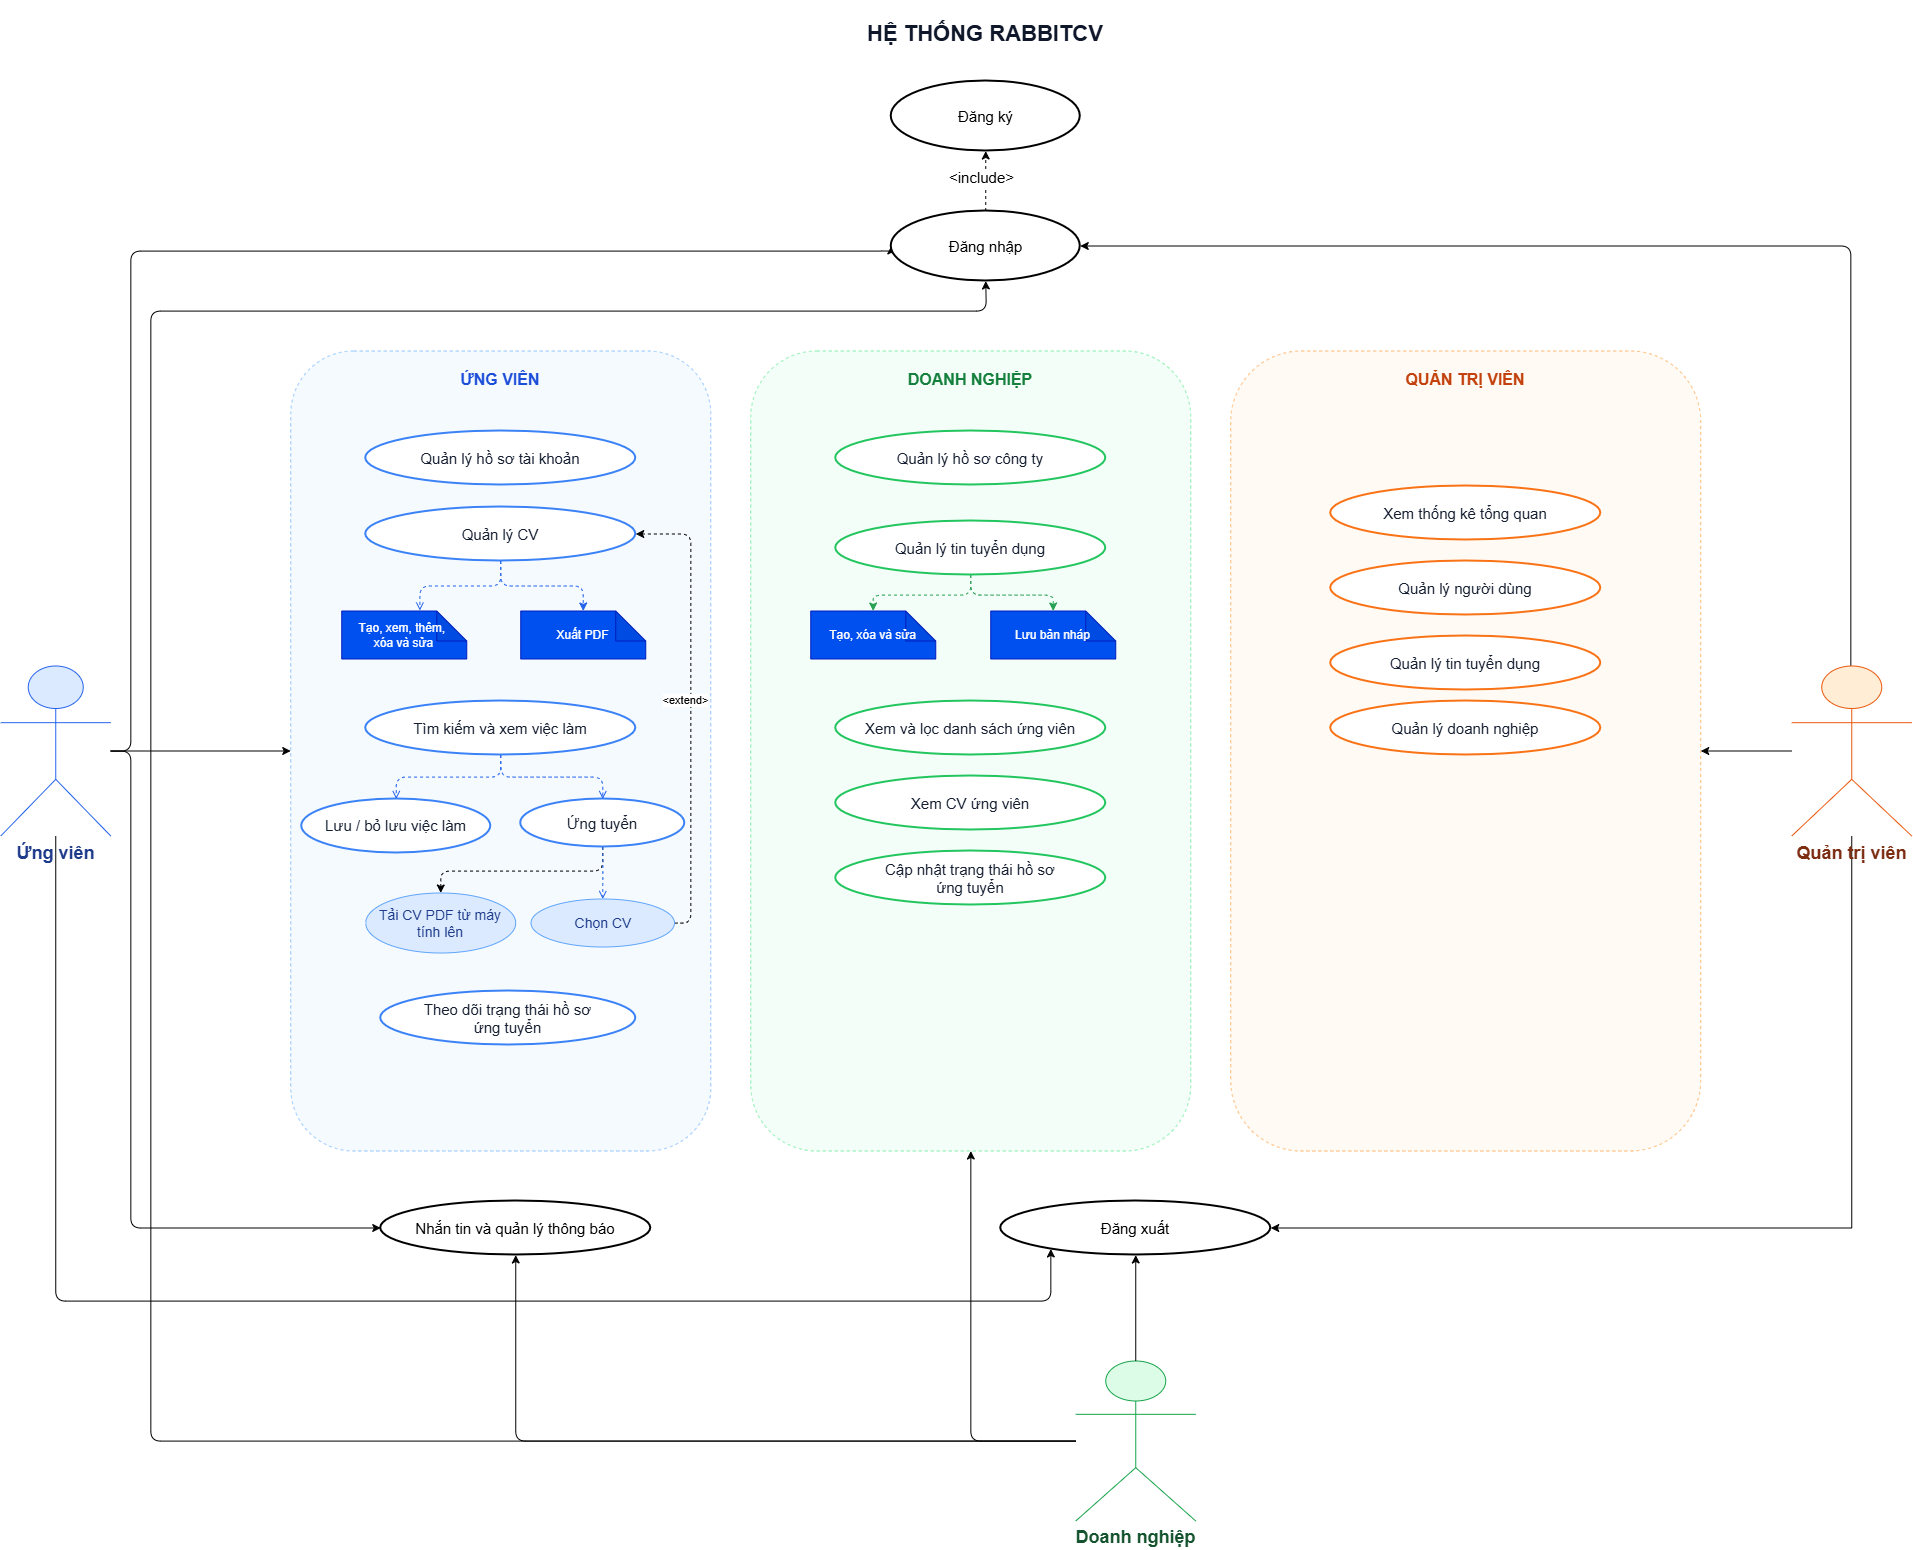
\includegraphics[
        angle=90,
        width=0.98\linewidth,
        height=0.92\textheight,
        keepaspectratio
    ]{img/usecase_overview.png}
    \caption{Lược đồ usecase cho toàn bộ hệ thống}
    \label{fig:usecase-overview}
\end{figure}

\clearpage

\section{Đặc tả usecase}

\subsection{Quản lý tài khoản, CV và tính năng AI}

\begin{figure}[H]
    \centering
    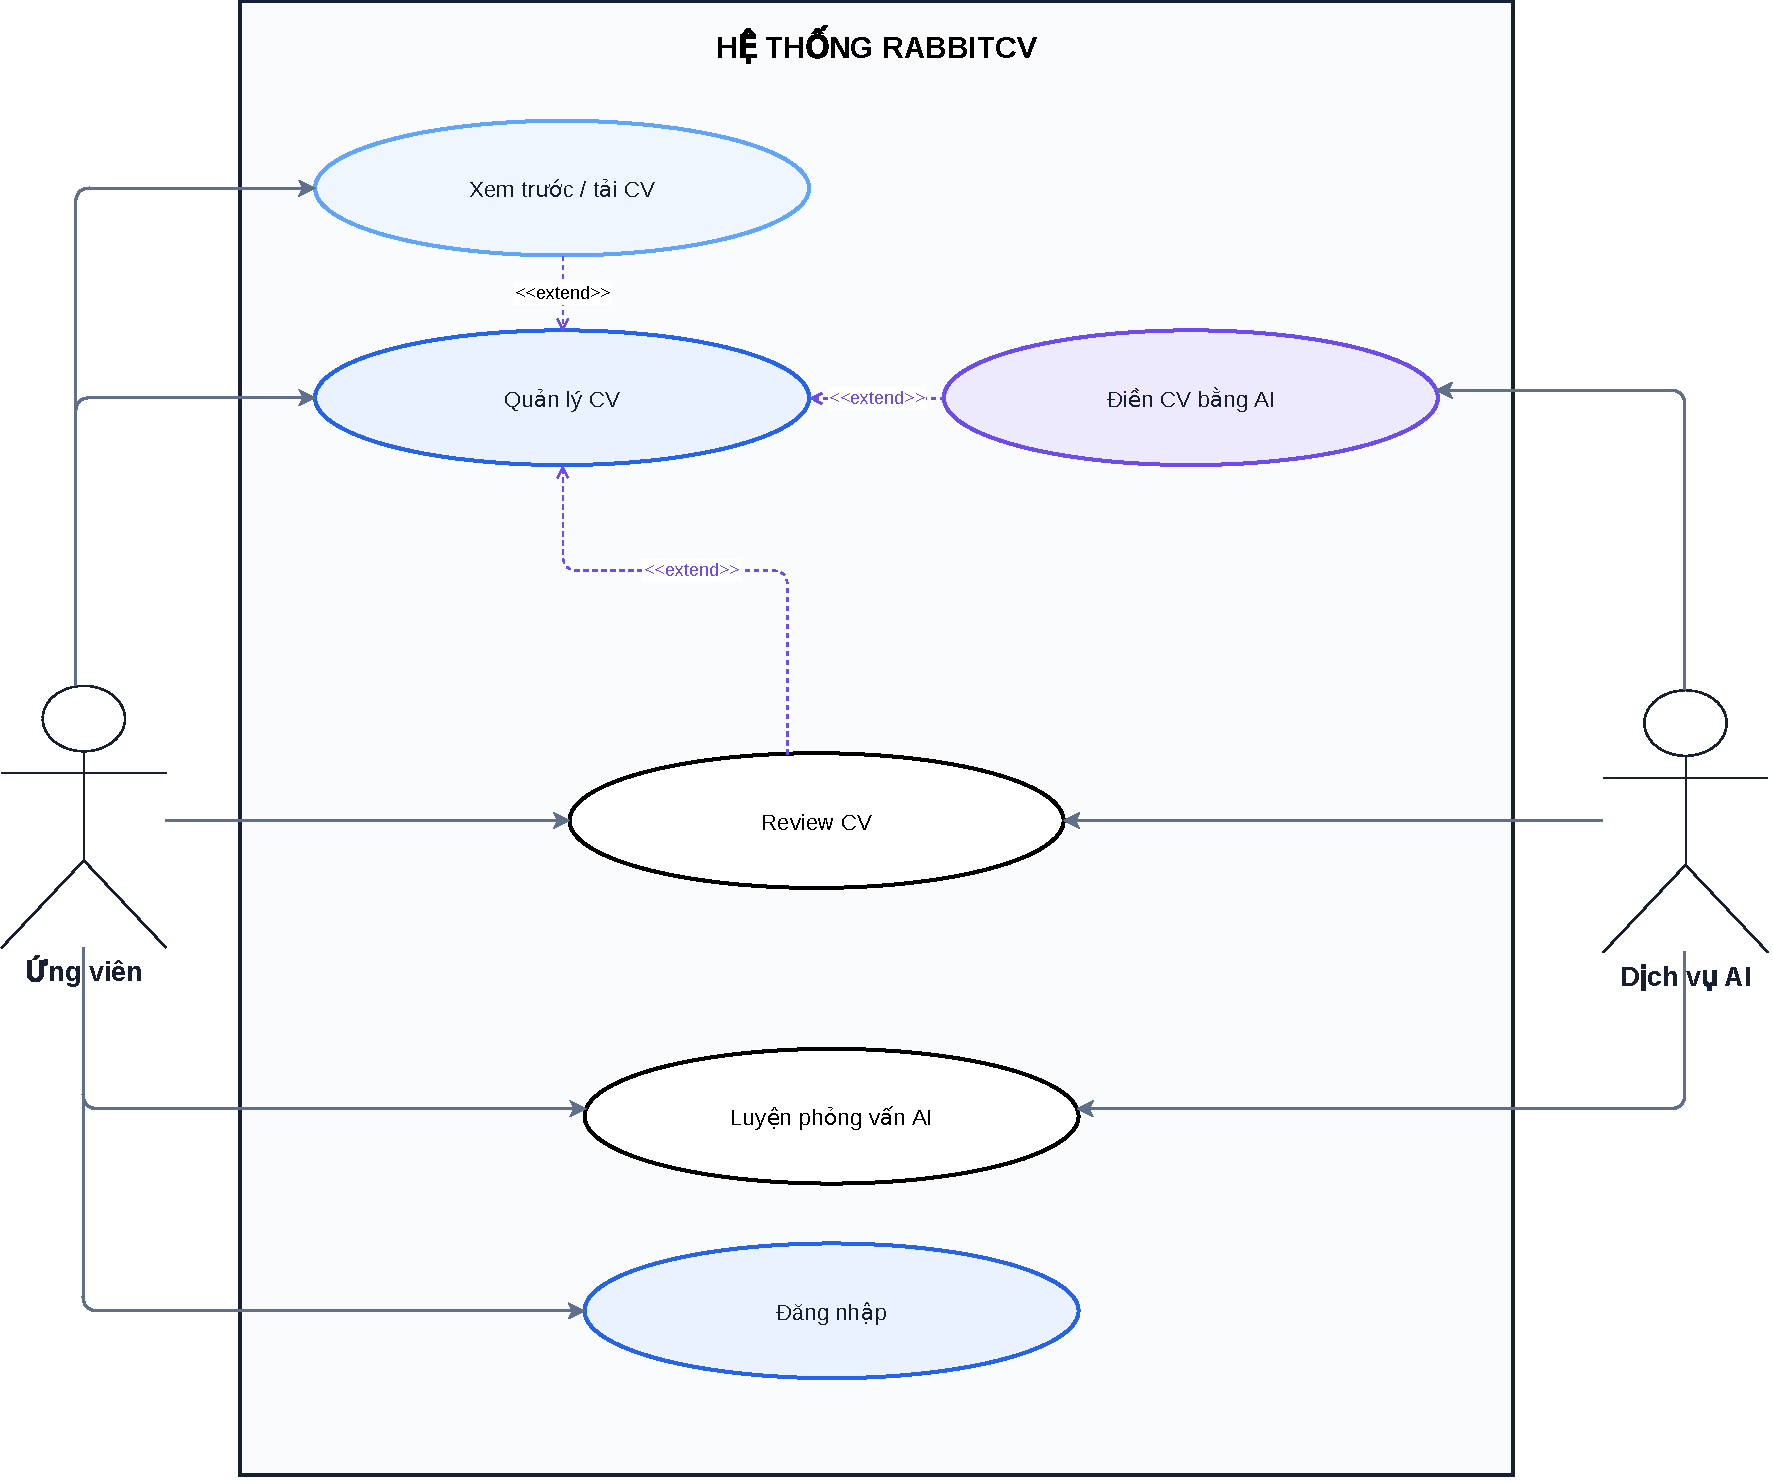
\includegraphics[
        width=0.85\linewidth,
        height=0.50\textheight,
        keepaspectratio
    ]{img/CV-usecase.pdf}
    \caption{Lược đồ usecase quản lý CV}
    \label{fig:uc-cv}
\end{figure}

\begin{table}[H]
    \centering
    \small
    \renewcommand{\arraystretch}{1.0}
    \begin{tabularx}{\textwidth}{|
        >{\bfseries\raggedright\arraybackslash}p{3.2cm}|Y|}
        \hline

        Usecase ID& CV-1.1 \\ \hline

        Tên use case & Đăng nhập \\ \hline

        Đối tượng & Người dùng \\ \hline

        Mô tả & Cho phép người dùng đăng nhập vào hệ thống \\ \hline

        Tiền điều kiện &
        \parbox[t]{\hsize}{
            1.\ Người dùng chưa đăng nhập vào hệ thống.\par
            2.\ Người dùng đã đăng ký tài khoản và có thông tin trong hệ thống.\par
        } \\
        \hline

        Hậu điều kiện & Người dùng đăng nhập thành công \\ \hline

        Luồng thực hiện chính&
        \parbox[t]{\hsize}{
            1.\ Người dùng nhấn vào nút Đăng nhập\par
            2.\ Hệ thống chuyển sang trang đăng nhập\par
            3.\ Người dùng nhập thông tin tài khoản và mật khẩu\par
            4.\ Hệ thống xác thực thông tin tài khoản\par
            5.\ Người dùng đăng nhập thành công}\\
        \hline

        Luồng thực hiện phụ& Không có \\
        \hline

        Lỗi &
        \parbox[t]{\hsize}{
            E1. Tên đăng nhập hoặc mật khẩu không chính xác\\
            E2. Tài khoản đã bị khóa hoặc ngừng hoạt động bởi quản trị viên\\
            E3. Mất kết nối mạng hoặc máy chủ không phản hồi\\
            E4. Hệ thống đang bảo trì định kỳ
        }\\
        \hline

    \end{tabularx}

    \caption{Use case CV-1.1: Đăng nhập}
    \label{tab:usecase-cv11}
\end{table}


\begin{table}[H]
    \centering
    \small
    \renewcommand{\arraystretch}{1.0}
    \begin{tabularx}{\textwidth}{|
        >{\bfseries\raggedright\arraybackslash}p{3.2cm}|Y|}
        \hline

        Usecase ID& CV-1.2 \\ \hline

        Tên use case & Đăng ký \\ \hline

        Đối tượng & Người dùng \\ \hline

        Mô tả & Cho phép người dùng đăng ký tài khoản vào hệ thống \\ \hline

        Tiền điều kiện &
        \parbox[t]{\hsize}{
            Người dùng chưa đăng nhập vào hệ thống.\par
        } \\
        \hline

        Hậu điều kiện & Tài khoản được tạo thành công; tài khoản doanh nghiệp tự đăng ký có trạng thái chờ phê duyệt \\ \hline

        Luồng thực hiện chính&
        \parbox[t]{\hsize}{
            1.\ Người dùng nhấn vào nút Đăng ký\par
            2.\ Hệ thống chuyển sang trang đăng ký\par
            3.\ Người dùng nhập tên đăng nhập, email, mật khẩu, xác nhận mật khẩu, chọn vai trò và đồng ý điều khoản; nếu chọn Doanh nghiệp thì nhập thêm tên doanh nghiệp\par
            4.\ Hệ thống kiểm tra dữ liệu, tên đăng nhập và email chưa được sử dụng\par
            5.\ Hệ thống tạo tài khoản và chuyển tới giao diện tương ứng; tài khoản doanh nghiệp được thông báo cần quản trị viên phê duyệt trước khi đăng tin}\\
        \hline

        Luồng thực hiện phụ& Không có \\
        \hline

        Lỗi &
        \parbox[t]{\hsize}{
            E1. Thông tin đăng ký không hợp lệ (email sai định dạng, xác nhận mật khẩu không khớp)\\
            E2. Tên đăng nhập hoặc email đã tồn tại trong hệ thống\\
            E3. Mất kết nối mạng hoặc lỗi cơ sở dữ liệu khi tạo tài khoản\\
            E4. Hệ thống đang bảo trì
        }\\
        \hline

    \end{tabularx}

    \caption{Use case CV-1.2: Đăng ký}
    \label{tab:usecase-cv12}
\end{table}

\begin{table}[H]
    \centering
    \small
    \renewcommand{\arraystretch}{1.0}
    \begin{tabularx}{\textwidth}{|
        >{\bfseries\raggedright\arraybackslash}p{3.2cm}|Y|}
        \hline

        Usecase ID& CV-1.3 \\ \hline

        Tên use case & Đăng xuất \\ \hline

        Đối tượng & Người dùng \\ \hline

        Mô tả & Cho phép người dùng đăng xuất khỏi hệ thống \\ \hline

        Tiền điều kiện &
        \parbox[t]{\hsize}{
            Người dùng đã đăng nhập vào hệ thống.\par
        } \\
        \hline

        Hậu điều kiện & Người dùng đăng xuất thành công \\ \hline

        Luồng thực hiện chính&
        \parbox[t]{\hsize}{
            1.\ Người dùng nhấn vào nút Đăng xuất\par
            2.\ Hệ thống hủy phiên đăng nhập và chuyển hướng về trang chủ}\\
        \hline

        Luồng thực hiện phụ& Không có \\
        \hline

        Lỗi &
        \parbox[t]{\hsize}{
            E1. Phiên đăng nhập đã hết hạn hoặc không còn hiệu lực trên máy chủ\\
            E2. Mất kết nối mạng làm gián đoạn yêu cầu hủy phiên
        }\\
        \hline

    \end{tabularx}

    \caption{Use case CV-1.3: Đăng xuất}
    \label{tab:usecase-cv13}
\end{table}


\begin{table}[H]
    \centering
    \small
    \renewcommand{\arraystretch}{1.0}
    \begin{tabularx}{\textwidth}{|
        >{\bfseries\raggedright\arraybackslash}p{3.2cm}|Y|}
        \hline

        Usecase ID& CV-1.4 \\ \hline

        Tên use case & Quản lý thông tin tài khoản \\ \hline

        Đối tượng & Người dùng \\ \hline

        Mô tả & Cho phép người dùng quản lý thông tin tài khoản \\ \hline

        Tiền điều kiện &
        \parbox[t]{\hsize}{
            Người dùng đã đăng nhập vào hệ thống.\par
        } \\
        \hline

        Hậu điều kiện & Người dùng cập nhật thông tin tài khoản thành công \\ \hline

        Luồng thực hiện chính&
        \parbox[t]{\hsize}{
            1.\ Người dùng nhấn vào icon người dùng\par
            2.\ Dropdown hiển thị các tùy chọn: Hồ sơ của tôi, Việc làm của tôi, Cài đặt và Đăng xuất\par
            3.\ Người dùng nhấn vào "Hồ sơ của tôi"\par
            4.\ Hệ thống chuyển sang trang hồ sơ cá nhân\par
            5.\ Người dùng cập nhật thông tin tài khoản\par
            6.\ Hệ thống lưu thông tin tài khoản và hiển thị thông báo thành công}\\
        \hline

        Luồng thực hiện phụ& Không có \\
        \hline

        Lỗi &
        \parbox[t]{\hsize}{
            E1. Dữ liệu cập nhật không hợp lệ (định dạng email, số điện thoại, ngày sinh sai chuẩn)\\
            E2. Địa chỉ email mới đã được sử dụng bởi một tài khoản khác trong hệ thống\\
            E3. Phiên đăng nhập hết hạn hoặc mất kết nối máy chủ khi lưu thông tin
        }\\
        \hline

    \end{tabularx}

    \caption{Use case CV-1.4: Quản lý thông tin tài khoản}
    \label{tab:usecase-cv14}
\end{table}



\begin{table}[H]
    \centering
    \small
    \renewcommand{\arraystretch}{0.95}
    \begin{tabularx}{\textwidth}{|
        >{\bfseries\raggedright\arraybackslash}p{2.6cm}|Y|}
        \hline

        Usecase ID & CV-1.5 \\ \hline

        Tên use case & Quản lý CV \\ \hline

        Đối tượng & Ứng viên \\ \hline

        Mô tả & Cho phép ứng viên quản lý, tạo mới, chỉnh sửa, đổi tên hoặc xóa CV cá nhân \\ \hline

        Tiền điều kiện &
        \parbox[t]{\hsize}{
            1. Ứng viên đã đăng nhập vào hệ thống.\\
            2. Ứng viên đang ở trang quản lý/dashboard.
        } \\
        \hline

        Hậu điều kiện & CV được tạo mới, cập nhật, đổi tên hoặc xóa theo thao tác của ứng viên \\ \hline

        Luồng thực hiện chính &
        \parbox[t]{\hsize}{
            1.\ Ứng viên nhấn vào tab ``Tạo CV'' và lựa chọn mẫu CV mong muốn\\
            2.\ Hệ thống hiển thị trang điền thông tin theo mẫu CV đã chọn\\
            3.\ Ứng viên nhập đầy đủ thông tin vào các mục theo yêu cầu\\
            4.\ Ứng viên nhấn nút ``Lưu'', hệ thống kiểm tra dữ liệu và thông báo lưu thành công
        }\\
        \hline

        Luồng thực hiện phụ &
        \parbox[t]{\hsize}{
            1.\ Từ danh sách CV, ứng viên chọn CV của mình để chỉnh sửa, đổi tên hoặc xóa\\
            2.\ Hệ thống kiểm tra quyền sở hữu và thực hiện thao tác; cập nhật được ghi nhận khi nhấn ``Lưu''\\
            3.\ Bản CV đã nộp trong các hồ sơ ứng tuyển trước đó vẫn được bảo lưu nguyên vẹn
        }\\
        \hline

        Lỗi &
        \parbox[t]{\hsize}{
            E1. CV cần truy cập không tồn tại hoặc không thuộc quyền sở hữu của ứng viên\\
            E2. Mất kết nối máy chủ trong quá trình lưu dữ liệu CV vào cơ sở dữ liệu\\
            E3. Dữ liệu CV không hợp lệ (tiêu đề trống hoặc chưa đúng định dạng)\\
            E4. Hệ thống đang bảo trì định kỳ
        }\\
        \hline

    \end{tabularx}
    \caption{Use case CV-1.5: Quản lý CV}
    \label{tab:usecase-cv15}
\end{table}

\begin{table}[H]
    \centering
    \small
    \renewcommand{\arraystretch}{0.95}
    \begin{tabularx}{\textwidth}{|
        >{\bfseries\raggedright\arraybackslash}p{2.6cm}|Y|}
        \hline

        Usecase ID & CV-1.6 \\ \hline

        Tên use case & Tải CV \\ \hline

        Đối tượng & Ứng viên \\ \hline

        Mô tả & Cho phép ứng viên xuất CV có cấu trúc thành tệp PDF qua hộp thoại in của trình duyệt \\ \hline

        Tiền điều kiện &
        \parbox[t]{\hsize}{
            1. Ứng viên đã đăng nhập vào hệ thống và đang ở trang danh sách CV.\\
            2. Ứng viên đã tạo ít nhất 1 bản CV trong hệ thống.
        } \\
        \hline

        Hậu điều kiện & Hộp thoại in được mở; ứng viên có thể lưu PDF hoặc hủy mà không đổi dữ liệu CV \\ \hline

        Luồng thực hiện chính &
        \parbox[t]{\hsize}{
            \textbf{Tải PDF từ danh sách CV:}\\
            1.\ Ứng viên lựa chọn bản CV muốn tải và nhấn nút ``Tải PDF''\\
            2.\ Hệ thống dựng nội dung CV và tự động mở hộp thoại in của trình duyệt\\
            3.\ Ứng viên chọn lưu thành PDF, chọn vị trí lưu hoặc hủy thao tác
        }\\
        \hline

        Luồng thực hiện phụ & 
        \parbox[t]{\hsize}{
            \textbf{Tải PDF từ màn hình chỉnh sửa CV:}\\
            1.\ Ứng viên bấm nút ``Chỉnh sửa'' tại hàng CV tương ứng trong danh sách\\
            2.\ Hệ thống chuyển sang trang soạn thảo với nội dung CV đã lưu\\
            3.\ Ứng viên chỉnh sửa nội dung mong muốn và bấm nút ``Tải PDF''\\
            4.\ Hệ thống mở hộp thoại in cho nội dung đang hiển thị (không tự lưu vào cơ sở dữ liệu)
        }\\
        \hline

        Lỗi &
        \parbox[t]{\hsize}{
            E1. Không tải được dữ liệu CV hoặc CV không thuộc quyền sở hữu của ứng viên\\
            E2. Trình duyệt không mở được hộp thoại in hoặc quá trình dựng bản in thất bại
        }\\
        \hline

    \end{tabularx}
    \caption{Use case CV-1.6: Tải CV}
    \label{tab:usecase-cv16}
\end{table}

\begin{table}[H]
    \centering
    \small
    \renewcommand{\arraystretch}{0.90}
    \begin{tabularx}{\textwidth}{|
        >{\bfseries\raggedright\arraybackslash}p{2.6cm}|Y|}
        \hline

        Usecase ID & CV-1.7 \\ \hline

        Tên use case & Điền CV bằng AI \\ \hline

        Đối tượng & Ứng viên \\ \hline

        Mô tả & Tự động sinh nội dung gợi ý vào các phần còn thiếu của CV bằng AI \\ \hline

        Tiền điều kiện &
        \parbox[t]{\hsize}{
            1. Ứng viên đã đăng nhập vào hệ thống.\\
            2. Ứng viên đang ở trang chỉnh sửa CV.
        } \\
        \hline

        Hậu điều kiện & Gợi ý từ AI được bổ sung vào bản CV; chỉ lưu khi nhấn ``Lưu'' \\ \hline

        Luồng thực hiện chính &
        \parbox[t]{\hsize}{
            1.\ Ứng viên nhấn nút ``Điền CV bằng AI'' trên giao diện chỉnh sửa\\
            2.\ Ứng viên nhập vị trí công việc mong muốn và xác nhận\\
            3.\ Hệ thống gửi ngữ cảnh đến AI và điền gợi ý vào các mục còn thiếu\\
            4.\ Ứng viên rà soát, chỉnh sửa nội dung và nhấn nút ``Lưu''\\
            5.\ Hệ thống xác thực và lưu dữ liệu CV vào cơ sở dữ liệu
        }\\
        \hline

        Luồng thực hiện phụ & Không có \\
        \hline

        Lỗi &
        \parbox[t]{\hsize}{
            E1. Vượt quá hạn mức sử dụng AI hoặc tần suất cho phép\\
            E2. Quá thời gian chờ phản hồi (timeout) từ dịch vụ AI\\
            E3. Phản hồi từ mô hình AI không đúng định dạng JSON Schema\\
            E4. Mất kết nối mạng hoặc gián đoạn dịch vụ AI\\
            E5. Hệ thống đang bảo trì định kỳ
        }\\
        \hline

    \end{tabularx}
    \caption{Use case CV-1.7: Điền CV bằng AI}
    \label{tab:usecase-cv17}
\end{table}

\begin{table}[H]
    \centering
    \small
    \renewcommand{\arraystretch}{0.90}
    \begin{tabularx}{\textwidth}{|
        >{\bfseries\raggedright\arraybackslash}p{2.6cm}|Y|}
        \hline

        Usecase ID & CV-1.8 \\ \hline

        Tên use case & Review CV bằng AI \\ \hline

        Đối tượng & Ứng viên \\ \hline

        Mô tả & Nhận phân tích, chấm điểm và gợi ý cải thiện chất lượng CV từ AI \\ \hline

        Tiền điều kiện &
        \parbox[t]{\hsize}{
            1. Ứng viên đã đăng nhập vào hệ thống.\\
            2. Ứng viên đang ở trang chỉnh sửa CV.
        } \\
        \hline

        Hậu điều kiện & Hiển thị bảng điểm đánh giá CV và các đề xuất cải thiện từ AI \\ \hline

        Luồng thực hiện chính &
        \parbox[t]{\hsize}{
            1.\ Ứng viên nhấn nút ``Review CV'' trên giao diện chỉnh sửa\\
            2.\ Hệ thống phân tích qua AI, hiển thị bảng điểm và các lỗi cần sửa\\
            3.\ Ứng viên kiểm tra đánh giá và chỉnh sửa nội dung CV nếu cần\\
            4.\ Ứng viên nhấn ``Đóng'' hoặc chọn ``Review lại'' để cập nhật
        }\\
        \hline

        Luồng thực hiện phụ & Không có \\
        \hline

        Lỗi &
        \parbox[t]{\hsize}{
            E1. Vượt quá hạn mức yêu cầu AI hoặc tần suất cho phép\\
            E2. Quá thời gian chờ phản hồi từ dịch vụ AI\\
            E3. Phản hồi từ AI không đúng cấu trúc schema đánh giá\\
            E4. Nội dung CV quá ngắn, không đủ dữ liệu để AI phân tích\\
            E5. Mất kết nối tới dịch vụ AI làm gián đoạn xử lý\\
            E6. Hệ thống đang bảo trì định kỳ
        }\\
        \hline

    \end{tabularx}
    \caption{Use case CV-1.8: Review CV bằng AI}
    \label{tab:usecase-cv18}
\end{table}

\begin{table}[H]
    \centering
    \small
    \renewcommand{\arraystretch}{0.95}
    \begin{tabularx}{\textwidth}{|
        >{\bfseries\raggedright\arraybackslash}p{2.6cm}|Y|}
        \hline

        Usecase ID & CV-1.9 \\ \hline

        Tên use case & Phỏng vấn với AI \\ \hline

        Đối tượng & Ứng viên \\ \hline

        Mô tả & Cho phép ứng viên luyện tập phỏng vấn theo các kịch bản tùy chọn và nhận đánh giá từ AI \\ \hline

        Tiền điều kiện &
        \parbox[t]{\hsize}{
            1. Ứng viên đã đăng nhập vào hệ thống.\\
            2. Ứng viên đang ở trang dashboard.
        } \\
        \hline

        Hậu điều kiện & Ứng viên hoàn thành phiên luyện tập phỏng vấn và nhận bảng đánh giá nhận xét chi tiết \\ \hline

        Luồng thực hiện chính &
        \parbox[t]{\hsize}{
            1.\ Ứng viên nhấn vào nút ``Phỏng vấn với AI''\\
            2.\ Hệ thống hiển thị trang lựa chọn cấp độ, hình thức và số lượng câu hỏi\\
            3.\ Ứng viên chọn các yêu cầu mong muốn và nhấn nút ``Bắt đầu phỏng vấn''\\
            4.\ Hệ thống lần lượt đưa ra câu hỏi và yêu cầu ứng viên nhập câu trả lời\\
            5.\ Sau khi trả lời, hệ thống hiển thị đánh giá câu trả lời và gợi ý cải thiện\\
            6.\ Khi kết thúc phiên, hệ thống hiển thị đánh giá tổng quan (kết quả chỉ giữ trong phiên đang mở, không lưu lịch sử vào cơ sở dữ liệu)
        }\\
        \hline

        Luồng thực hiện phụ & Không có \\
        \hline

        Lỗi &
        \parbox[t]{\hsize}{
            E1. Vượt quá hạn mức yêu cầu AI trong ngày hoặc giới hạn tần suất gửi\\
            E2. Quá thời gian chờ phản hồi từ dịch vụ AI\\
            E3. Phản hồi từ mô hình AI không đúng định dạng chuẩn hóa thang điểm và nhận xét\\
            E4. Câu trả lời của ứng viên rỗng hoặc chứa nội dung không hợp lệ\\
            E5. Mất kết nối tới dịch vụ AI làm gián đoạn quá trình xử lý\\
            E6. Hệ thống đang bảo trì định kỳ
        }\\
        \hline

    \end{tabularx}
    \caption{Use case CV-1.9: Phỏng vấn với AI}
    \label{tab:usecase-cv19}
\end{table}

\clearpage
\subsection{Tìm việc và ứng tuyển việc làm}

\begin{figure}[H]
    \centering
    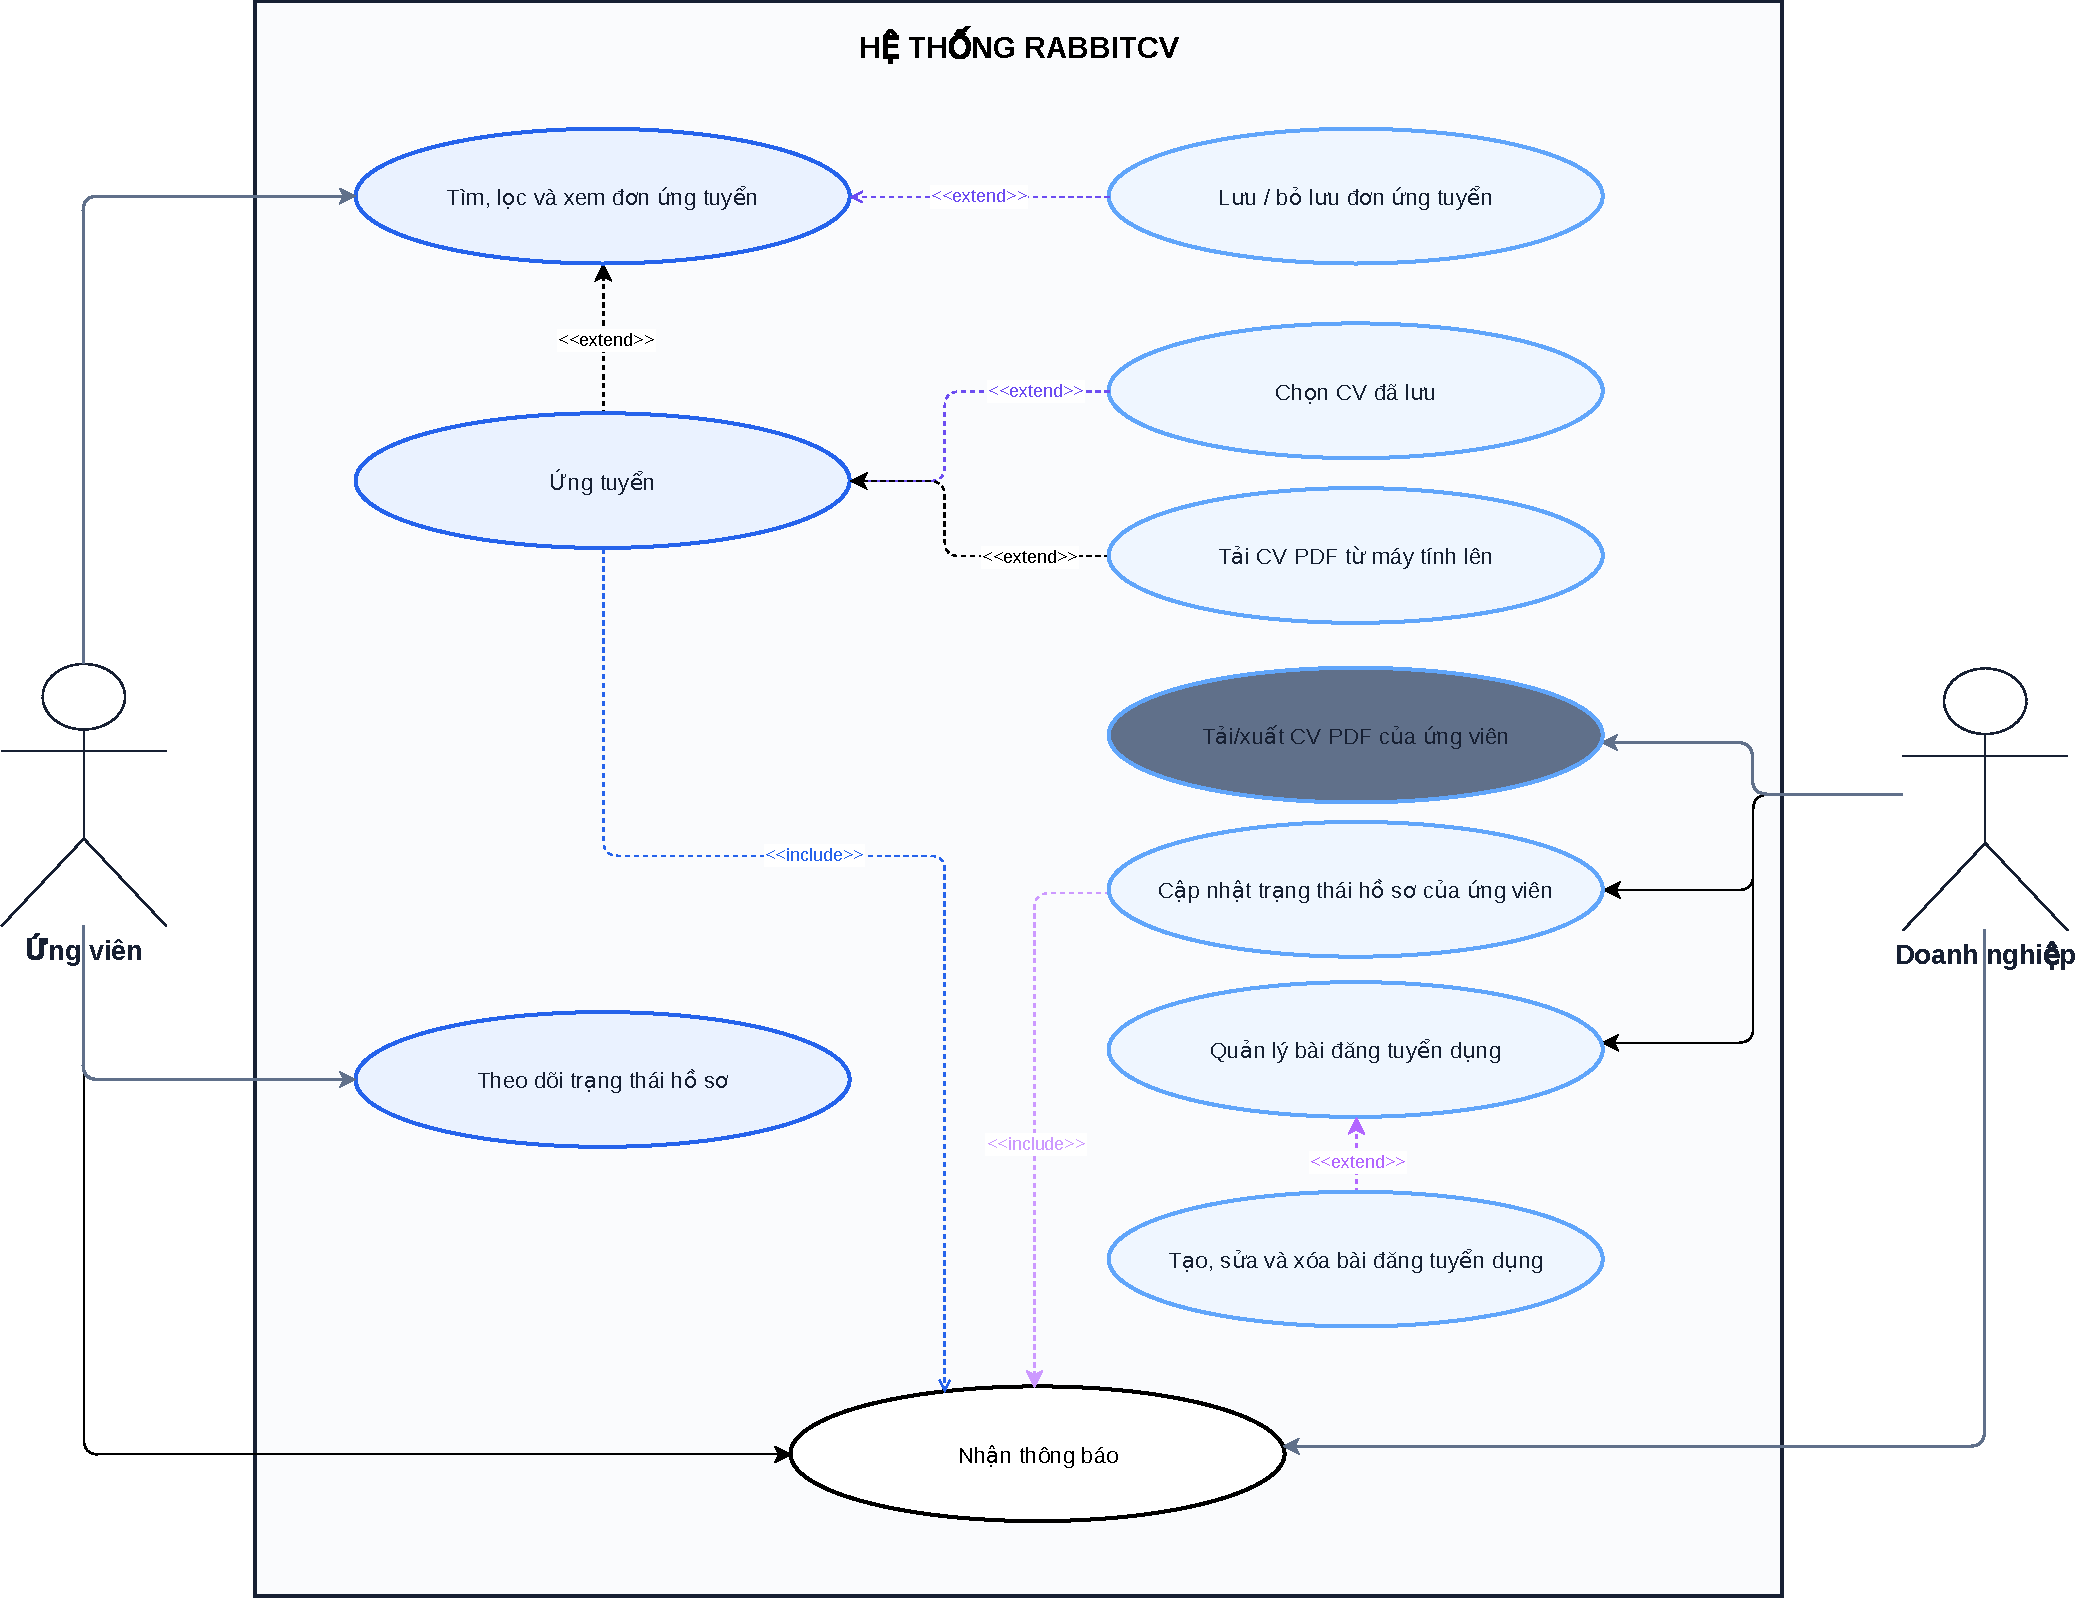
\includegraphics[
        width=0.85\linewidth,
        height=0.50\textheight,
        keepaspectratio
    ]{img/usecase-Jobs.pdf}
    \caption{Lược đồ usecase tìm việc và ứng tuyển việc làm}
    \label{fig:uc-jobs}
\end{figure}


\begin{table}[H]
    \centering
    \small
    \renewcommand{\arraystretch}{1.0}
    \begin{tabularx}{\textwidth}{|
        >{\bfseries\raggedright\arraybackslash}p{3.2cm}|Y|}
        \hline

        Usecase ID& CV-2.1 \\ \hline

        Tên use case & Tìm kiếm việc làm\\ \hline

        Đối tượng & Khách, Ứng viên \\ \hline

        Mô tả & Cho phép người dùng tra cứu và lọc các tin tuyển dụng công khai mà không bắt buộc đăng nhập\\ \hline

        Tiền điều kiện &
        \parbox[t]{\hsize}{
            Người dùng truy cập trang "Tìm kiếm việc làm"; không yêu cầu đã đăng nhập.\par
        } \\
        \hline

        Hậu điều kiện & Danh sách tin phù hợp được hiển thị, hoặc hệ thống hiển thị trạng thái không có kết quả \\ \hline

        Luồng thực hiện chính&
        \parbox[t]{\hsize}{
            1.\ Người dùng nhập từ khóa hoặc chọn tiêu chí lọc và nhấn nút tìm kiếm\\
            2.\ Hệ thống hiển thị các tin công khai, còn nhận hồ sơ và phù hợp với điều kiện tìm kiếm\\
            3.\ Người dùng chọn một tin để xem chi tiết công việc và thông tin doanh nghiệp
        }\\
        \hline

        Luồng thực hiện phụ&
        \parbox[t]{\hsize}{
            1.\ Nếu không nhập từ khóa hoặc chọn bộ lọc, hệ thống hiển thị danh sách tin theo điều kiện mặc định\\
            2.\ Nếu không có tin phù hợp, hệ thống hiển thị danh sách rỗng và cho phép thay đổi điều kiện tìm kiếm\\
            3.\ Khách muốn lưu tin hoặc ứng tuyển phải đăng nhập bằng tài khoản ứng viên
        }\\
        \hline
        

        Lỗi
        & E1. Mất kết nối hoặc máy chủ không tải được danh sách tin tuyển dụng\\
        & E2. Tin được chọn không còn công khai hoặc không còn nhận hồ sơ khi mở trang chi tiết\\
        \hline

    \end{tabularx}

    \caption{Use case CV-2.1: Tìm kiếm việc làm}
    \label{tab:usecase-cv21}
\end{table}


\begin{table}[H]
    \centering
    \small
    \renewcommand{\arraystretch}{1.0}
    \begin{tabularx}{\textwidth}{|
        >{\bfseries\raggedright\arraybackslash}p{3.2cm}|Y|}
        \hline

        Usecase ID& CV-2.2 \\ \hline

        Tên use case & Ứng tuyển việc làm\\ \hline

        Đối tượng & Ứng viên \\ \hline

        Mô tả & Cho phép ứng viên ứng tuyển việc làm\\ \hline

        Tiền điều kiện &
        \parbox[t]{\hsize}{
            1. Ứng viên đã đăng nhập vào hệ thống.\par
            2. Tin tuyển dụng đang công khai, còn nhận hồ sơ và ứng viên chưa nộp hồ sơ vào tin này.\par
        } \\
        \hline

        Hậu điều kiện & Hồ sơ được tạo với trạng thái \texttt{Pending}, kèm bản chụp CV và tin tuyển dụng; ứng viên và doanh nghiệp nhận thông báo tương ứng \\ \hline

        Luồng thực hiện chính&
        \parbox[t]{\hsize}{
            1.\ Ứng viên lựa chọn CV đã lưu thuộc sở hữu của mình để ứng tuyển\\
            2.\ Ứng viên bấm vào nút "Ứng tuyển bằng CV đã tạo" \\
            3.\ Hệ thống kiểm tra tin, quyền sở hữu CV và việc nộp trùng; tạo hồ sơ cùng bản chụp CV, thông tin việc làm và hiển thị thông báo ứng tuyển thành công
        }\\
        \hline

        Luồng thực hiện phụ&
        \parbox[t]{\hsize}{
            1.\ Ứng viên bấm vào nút "Tải CV PDF từ máy"\\
            2.\ Ứng viên chọn tệp CV PDF từ thiết bị với dung lượng không vượt quá 5~MB\\
            3.\ Hệ thống hiển thị thông tin tệp đã chọn\\
            4.\ Ứng viên bấm vào nút "Ứng tuyển bằng CV vừa tải lên"\\
            5.\ Hệ thống kiểm tra tệp, tin tuyển dụng và việc nộp trùng; lưu hồ sơ kèm bản CV PDF đã nộp và hiển thị thông báo ứng tuyển thành công
        }\\
        \hline
        

        Lỗi
        & E1. Hệ thống đang bảo trì\\
        & E2. Ứng viên chưa chọn CV, CV không tồn tại hoặc không thuộc ứng viên\\
        & E3. CV tải lên bị lỗi, sai định dạng hoặc vượt quá giới hạn 5MB\\
        & E4. Ứng viên đã ứng tuyển vào tin tuyển dụng này rồi\\
        & E5. Tin tuyển dụng đã hết hạn nộp hồ sơ, đã đóng hoặc bị xóa khỏi hệ thống\\
        \hline

    \end{tabularx}

    \caption{Use case CV-2.2: Ứng tuyển việc làm}
    \label{tab:usecase-cv22}
\end{table}

\begin{table}[H]
    \centering
    \small
    \renewcommand{\arraystretch}{1.0}
    \begin{tabularx}{\textwidth}{|
        >{\bfseries\raggedright\arraybackslash}p{3.2cm}|Y|}
        \hline

        Usecase ID& CV-2.3 \\ \hline

        Tên use case & Theo dõi trạng thái ứng tuyển\\ \hline

        Đối tượng & Ứng viên \\ \hline

        Mô tả & Cho phép ứng viên theo dõi trạng thái ứng tuyển công việc\\ \hline

        Tiền điều kiện &
        \parbox[t]{\hsize}{
            1. Ứng viên đã đăng nhập vào hệ thống.\par
            2. Ứng viên đang ở trang dashboard\par
        } \\
        \hline

        Hậu điều kiện & Ứng viên theo dõi trạng thái ứng tuyển thành công \\ \hline

        Luồng thực hiện chính&
        \parbox[t]{\hsize}{
            1.\ Ứng viên bấm vào nút "Công việc của tôi"\\
            2.\ Hệ thống hiển thị danh sách công việc mà ứng viên đã ứng tuyển\\
            3.\ Ứng viên xem trạng thái xử lý của từng hồ sơ và thông tin việc làm đã được lưu tại thời điểm nộp
        }\\
        \hline

        Luồng thực hiện phụ&
        \parbox[t]{\hsize}{
            1.\ Nếu chưa có hồ sơ, hệ thống hiển thị danh sách rỗng và gợi ý tìm việc\\
            2.\ Nếu tin gốc đã bị xóa mềm hoặc thay đổi, hồ sơ vẫn được hiển thị bằng thông tin đã lưu; đường dẫn đến tin gốc có thể không còn khả dụng
        }\\
        \hline
        

        Lỗi &
        \parbox[t]{\hsize}{
            E1. Phiên đăng nhập hết hạn hoặc không còn hợp lệ\\
            E2. Mất kết nối máy chủ khi tải danh sách hồ sơ ứng tuyển
        }\\
        \hline

    \end{tabularx}

    \caption{Use case CV-2.3: Theo dõi trạng thái ứng tuyển công việc}
    \label{tab:usecase-cv23}
\end{table}
\clearpage
\subsection{Giao tiếp và thông báo}\label{subsec:use-case-cv-3}

\begin{figure}[H]
    \centering
    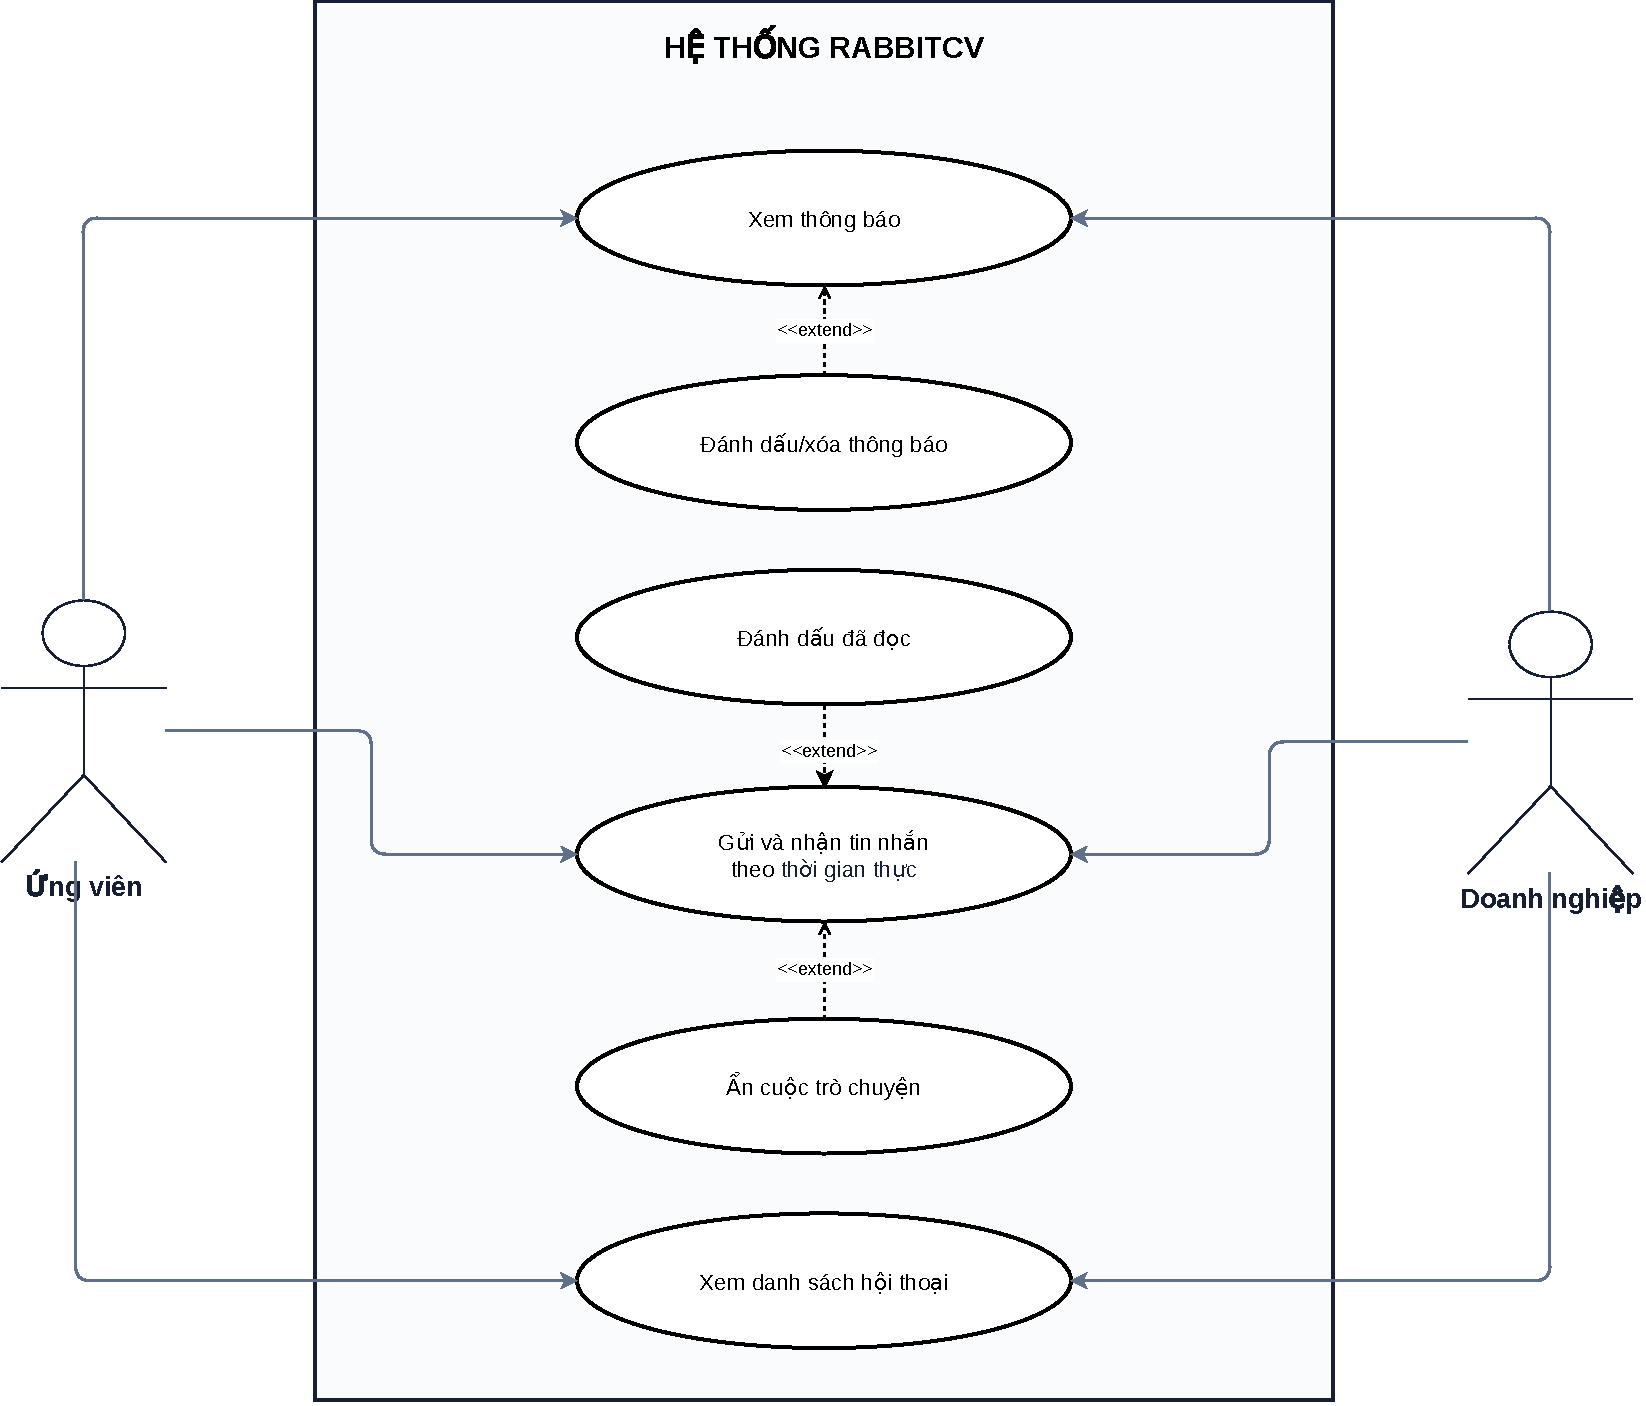
\includegraphics[
        width=0.62\linewidth,
        height=0.30\textheight,
        keepaspectratio
    ]{img/ChatAndNotification-usecase.pdf}
    \caption{Lược đồ usecase giao tiếp và thông báo}
    \label{fig:uc-chat-notification}
\end{figure}

\begin{table}[H]
    \centering
    \small
    \renewcommand{\arraystretch}{1.0}
    \begin{tabularx}{\textwidth}{|
        >{\bfseries\raggedright\arraybackslash}p{3.2cm}|Y|}
        \hline

        Usecase ID & CV-3.1 \\ \hline

        Tên use case & Nhắn tin trao đổi trực tiếp \\ \hline

        Đối tượng & Ứng viên, Doanh nghiệp \\ \hline

        Mô tả & Cho phép ứng viên và doanh nghiệp trò chuyện, trao đổi thông tin công việc hoặc hẹn lịch phỏng vấn theo thời gian thực \\ \hline

        Tiền điều kiện &
        \parbox[t]{\hsize}{
            1. Người dùng đã đăng nhập vào hệ thống.\par
            2. Cuộc hội thoại đã được tạo (từ hồ sơ ứng tuyển hoặc danh sách tin nhắn)
        } \\
        \hline

        Hậu điều kiện & Tin nhắn được lưu và hiển thị cho người gửi; người nhận đang kết nối nhận sự kiện mới, người chưa kết nối có thể tải lịch sử khi mở hội thoại \\ \hline

        Luồng thực hiện chính &
        \parbox[t]{\hsize}{
            1.\ Người dùng nhấn biểu tượng tin nhắn hoặc chọn nút "Nhắn tin" từ hồ sơ ứng tuyển\\
            2.\ Hệ thống tải danh sách hội thoại và hiển thị lịch sử tin nhắn của phòng chat đã chọn\\
            3.\ Người dùng nhập nội dung văn bản vào ô soạn thảo và nhấn nút "Gửi"\\
            4.\ Hệ thống kiểm tra quyền hợp lệ, lưu tin nhắn và phát sự kiện mới qua Socket.IO\\
            5.\ Người nhận đang kết nối nhận sự kiện và giao diện hội thoại được cập nhật; nếu chưa kết nối, tin nhắn vẫn được giữ trong lịch sử
        }\\
        \hline

        Luồng thực hiện phụ &
        \parbox[t]{\hsize}{
            1.\ Người dùng chọn ẩn một cuộc hội thoại trong danh sách\\
            2.\ Hệ thống cập nhật trạng thái ẩn cuộc trò chuyện của người dùng hiện tại
        }\\
        \hline

        Lỗi &
        \parbox[t]{\hsize}{
            E1. Mất kết nối Socket.IO thời gian thực\\
            E2. Người dùng không có quyền truy cập vào phòng chat\\
            E3. Nội dung tin nhắn để trống hoặc vượt quá độ dài ký tự tối đa cho phép\\
            E4. Hệ thống đang bảo trì hoặc máy chủ gặp sự cố
        }\\
        \hline

    \end{tabularx}

    \caption{Use case CV-3.1: Nhắn tin trao đổi trực tiếp}
    \label{tab:usecase-cv31}
\end{table}

\begin{table}[H]
    \centering
    \small
    \renewcommand{\arraystretch}{1.0}
    \begin{tabularx}{\textwidth}{|
        >{\bfseries\raggedright\arraybackslash}p{3.2cm}|Y|}
        \hline

        Usecase ID & CV-3.2 \\ \hline

        Tên use case & Xem và quản lý thông báo \\ \hline

        Đối tượng & Ứng viên, Doanh nghiệp \\ \hline

        Mô tả & Cho phép người dùng nhận, theo dõi và quản lý các thông báo tự động từ hệ thống (kết quả nộp đơn, ứng viên mới, cập nhật tuyển dụng) \\ \hline

        Tiền điều kiện & Người dùng đã đăng nhập vào hệ thống \\ \hline

        Hậu điều kiện & Danh sách thông báo được hiển thị; thông báo được chọn hoặc toàn bộ thông báo được đánh dấu đã đọc theo thao tác của người dùng \\ \hline

        Luồng thực hiện chính &
        \parbox[t]{\hsize}{
            1.\ Người dùng nhấn vào biểu tượng chuông thông báo trên thanh điều hướng\\
            2.\ Hệ thống hiển thị danh sách thông báo mới nhất kèm số lượng chưa đọc, nhận sự kiện mới qua Socket.IO và truy vấn định kỳ để đồng bộ dữ liệu\\
            3.\ Người dùng nhấn chọn một thông báo cụ thể\\
            4.\ Hệ thống cập nhật thông báo sang "Đã đọc" và điều hướng tới trang tương ứng
        }\\
        \hline

        Luồng thực hiện phụ &
        \parbox[t]{\hsize}{
            1.\ Người dùng nhấn nút "Đánh dấu tất cả đã đọc"\\
            2.\ Hệ thống cập nhật toàn bộ danh sách thông báo sang trạng thái đã đọc
        }\\
        \hline

        Lỗi &
        \parbox[t]{\hsize}{
            E1. Hệ thống đang bảo trì\\
            E2. Mất kết nối mạng hoặc lỗi đồng bộ API định kỳ\\
            E3. Nội dung liên kết trong thông báo không còn khả dụng
        }\\
        \hline

    \end{tabularx}

    \caption{Use case CV-3.2: Xem và quản lý thông báo}
    \label{tab:usecase-cv32}
\end{table}

\subsection{Quản lý tuyển dụng và doanh nghiệp}


\begin{figure}[H]
    \centering
    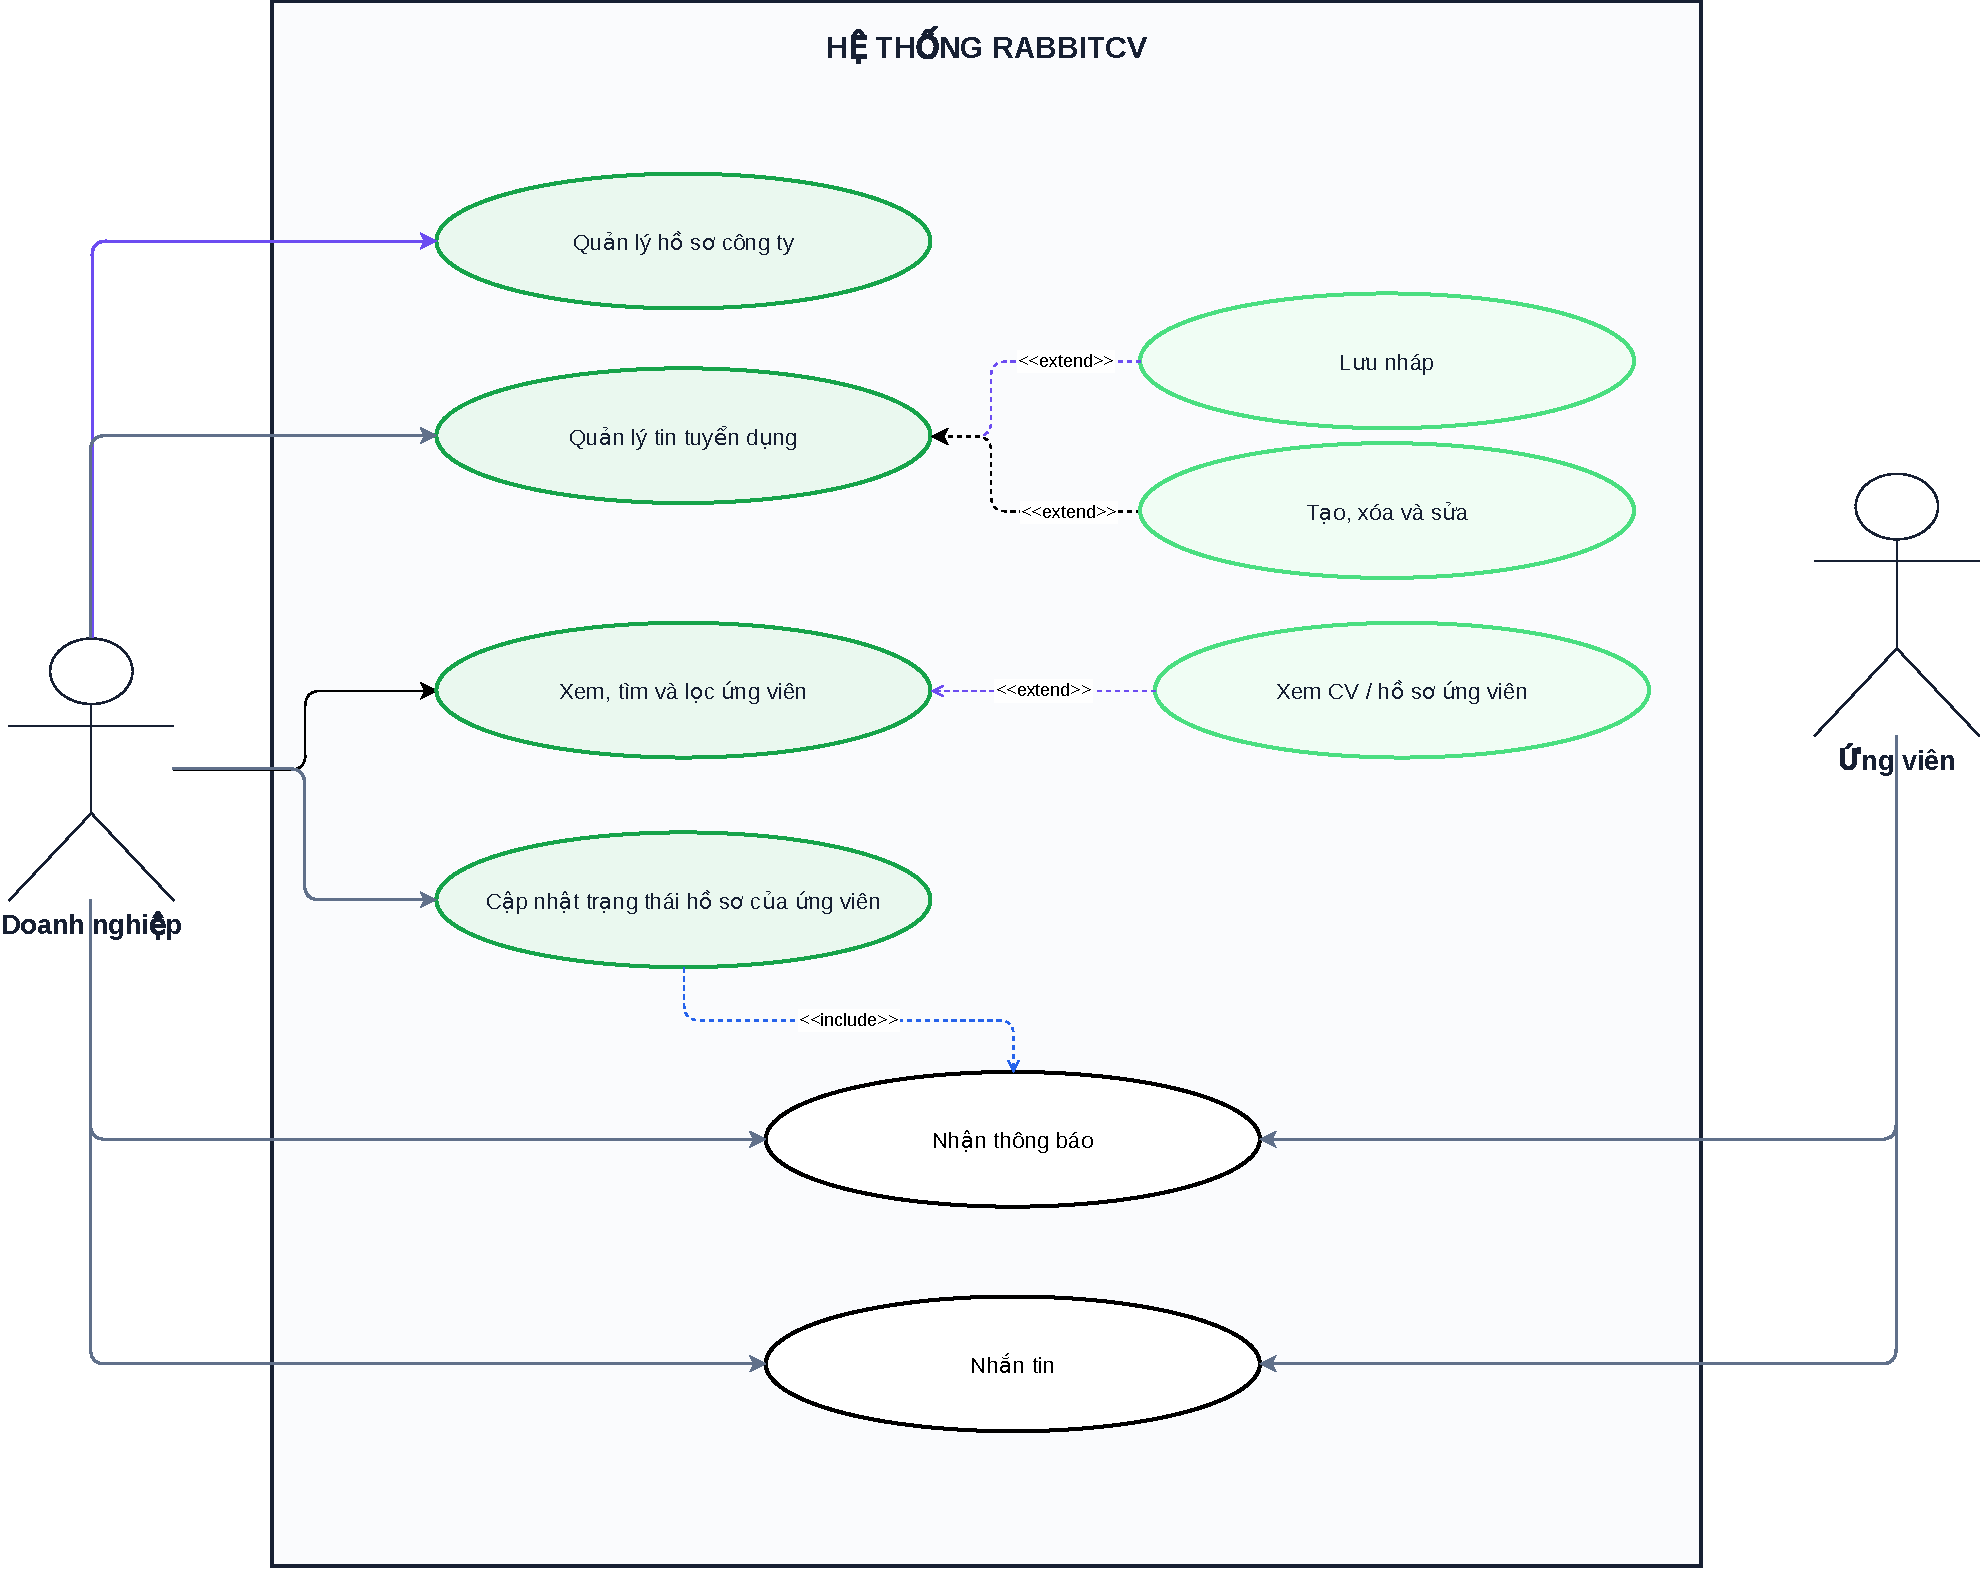
\includegraphics[
        width=0.85\linewidth,
        height=0.50\textheight,
        keepaspectratio
    ]{img/CompanyProfileManagement-usecase.pdf}
    \caption{Lược đồ usecase quản lý thông tin doanh nghiệp}
    \label{fig:uc-company-profile-management}
\end{figure}



\begin{table}[H]
    \centering
    \small
    \renewcommand{\arraystretch}{1.0}
    \begin{tabularx}{\textwidth}{|
        >{\bfseries\raggedright\arraybackslash}p{3.2cm}|Y|}
        \hline

        Usecase ID& CV-4.1 \\ \hline

        Tên use case & Quản lý bài đăng tuyển dụng\\ \hline

        Đối tượng & Nhà tuyển dụng \\ \hline

        Mô tả & Cho phép nhà tuyển dụng quản lý bài đăng tuyển dụng\\ \hline

        Tiền điều kiện &
        \parbox[t]{\hsize}{
            1. Nhà tuyển dụng đã đăng nhập bằng tài khoản doanh nghiệp được phê duyệt và không bị khóa.\par
            2. Nhà tuyển dụng đang ở trang dashboard\par
        } \\
        \hline

        Hậu điều kiện & Tin được lưu nháp, gửi duyệt hoặc công khai theo trạng thái xác minh của doanh nghiệp; thao tác quản lý cập nhật tin thuộc doanh nghiệp \\ \hline

        Luồng thực hiện chính&
        \parbox[t]{\hsize}{
            1.\ Nhà tuyển dụng nhấn vào nút "Đăng tin tuyển dụng"\\
            2.\ Hệ thống chuyển sang trang đăng tin tuyển dụng mới\\
            3.\ Nhà tuyển dụng nhập các thông tin cần thiết vào bài đăng tuyển dụng và nhấn nút "Đăng tuyển"\\
            4.\ Hệ thống kiểm tra thông tin bài đăng tuyển dụng\\
            5.\ Hệ thống lưu tin: công khai nếu doanh nghiệp được xác minh, hoặc chuyển sang chờ quản trị viên duyệt nếu chưa được xác minh; hiển thị kết quả tương ứng
        }\\
        \hline

        Luồng thực hiện phụ&
        \parbox[t]{\hsize}{
            1.\ Nhà tuyển dụng nhấn vào nút "Quản lý tuyển dụng"\\
            2.\ Hệ thống hiển thị danh sách các bài đăng tuyển dụng\\
            3.\ Nhà tuyển dụng chọn bài đăng tuyển dụng muốn quản lý\\
            4.\ Hệ thống hiển thị chi tiết bài đăng tuyển dụng\\
            5.\ Nhà tuyển dụng chỉnh sửa nội dung, lưu nháp, cập nhật hạn nhận hồ sơ, đóng tin, xóa tin hoặc xem danh sách ứng tuyển\\
            6.\ Hệ thống kiểm tra quyền sở hữu và điều kiện thao tác; nội dung sửa được xử lý theo chính sách xét duyệt, tin bị xóa được đánh dấu xóa mềm và hồ sơ ứng tuyển vẫn được giữ lại
        }\\
        \hline
        

        Lỗi &
        \parbox[t]{\hsize}{
            E1. Thông tin bài đăng không hợp lệ\\
            E2. Tin tuyển dụng cần sửa hoặc xóa không thuộc quyền sở hữu của doanh nghiệp hiện tại\\
            E3. Mất kết nối máy chủ trong quá trình lưu hoặc thay đổi trạng thái bài đăng\\
            E4. Tài khoản doanh nghiệp chưa được phê duyệt, bị khóa hoặc tin không đáp ứng điều kiện công khai
        }\\
        \hline
    \end{tabularx}

    \caption{Use case CV-4.1: Quản lý bài đăng tuyển dụng}
    \label{tab:usecase-cv41}
\end{table}

\begin{table}[H]
    \centering
    \small
    \renewcommand{\arraystretch}{0.90}
    \begin{tabularx}{\textwidth}{|
        >{\bfseries\raggedright\arraybackslash}p{2.6cm}|Y|}
        \hline

        Usecase ID & CV-4.2 \\ \hline

        Tên use case & Cập nhật trạng thái hồ sơ ứng tuyển \\ \hline

        Đối tượng & Nhà tuyển dụng \\ \hline

        Mô tả & Cho phép nhà tuyển dụng cập nhật trạng thái hồ sơ ứng tuyển của ứng viên \\ \hline

        Tiền điều kiện &
        \parbox[t]{\hsize}{
            1. Nhà tuyển dụng đã đăng nhập vào hệ thống.\\
            2. Hồ sơ thuộc tin tuyển dụng của công ty và chưa ở trạng thái \texttt{Rejected}.
        } \\
        \hline

        Hậu điều kiện & Trạng thái mới được lưu và hệ thống gửi thông báo thay đổi đến ứng viên \\ \hline

        Luồng thực hiện chính &
        \parbox[t]{\hsize}{\raggedright
            1.\ Nhà tuyển dụng mở danh sách hồ sơ ứng tuyển của tin tuyển dụng\\
            2.\ Nhà tuyển dụng chọn hồ sơ cần cập nhật trạng thái\\
            3.\ Chọn trạng thái mới (\texttt{Reviewing}, \texttt{Interview}, \texttt{Offered}, \texttt{Accepted}, \texttt{Rejected})\\
            4.\ Hệ thống kiểm tra quyền, lưu thay đổi và gửi thông báo đến ứng viên
        }\\
        \hline

        Luồng thực hiện phụ & Không có \\
        \hline

        Lỗi &
        \parbox[t]{\hsize}{\raggedright
            E1. Hồ sơ không tồn tại hoặc không thuộc tin tuyển dụng của doanh nghiệp\\
            E2. Hồ sơ đã ở trạng thái từ chối nên không thể cập nhật tiếp\\
            E3. Trạng thái gửi lên không hợp lệ hoặc mất kết nối máy chủ
        }\\
        \hline
    \end{tabularx}

    \caption{Use case CV-4.2: Cập nhật trạng thái hồ sơ ứng tuyển}
    \label{tab:usecase-cv42}
\end{table}


\begin{table}[H]
    \centering
    \small
    \renewcommand{\arraystretch}{0.90}
    \begin{tabularx}{\textwidth}{|
        >{\bfseries\raggedright\arraybackslash}p{2.6cm}|Y|}
        \hline

        Usecase ID & CV-4.3 \\ \hline

        Tên use case & Quản lý hồ sơ công ty \\ \hline

        Đối tượng & Doanh nghiệp (Nhà tuyển dụng) \\ \hline

        Mô tả & Cho phép doanh nghiệp cập nhật và hoàn thiện thông tin thương hiệu công ty \\ \hline

        Tiền điều kiện &
        \parbox[t]{\hsize}{
            1. Doanh nghiệp đã đăng nhập vào hệ thống.\\
            2. Doanh nghiệp đang ở trang quản trị Company Dashboard.
        } \\
        \hline

        Hậu điều kiện & Thông tin công ty được lưu; các hồ sơ ứng tuyển đã nộp không bị ảnh hưởng \\ \hline

        Luồng thực hiện chính &
        \parbox[t]{\hsize}{
            1.\ Doanh nghiệp chọn mục ``Hồ sơ công ty'' trên menu quản trị\\
            2.\ Hệ thống hiển thị biểu mẫu thông tin doanh nghiệp hiện tại\\
            3.\ Doanh nghiệp cập nhật thông tin cần thiết hoặc tải lên logo mới\\
            4.\ Doanh nghiệp nhấn nút ``Lưu thay đổi''\\
            5.\ Hệ thống kiểm tra hợp lệ, lưu vào cơ sở dữ liệu và thông báo thành công
        }\\
        \hline

        Luồng thực hiện phụ &
        \parbox[t]{\hsize}{
            1.\ Doanh nghiệp nhấn nút ``Xem trang công khai''\\
            2.\ Hệ thống hiển thị giao diện trang công ty dưới góc nhìn ứng viên
        }\\
        \hline

        Lỗi &
        \parbox[t]{\hsize}{
            E1. Tệp logo tải lên sai định dạng ảnh hoặc vượt quá dung lượng cho phép\\
            E2. Địa chỉ website (URL) hoặc thông tin liên hệ sai định dạng chuẩn\\
            E3. Mất kết nối máy chủ trong quá trình lưu dữ liệu cập nhật\\
            E4. Hệ thống đang bảo trì định kỳ
        }\\
        \hline

    \end{tabularx}

    \caption{Use case CV-4.3: Quản lý hồ sơ công ty}
    \label{tab:usecase-cv43}
\end{table}


\subsection{Quản trị viên}\label{subsec:use-case-cv-5}

\begin{figure}[H]
    \centering
    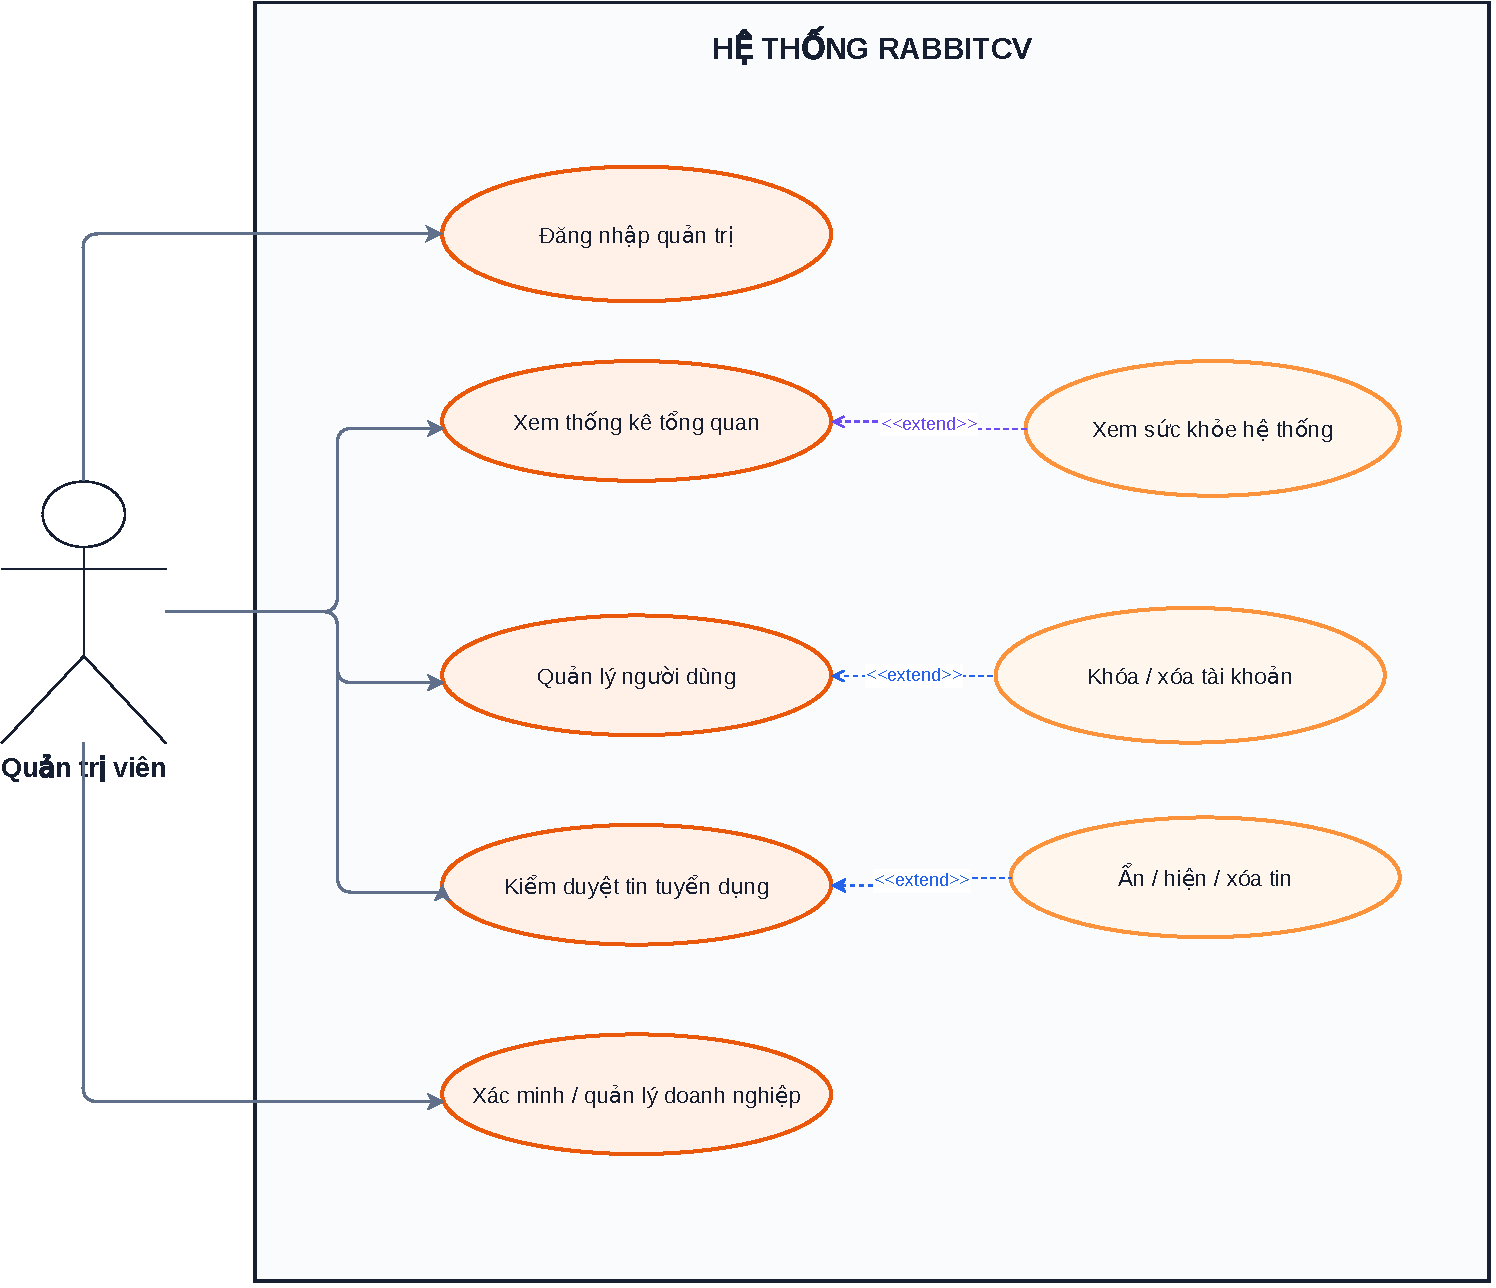
\includegraphics[
        width=0.85\linewidth,
        height=0.50\textheight,
        keepaspectratio
    ]{img/Admin-usecase.pdf}
    \caption{Lược đồ usecase phân hệ Quản trị viên}
    \label{fig:uc-admin-management}
\end{figure}

\begin{table}[H]
    \centering
    \small
    \renewcommand{\arraystretch}{1.0}
    \begin{tabularx}{\textwidth}{|
        >{\bfseries\raggedright\arraybackslash}p{3.2cm}|Y|}
        \hline

        Usecase ID & CV-5.1 \\ \hline

        Tên use case & Xem thống kê tổng quan \\ \hline

        Đối tượng & Quản trị viên \\ \hline

        Mô tả & Cho phép quản trị viên xem các chỉ số thống kê về hoạt động toàn bộ hệ thống và giám sát trạng thái vận hành của hệ thống \\ \hline

        Tiền điều kiện &
        \parbox[t]{\hsize}{
            1. Quản trị viên đã đăng nhập thành công vào hệ thống.\par
            2. Quản trị viên đang ở giao diện trang quản trị.
        } \\
        \hline

        Hậu điều kiện & Quản trị viên xem được số liệu tổng hợp và trạng thái vận hành tại thời điểm hệ thống thực hiện truy vấn \\ \hline

        Luồng thực hiện chính &
        \parbox[t]{\hsize}{
            1.\ Quản trị viên chọn mục "Tổng quan"\\
            2.\ Hệ thống truy vấn cơ sở dữ liệu và hiển thị các chỉ số thống kê, biểu đồ trực quan hóa số liệu
        }\\
        \hline

        Luồng thực hiện phụ &Không có\\
        \hline

        Lỗi &
        \parbox[t]{\hsize}{
            E1. Tài khoản không có vai trò Quản trị viên\\
            E2. Hệ thống đang bảo trì
        }\\
        \hline
    \end{tabularx}

    \caption{Use case CV-5.1: Xem thống kê tổng quan}
    \label{tab:usecase-cv51}
\end{table}

\begin{table}[H]
    \centering
    \small
    \renewcommand{\arraystretch}{1.0}
    \begin{tabularx}{\textwidth}{|
        >{\bfseries\raggedright\arraybackslash}p{3.2cm}|Y|}
        \hline

        Usecase ID & CV-5.2 \\ \hline

        Tên use case & Quản lý người dùng \\ \hline

        Đối tượng & Quản trị viên \\ \hline

        Mô tả & Cho phép quản trị viên tra cứu người dùng, khóa tài khoản vi phạm hoặc vô hiệu hóa tài khoản bằng thao tác xóa \\ \hline

        Tiền điều kiện &
        \parbox[t]{\hsize}{
            1. Quản trị viên đã đăng nhập thành công vào hệ thống.\par
            2. Quản trị viên đang ở giao diện quản trị hệ thống.
        } \\
        \hline

        Hậu điều kiện & Cập nhật trạng thái hoạt động của người dùng thành công \\ \hline

        Luồng thực hiện chính &
        \parbox[t]{\hsize}{
            1.\ Quản trị viên chọn mục "Quản lý người dùng"\\
            2.\ Hệ thống hiển thị danh sách người dùng\\
            3.\ Quản trị viên chọn tài khoản cần xử lý và thực hiện khóa hoặc xác nhận xóa tài khoản\\
            4.\ Hệ thống kiểm tra quyền và không cho phép xử lý chính tài khoản đang dùng; khóa hoặc vô hiệu hóa tài khoản theo thao tác đã chọn, giữ dữ liệu lịch sử ứng tuyển và hiển thị kết quả
        }\\
        \hline

        Luồng thực hiện phụ & Quản trị viên sử dụng từ khóa để lọc danh sách và xem thông tin người dùng trước khi xử lý \\
        \hline

        Lỗi &
        \parbox[t]{\hsize}{
            E1. Tài khoản thực hiện không có quyền Quản trị viên hệ thống\\
            E2. Không tìm thấy tài khoản người dùng cần thao tác\\
            E3. Quản trị viên yêu cầu khóa hoặc xóa tài khoản đang dùng để thực hiện thao tác\\
            E4. Máy chủ không cập nhật được tài khoản
        }\\
        \hline

    \end{tabularx}

    \caption{Use case CV-5.2: Quản lý người dùng}
    \label{tab:usecase-cv52}
\end{table}

\begin{table}[H]
    \centering
    \small
    \renewcommand{\arraystretch}{1.0}
    \begin{tabularx}{\textwidth}{|
        >{\bfseries\raggedright\arraybackslash}p{3.2cm}|Y|}
        \hline

        Usecase ID & CV-5.3 \\ \hline

        Tên use case & Quản lý doanh nghiệp \\ \hline

        Đối tượng & Quản trị viên \\ \hline

        Mô tả & Cho phép quản trị viên xét duyệt tài khoản doanh nghiệp, quản lý trạng thái xác minh và khóa hoặc mở khóa tài khoản doanh nghiệp \\ \hline

        Tiền điều kiện &
        \parbox[t]{\hsize}{
            1. Quản trị viên đã đăng nhập thành công vào hệ thống.\par
            2. Quản trị viên đang ở giao diện quản lý doanh nghiệp.
        } \\
        \hline

        Hậu điều kiện & Trạng thái phê duyệt, xác minh hoặc khóa tài khoản doanh nghiệp được cập nhật theo thao tác của quản trị viên \\ \hline

        Luồng thực hiện chính &
        \parbox[t]{\hsize}{
            1.\ Quản trị viên chọn mục "Quản lý doanh nghiệp"\\
            2.\ Hệ thống hiển thị danh sách các doanh nghiệp\\
            3.\ Quản trị viên mở chi tiết doanh nghiệp và kiểm tra thông tin đăng ký\\
            4.\ Quản trị viên chọn duyệt tài khoản hoặc từ chối và nhập lý do; hệ thống cập nhật kết quả xét duyệt tài khoản
        }\\
        \hline

        Luồng thực hiện phụ &
        \parbox[t]{\hsize}{
            1.\ Với doanh nghiệp đã được phê duyệt và không bị khóa, quản trị viên có thể xác minh hoặc thu hồi xác minh; trạng thái này quyết định chính sách xét duyệt tin tuyển dụng\\
            2.\ Quản trị viên có thể khóa hoặc mở khóa tài khoản doanh nghiệp\\
            3.\ Quản trị viên có thể tạo tài khoản doanh nghiệp mới; tài khoản được tạo có trạng thái đã phê duyệt và trạng thái xác minh theo lựa chọn
        }\\
        \hline

        Lỗi &
        \parbox[t]{\hsize}{
            E1. Tài khoản thực hiện không có quyền Quản trị viên hệ thống\\
            E2. Không tìm thấy thông tin doanh nghiệp yêu cầu\\
            E3. Thiếu lý do từ chối hoặc yêu cầu xác minh doanh nghiệp chưa được duyệt hay đang bị khóa\\
            E4. Thông tin tạo tài khoản không hợp lệ, tên đăng nhập hoặc email đã tồn tại\\
            E5. Máy chủ không lưu được thay đổi
        }\\
        \hline

    \end{tabularx}

    \caption{Use case CV-5.3: Quản lý doanh nghiệp}
    \label{tab:usecase-cv53}
\end{table}

\section{Lược đồ hoạt động (Activity Diagram)}
\subsection{Đăng ký, đăng nhập và quên mật khẩu}
\begin{figure}[H]
    \centering
    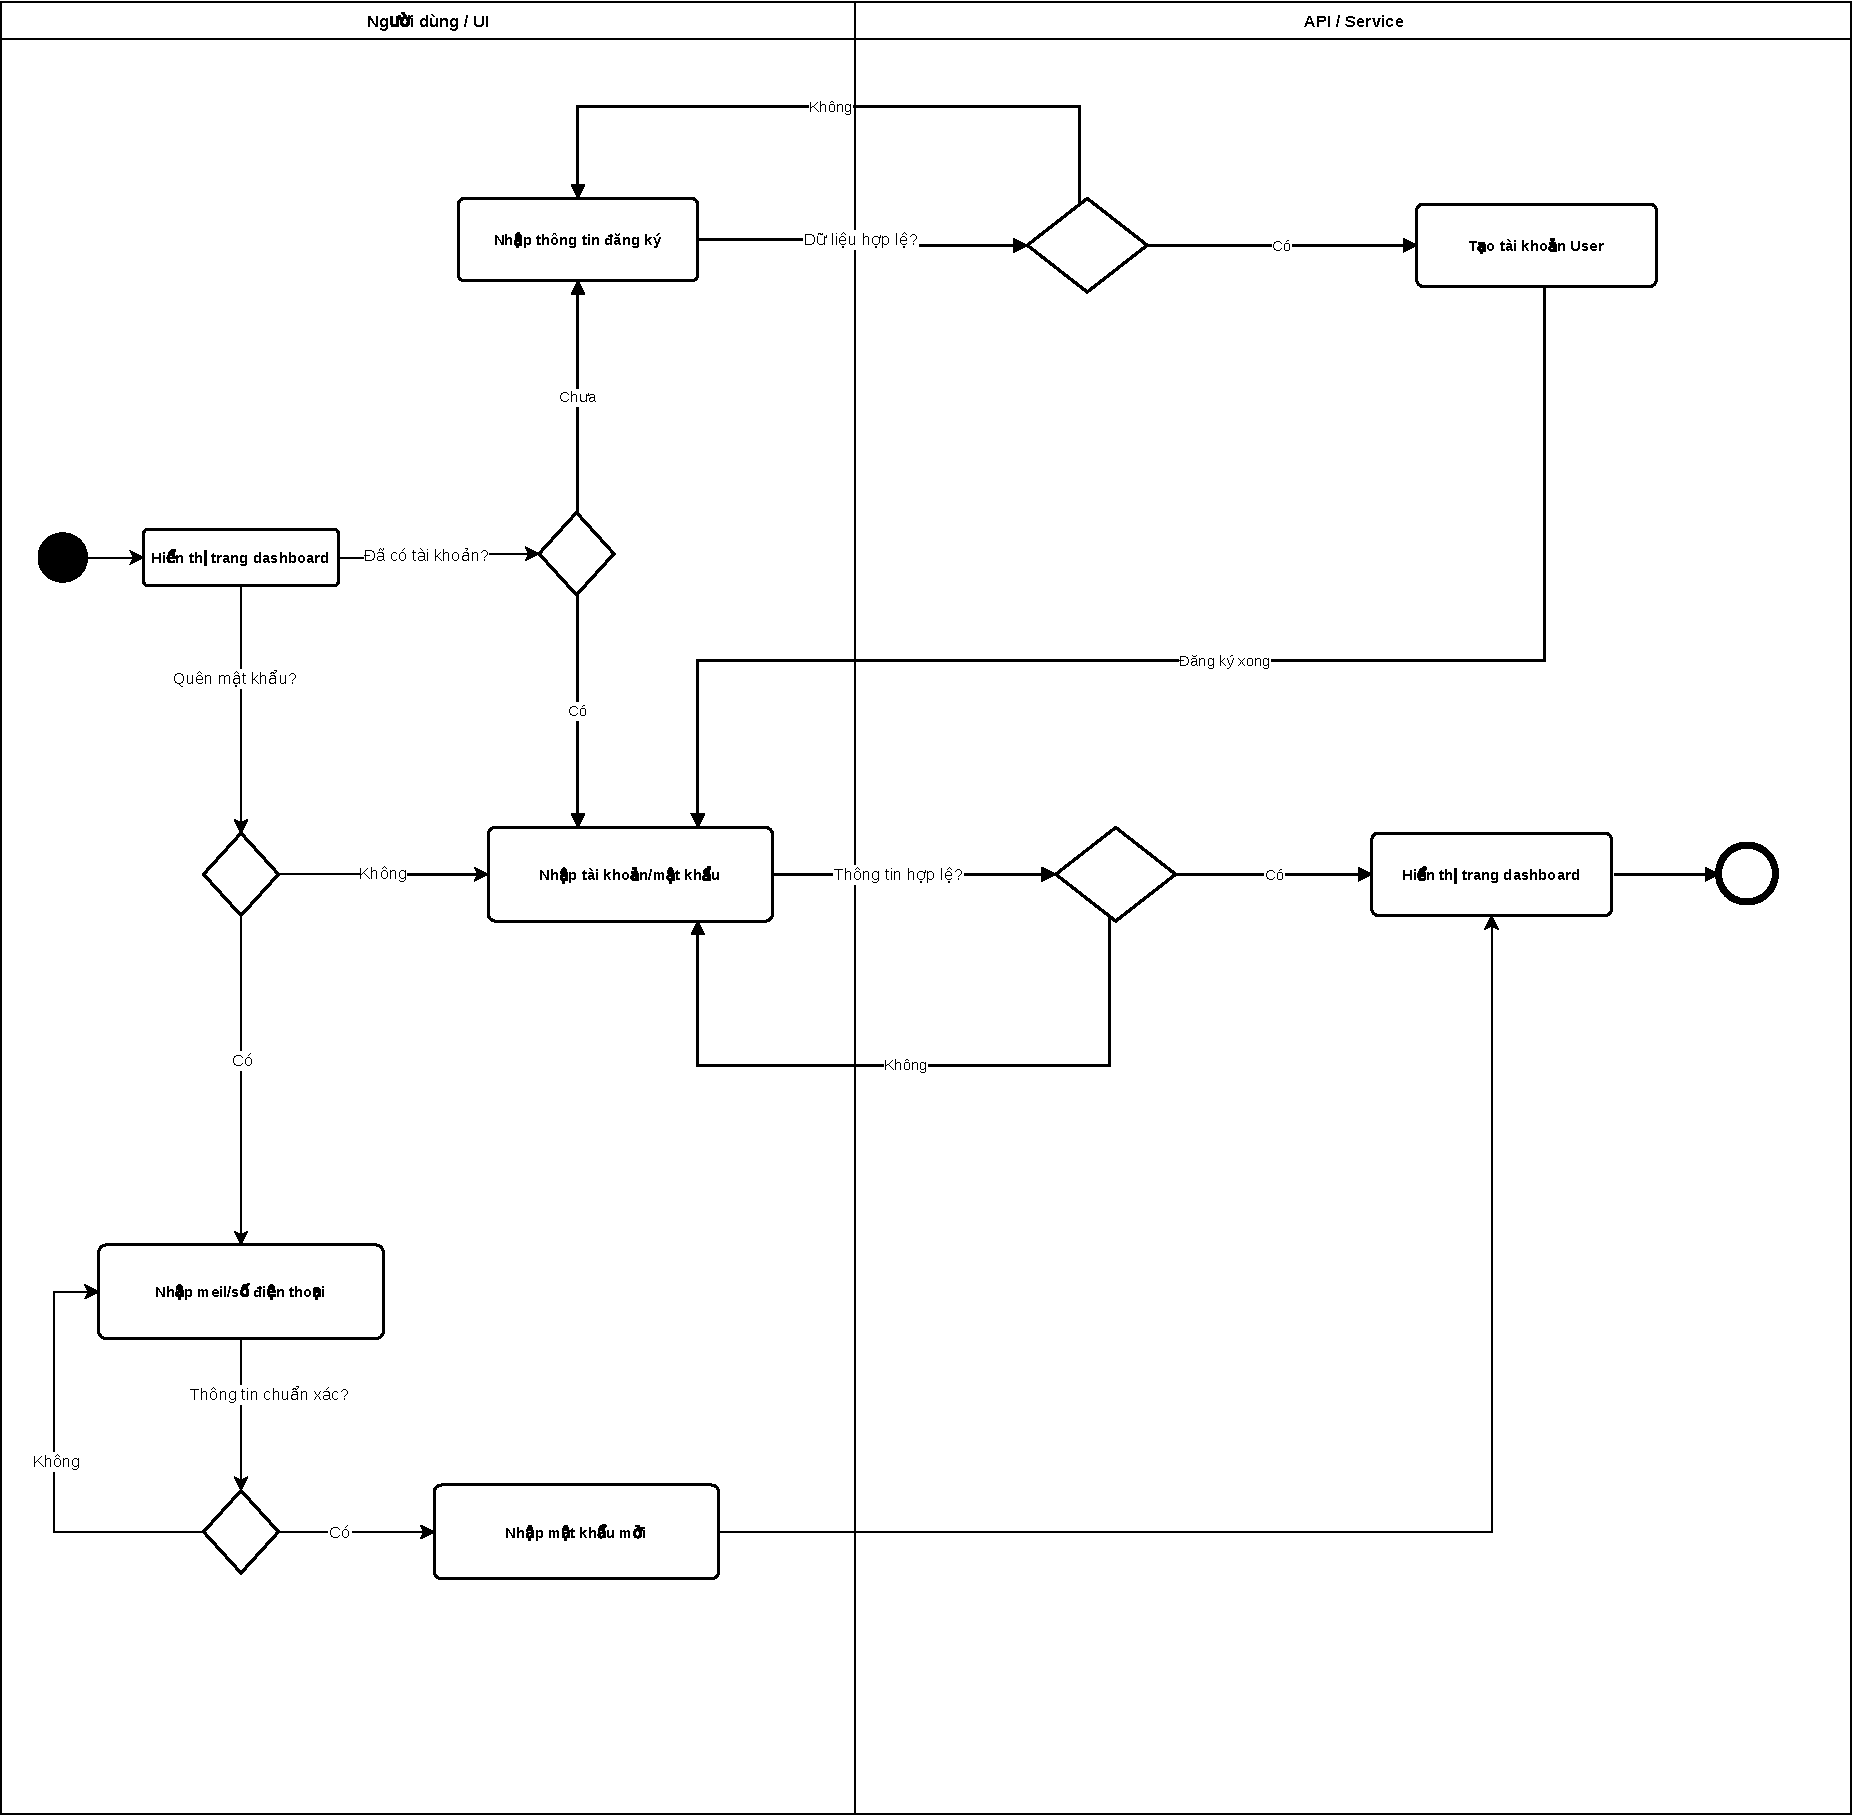
\includegraphics[
        width=0.9\linewidth,
        height=0.75\textheight,
        keepaspectratio
    ]{img/ActivityDiagram_1.pdf}
    \caption{Lược đồ hoạt động: Đăng ký, đăng nhập và quên mật khẩu}
    \label{fig:activity-diagram-registration-login-password-reset}
\end{figure}

Sơ đồ trong Hình~\ref{fig:activity-diagram-registration-login-password-reset} thể hiện quy trình xử lý của hệ thống khi thực hiện chức năng đăng ký, đăng nhập và quên mật khẩu. Các bước xử lý bao gồm:

\begin{itemize}
    \item \textbf{Đăng ký:} Khi người dùng chọn chức năng đăng ký, hệ thống hiển thị biểu mẫu đăng ký. Sau khi người dùng nhập thông tin, hệ thống tiến hành kiểm tra tính hợp lệ. Nếu dữ liệu hợp lệ, hệ thống tạo tài khoản mới vào cơ sở dữ liệu và hiển thị thông báo đăng ký thành công.
    \item \textbf{Đăng nhập:} Khi người dùng chọn chức năng đăng nhập, hệ thống hiển thị biểu mẫu đăng nhập. Sau khi người dùng nhập thông tin tài khoản và mật khẩu, hệ thống tiến hành xác thực danh tính. Nếu thông tin chính xác, hệ thống khởi tạo phiên làm việc và hiển thị thông báo đăng nhập thành công.
    \item \textbf{Quên mật khẩu:} Khi người dùng chọn chức năng quên mật khẩu, hệ thống hiển thị biểu mẫu nhập địa chỉ email. Sau khi xác nhận email tồn tại trong hệ thống, hệ thống gửi email chứa liên kết đặt lại mật khẩu và hiển thị thông báo hướng dẫn cho người dùng.
\end{itemize}

\subsection{Quản lý CV}

\begin{figure}[H]
    \centering
    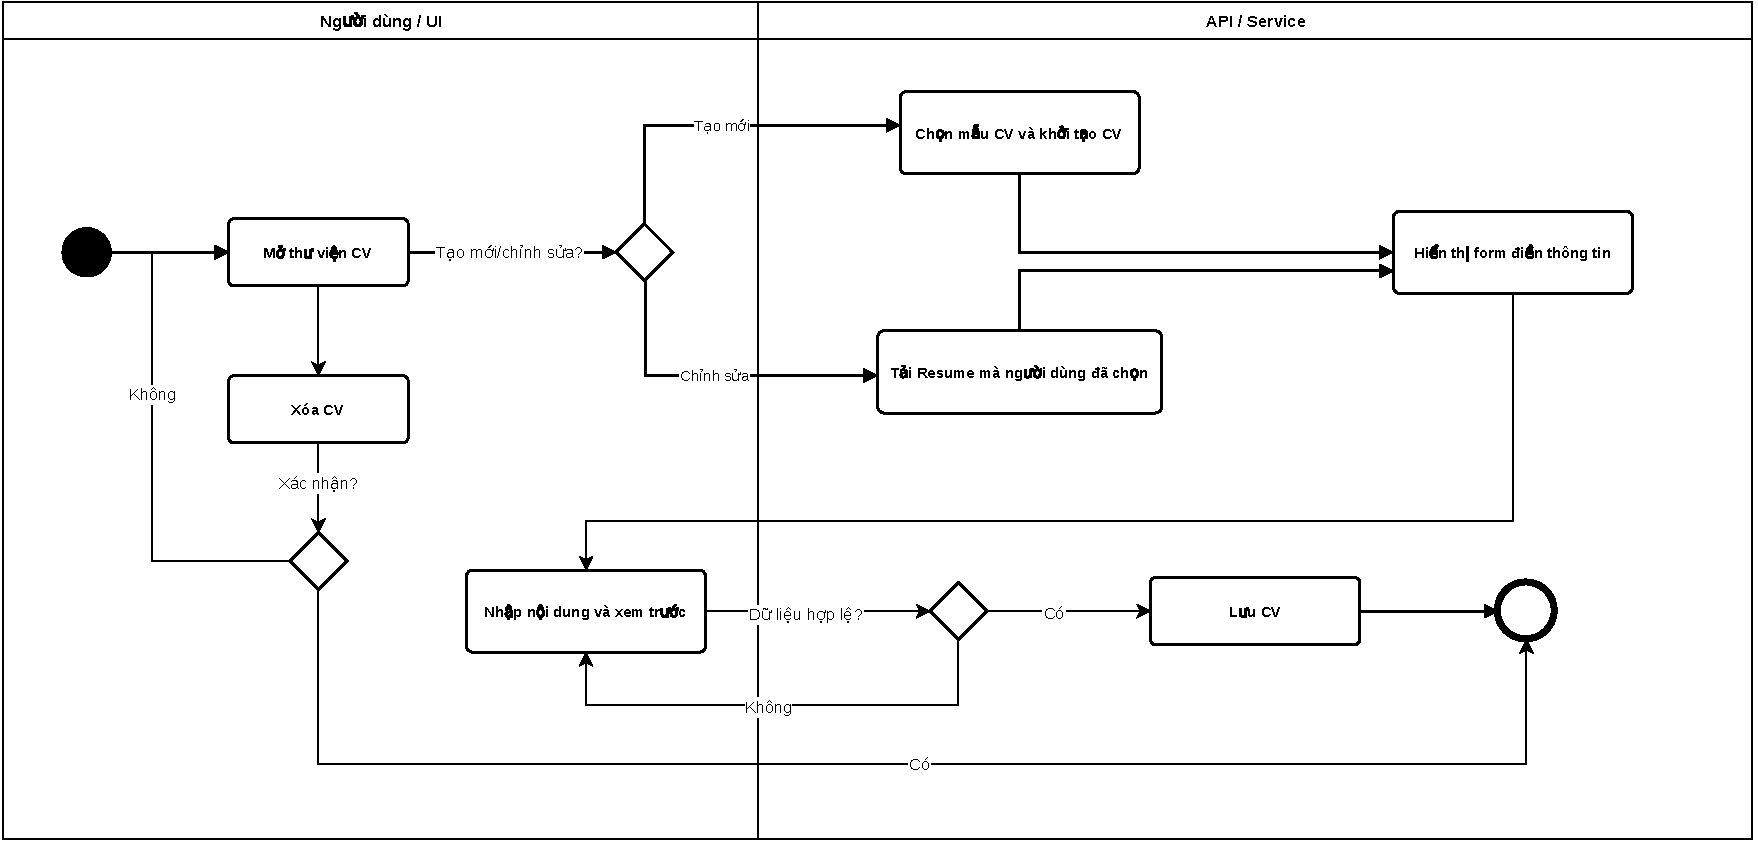
\includegraphics[
        width=0.9\linewidth,
        height=0.75\textheight,
        keepaspectratio
    ]{img/ActivityDiagram_CV.pdf}
    \caption{Lược đồ hoạt động: Quản lý CV}
    \label{fig:activity-diagram-cv-management}
\end{figure}

Sơ đồ trong Hình~\ref{fig:activity-diagram-cv-management} thể hiện quy trình xử lý của hệ thống khi thực hiện chức năng quản lý CV bao gồm: tạo mới CV, chỉnh sửa CV và xóa CV. Nếu người dùng chọn chức năng tạo mới CV, hệ thống sẽ yêu cầu người dùng chọn mẫu giao diện trước khi chuyển đến trình soạn thảo. Sau khi người dùng nhập thông tin và xác nhận lưu, hệ thống sẽ ghi nhận dữ liệu vào cơ sở dữ liệu và hiển thị thông báo thành công. Đối với chức năng chỉnh sửa CV, hệ thống tải dữ liệu hiện có lên giao diện soạn thảo; sau khi người dùng cập nhật, hệ thống ghi đè dữ liệu mới và thông báo hoàn tất. Chức năng xóa CV được hỗ trợ trực tiếp tại trang quản lý danh sách giúp thao tác thuận tiện và nhanh chóng.

\subsection{Tìm kiếm việc làm}

\begin{figure}[H]
    \centering
    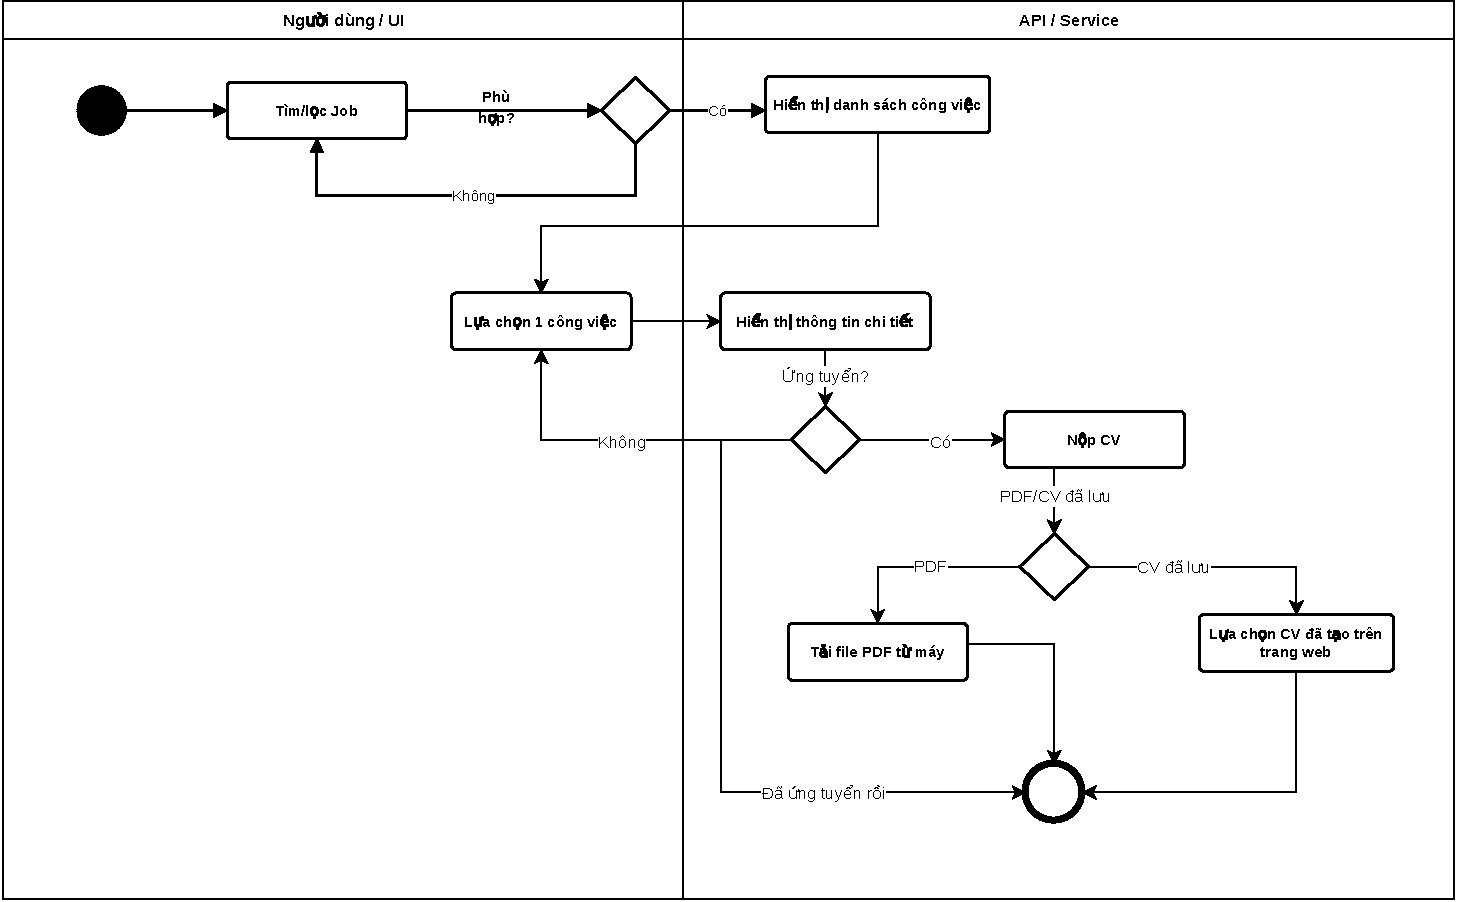
\includegraphics[
        width=0.9\linewidth,
        height=0.75\textheight,
        keepaspectratio
    ]{img/ActivityDiagram_Jobs.pdf}
    \caption{Lược đồ hoạt động: Tìm kiếm việc làm}
    \label{fig:activity-diagram-job-search}
\end{figure}

Sơ đồ trong Hình~\ref{fig:activity-diagram-job-search} thể hiện quy trình tìm kiếm việc làm và lọc tin tuyển dụng. Khi người dùng truy cập trang việc làm, hệ thống hiển thị danh sách các bài đăng đang hoạt động kèm thanh công cụ tìm kiếm. Hệ thống hỗ trợ đa dạng các bộ lọc như chức danh, mức lương, địa điểm làm việc, số năm kinh nghiệm... Khi người dùng áp dụng bộ lọc hoặc nhập từ khóa tìm kiếm, hệ thống sẽ truy vấn cơ sở dữ liệu và hiển thị danh sách công việc thỏa mãn tiêu chí. Trường hợp không tìm thấy kết quả phù hợp, hệ thống sẽ phản hồi thông báo tương ứng.

\subsection{Quản lý tin tuyển dụng}

\begin{figure}[H]
    \centering
    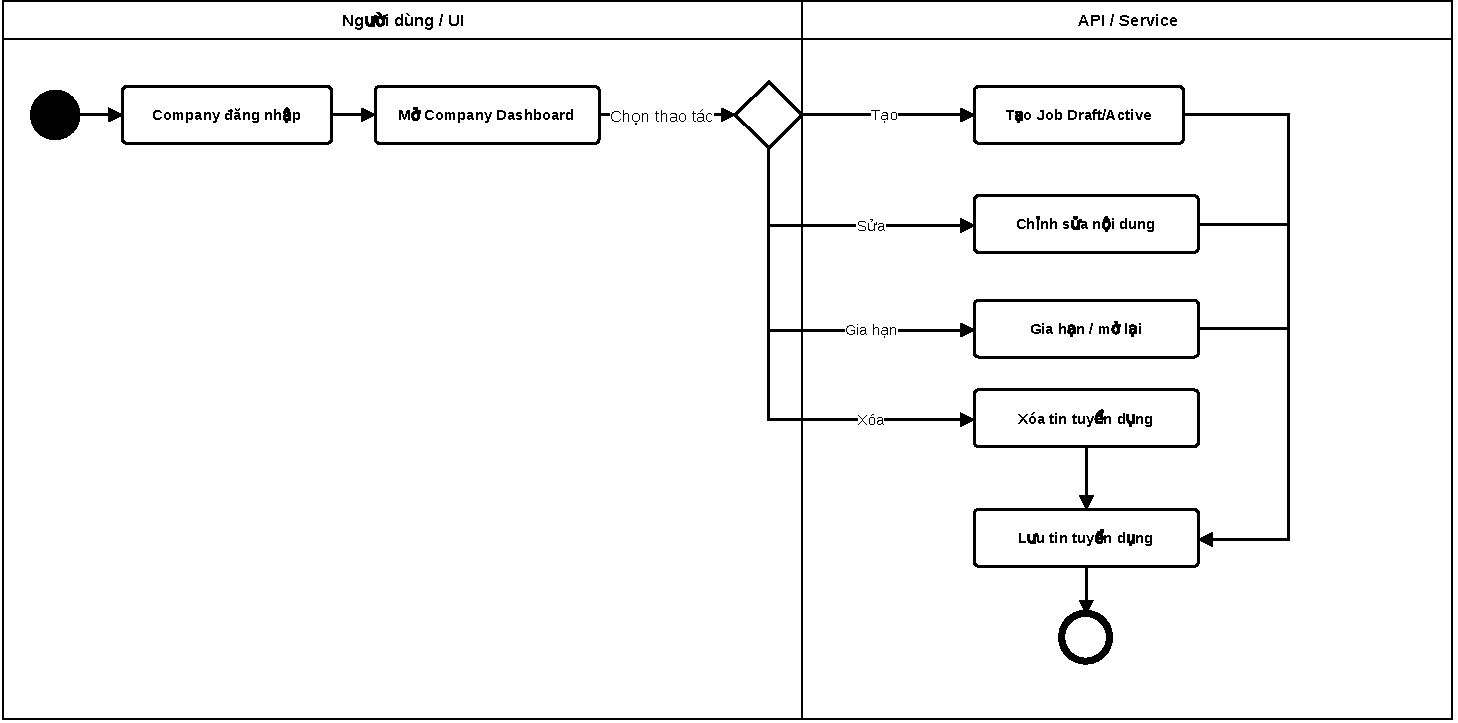
\includegraphics[
        width=0.92\linewidth,
        height=0.5\textheight,
        keepaspectratio
    ]{img/ActivityDiagram_JobsPostingManagement.pdf}
    \caption{Lược đồ hoạt động: Quản lý tin tuyển dụng}
    \label{fig:activity-diagram-job-posting-management}
\end{figure}

Sơ đồ trong Hình~\ref{fig:activity-diagram-job-posting-management} thể hiện quy trình xử lý của hệ thống khi thực hiện chức năng quản lý tin tuyển dụng phía doanh nghiệp bao gồm:

\begin{itemize}
    \item \textbf{Tạo mới tin tuyển dụng:} Khi doanh nghiệp chọn tạo tin tuyển dụng, hệ thống hiển thị biểu mẫu nhập liệu. Sau khi người dùng điền thông tin, hệ thống tiến hành kiểm tra tính hợp lệ của dữ liệu. Doanh nghiệp có thể lựa chọn lưu nháp (Draft) nếu chưa hoàn thiện nội dung hoặc chọn đăng tuyển chính thức (Active) để công khai bài đăng trên hệ thống.
    \item \textbf{Chỉnh sửa tin tuyển dụng:} Doanh nghiệp chọn tin tuyển dụng cần cập nhật, hệ thống hiển thị lại toàn bộ nội dung hiện có để chỉnh sửa. Dữ liệu mới sau khi kiểm tra hợp lệ sẽ được cập nhật vào cơ sở dữ liệu kèm thông báo thành công.
    \item \textbf{Gia hạn hoặc mở lại tin tuyển dụng:} Doanh nghiệp có thể gia hạn thời gian nhận hồ sơ hoặc mở lại tin đã đóng; hệ thống cập nhật lại thời hạn kết thúc và trạng thái hoạt động tương ứng.
    \item \textbf{Xóa tin tuyển dụng:} Doanh nghiệp gửi yêu cầu xóa bài đăng, hệ thống hiển thị hộp thoại xác nhận. Khi được xác nhận, hệ thống tiến hành xóa tin khỏi cơ sở dữ liệu và cập nhật lại danh sách quản lý.
\end{itemize}

\subsection{Cập nhật trạng thái hồ sơ ứng tuyển}

\begin{figure}[H]
    \centering
    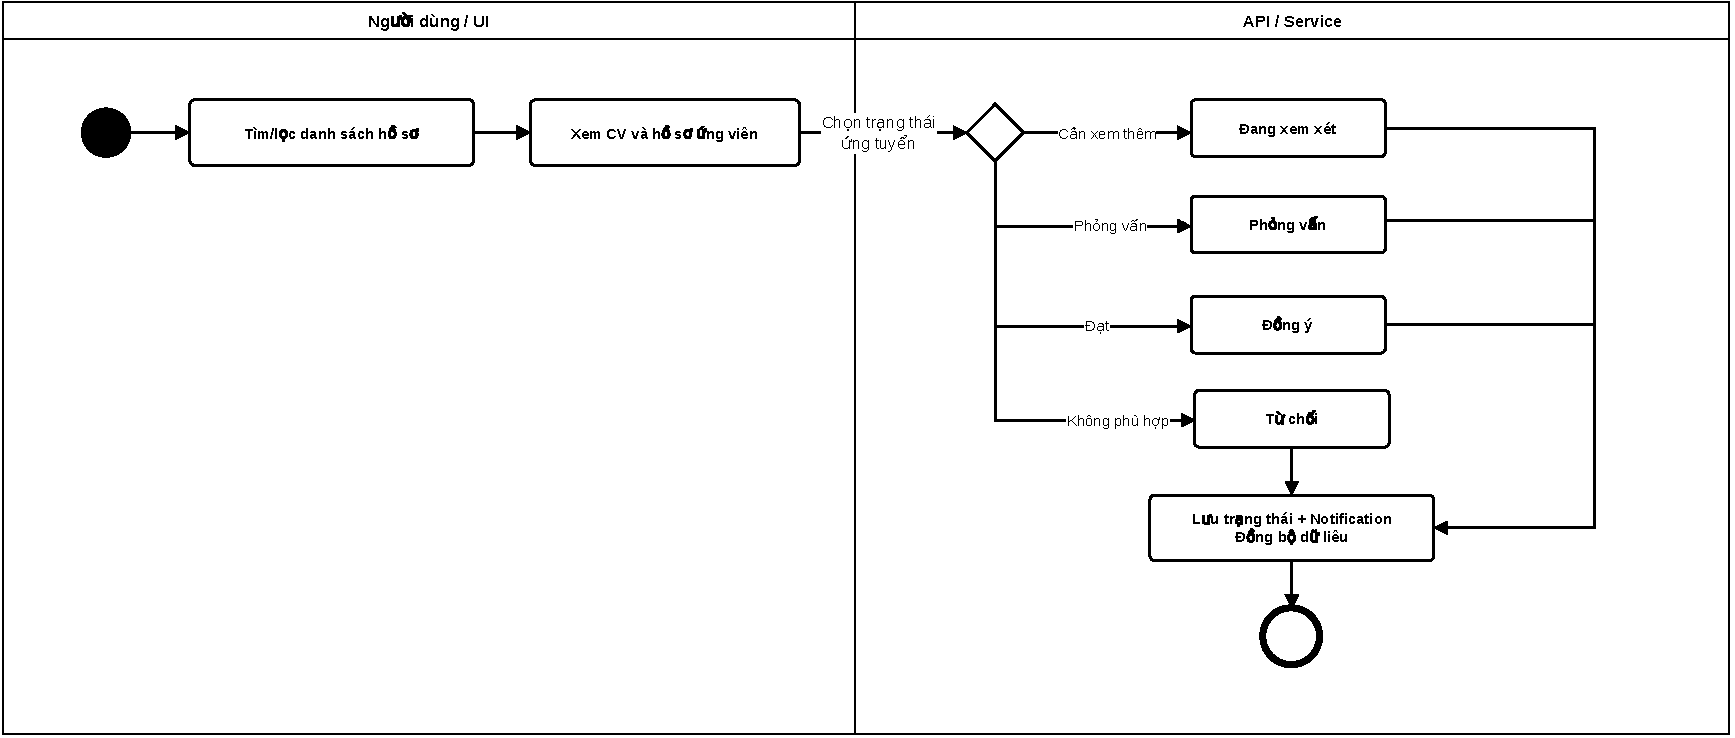
\includegraphics[
        width=0.88\linewidth,
        height=0.6\textheight,
        keepaspectratio
    ]{img/ActivityDiagram_StatusUpdate.pdf}
    \caption{Lược đồ hoạt động: Cập nhật trạng thái hồ sơ ứng tuyển}
    \label{fig:activity-diagram-status-update}
\end{figure}

Sơ đồ trong Hình~\ref{fig:activity-diagram-status-update} thể hiện quy trình xem xét và cập nhật trạng thái hồ sơ ứng tuyển từ phía nhà tuyển dụng. Khi doanh nghiệp truy cập danh sách ứng viên của một tin tuyển dụng, hệ thống hiển thị thông tin tóm tắt và cho phép xem chi tiết từng hồ sơ (bao gồm CV đính kèm). Doanh nghiệp có thể chuyển đổi trạng thái hồ sơ sang các mốc xét duyệt: \textbf{Đang xem xét}, \textbf{Phỏng vấn}, \textbf{Đồng ý} hoặc \textbf{Từ chối}. Sau khi trạng thái mới được lưu vào cơ sở dữ liệu, hệ thống tự động phát thông báo nghiệp vụ đến tài khoản ứng viên.

\subsection{Phỏng vấn với AI}

\begin{figure}[H]
    \centering
    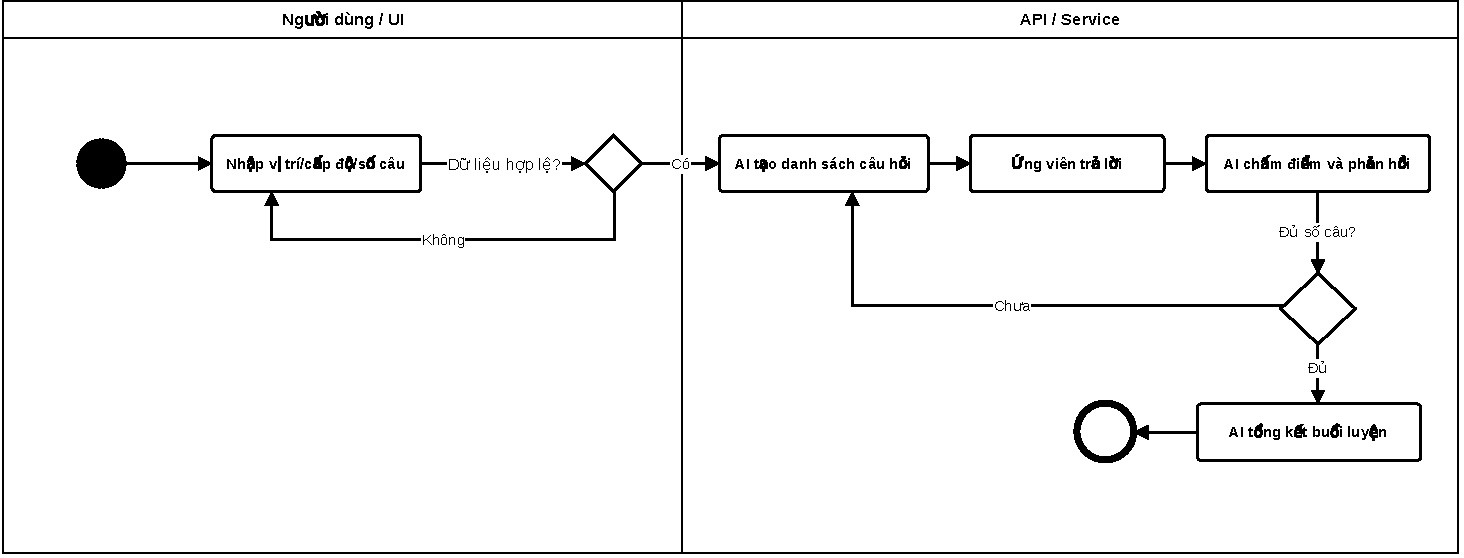
\includegraphics[
        width=0.88\linewidth,
        height=0.6\textheight,
        keepaspectratio
    ]{img/ActivityDiagram_AIInterview.pdf}
    \caption{Lược đồ hoạt động: Phỏng vấn với AI}
    \label{fig:activity-diagram-ai-interview}
\end{figure}

Sơ đồ trong Hình~\ref{fig:activity-diagram-ai-interview} thể hiện quy trình mô phỏng phỏng vấn thông minh giữa ứng viên và trợ lý AI. Trước khi bắt đầu, ứng viên chọn vị trí công việc, cấp độ chuyên môn, hình thức phỏng vấn và số lượng câu hỏi mong muốn. Dựa trên các thông số này, hệ thống gửi yêu cầu để AI sinh bộ câu hỏi tương ứng và hiển thị lần lượt từng câu. Sau khi ứng viên nhập câu trả lời, hệ thống gửi dữ liệu đến AI để nhận xét tức thời và chuyển sang câu tiếp theo. Khi hoàn thành toàn bộ câu hỏi, hệ thống tổng kết buổi phỏng vấn bằng bảng đánh giá toàn diện gồm điểm số tổng thể, điểm theo kỹ năng và gợi ý chi tiết để ứng viên cải thiện.

\subsection{Quản trị viên}

\begin{figure}[H]
    \centering
    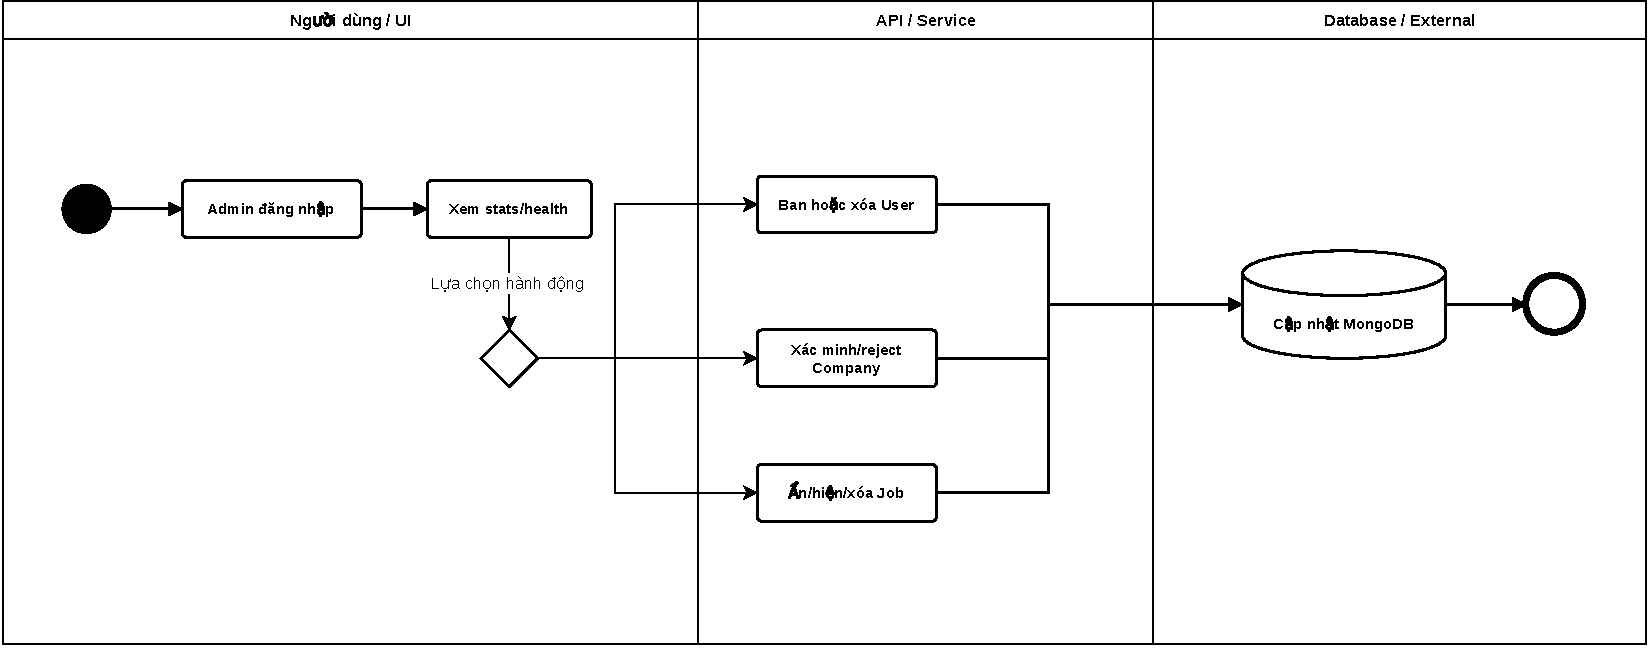
\includegraphics[
        width=0.92\linewidth,
        height=0.5\textheight,
        keepaspectratio
    ]{img/ActivityDiagram_AdminManagement.pdf}
    \caption{Lược đồ hoạt động: Quản trị viên}
    \label{fig:activity-diagram-admin-management}
\end{figure}

Sơ đồ trong Hình~\ref{fig:activity-diagram-admin-management} thể hiện quy trình xử lý của hệ thống đối với các tác vụ thuộc phân hệ Quản trị viên:

\begin{itemize}
    \item \textbf{Đăng nhập và giám sát hệ thống:} Quản trị viên đăng nhập vào hệ thống bằng tài khoản đặc quyền. Sau khi xác thực thành công, bảng điều khiển quản trị hiển thị các số liệu thống kê tổng quan về số lượng người dùng, doanh nghiệp, tin tuyển dụng, cũng như thông tin theo dõi sức khỏe hoạt động của hệ thống.
    \item \textbf{Các thao tác nghiệp vụ quản trị:}
    \begin{itemize}
        \item \textbf{Quản lý người dùng (Khóa hoặc xóa tài khoản):} Quản trị viên tra cứu danh sách tài khoản và thực hiện thao tác khóa tài khoản vi phạm chính sách hoặc xóa người dùng khi cần thiết.
        \item \textbf{Kiểm duyệt doanh nghiệp (Xác minh hoặc từ chối):} Quản trị viên thẩm định hồ sơ thông tin doanh nghiệp đăng ký mới nhằm xác thực tính hợp lệ hoặc từ chối phê duyệt đối với các hồ sơ không đạt chuẩn.
        \item \textbf{Kiểm duyệt tin tuyển dụng (Ẩn, hiện hoặc xóa bài đăng):} Quản trị viên kiểm tra nội dung các tin tuyển dụng trên hệ thống, chủ động ẩn bài đăng vi phạm, khôi phục hiển thị hoặc xóa bài đăng sai quy định.
    \end{itemize}
\end{itemize}

\section{Lược đồ tuần tự (Sequence Diagram)}

\subsection{Đăng ký, đăng nhập}

\begin{figure}[H]
    \centering
    \makebox[\linewidth][c]{%
        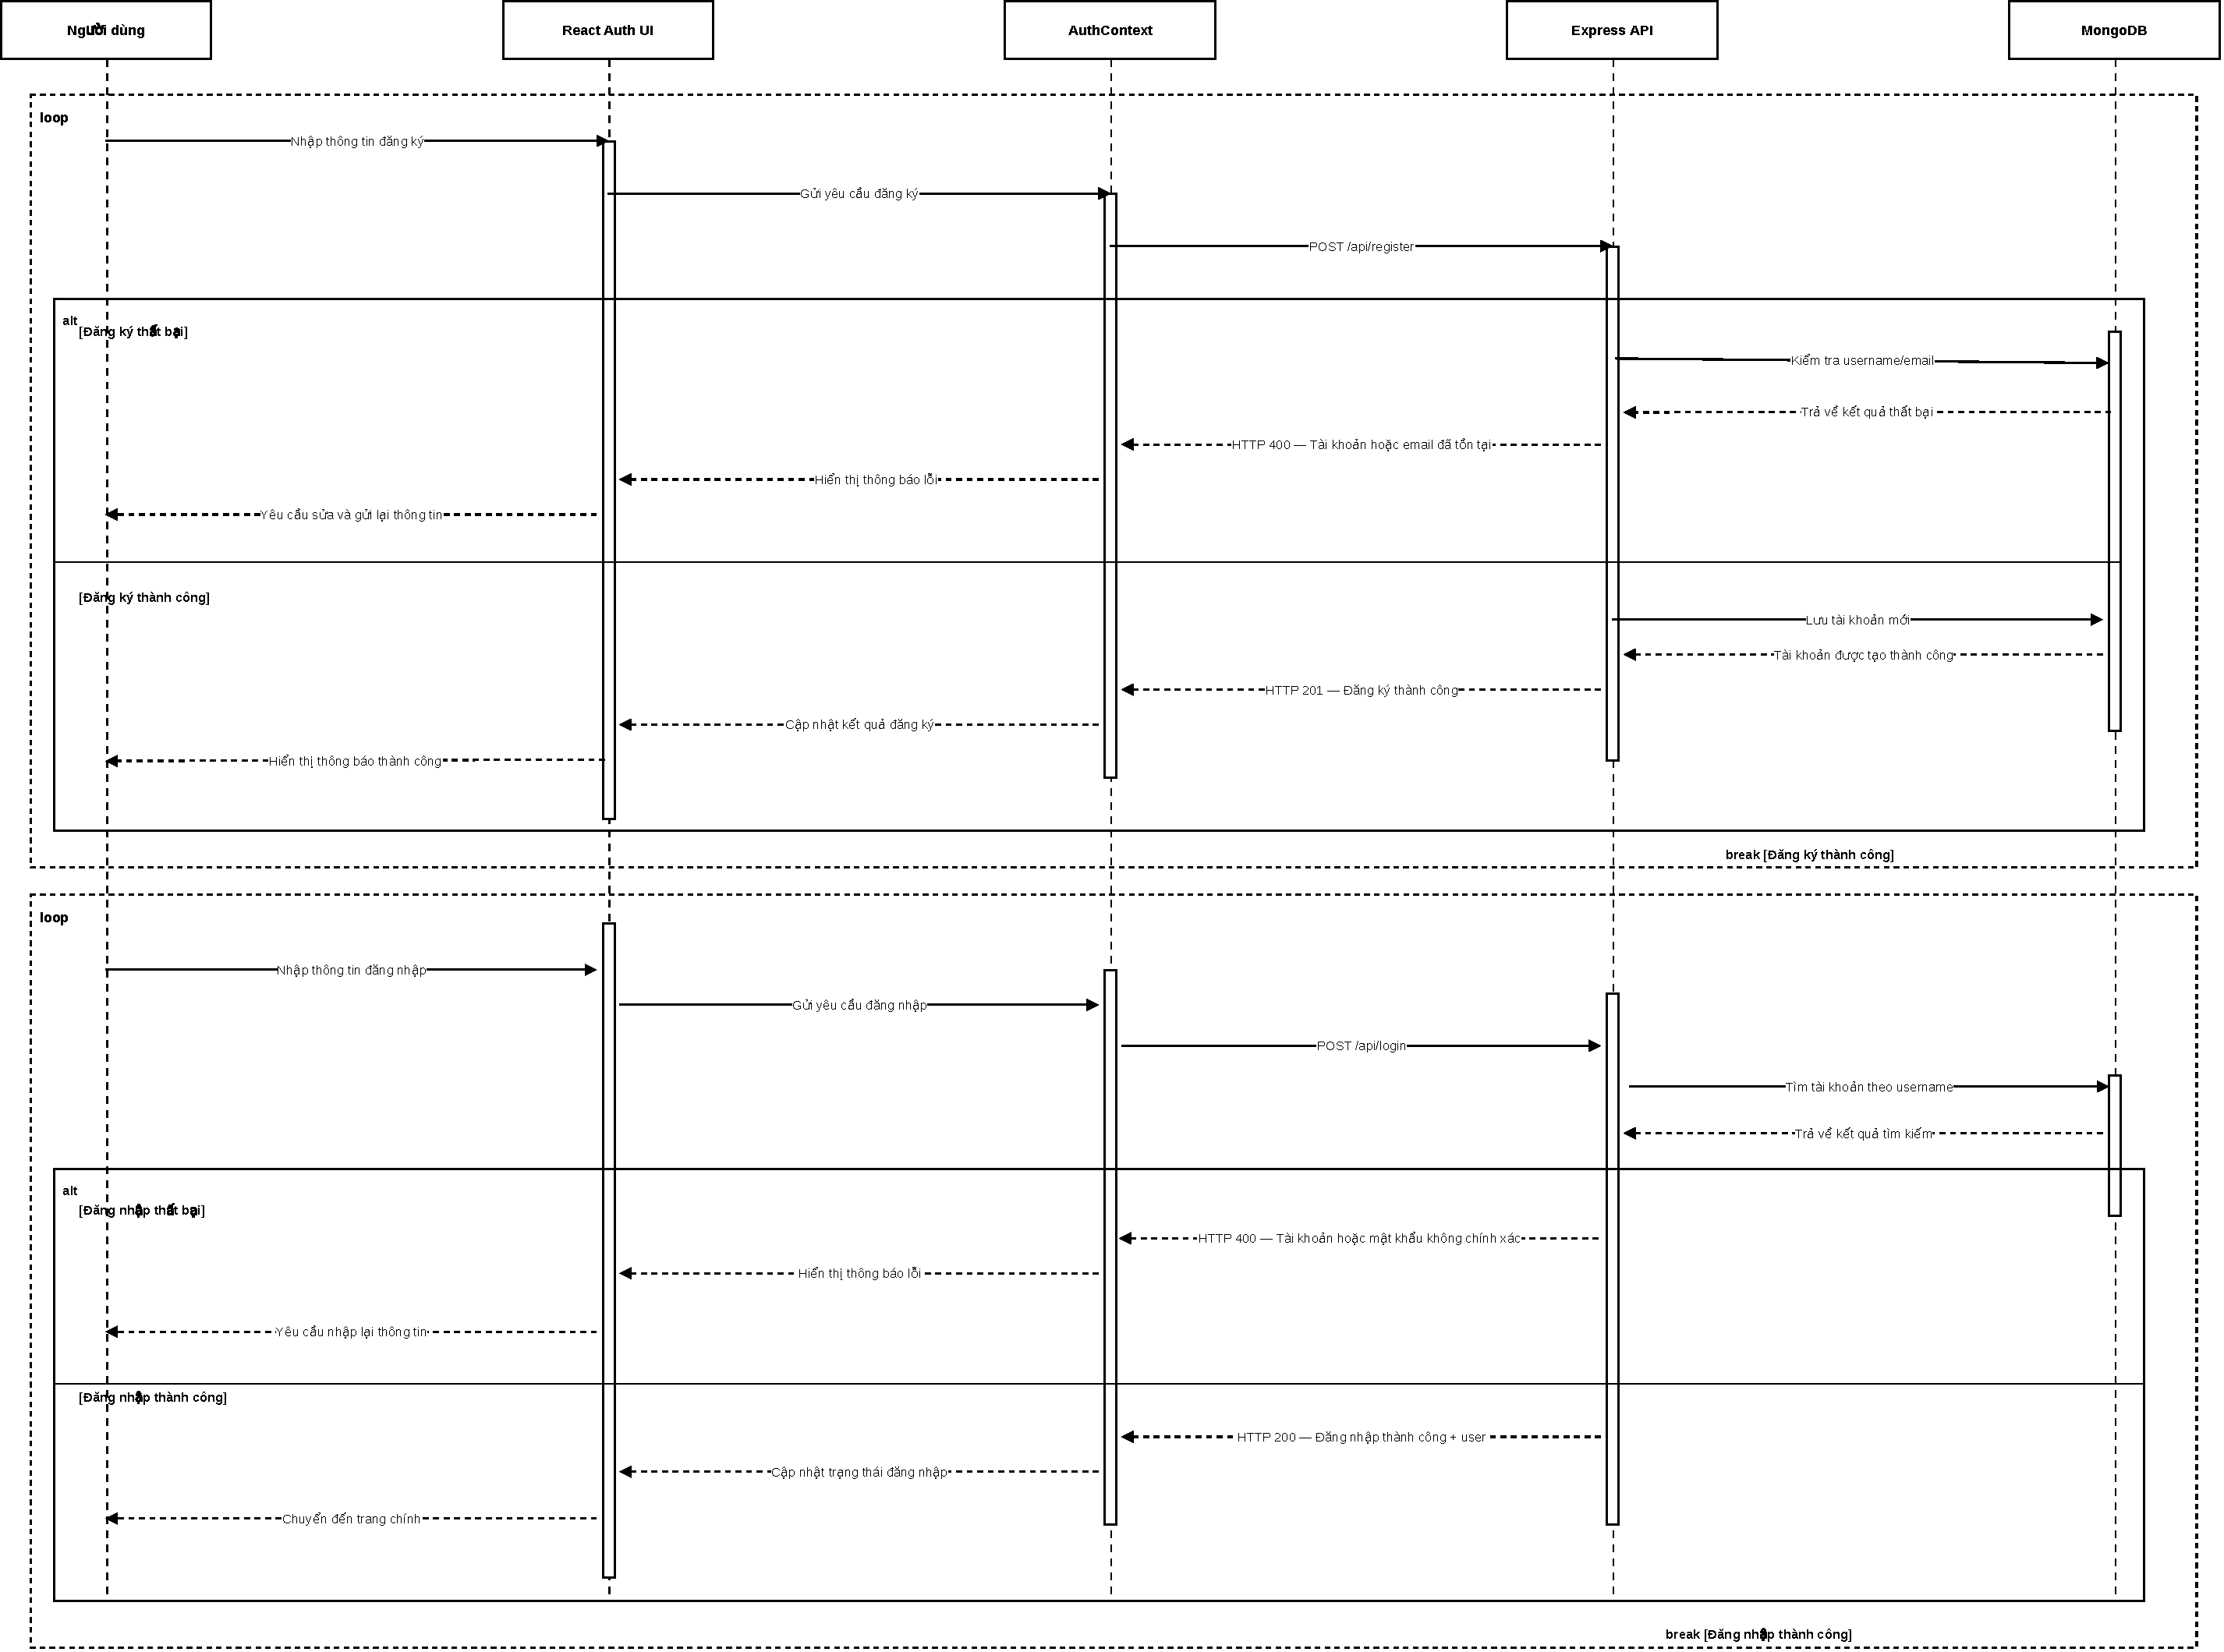
\includegraphics[
            width=1.1\linewidth,
            height=0.68\textheight,
            keepaspectratio
        ]{img/SequenceDiagram_LoginRegister.pdf}%
    }
    \caption{Lược đồ tuần tự: Đăng ký, đăng nhập}
    \label{fig:sequence-diagram-login-register}
\end{figure}

Lược đồ tuần tự trong Hình~\ref{fig:sequence-diagram-login-register} thể hiện quy trình xử lý của hoạt động đăng nhập và đăng ký. Để đăng nhập, người dùng nhập email (hoặc tên đăng nhập) và mật khẩu. Hệ thống tiến hành xác thực tài khoản; nếu thông tin chính xác, hệ thống khởi tạo JWT lưu vào Cookie và chuyển hướng người dùng đến giao diện tương ứng theo vai trò. Đối với hoạt động đăng ký, hệ thống yêu cầu cung cấp các thông tin bắt buộc gồm họ tên, email hợp lệ và mật khẩu. Mật khẩu được mã hóa an toàn bằng thuật toán băm (bcrypt) trước khi lưu trữ vào cơ sở dữ liệu.

\subsection{Quản lý CV}

\begin{figure}[H]
    \centering
    \makebox[\linewidth][c]{%
        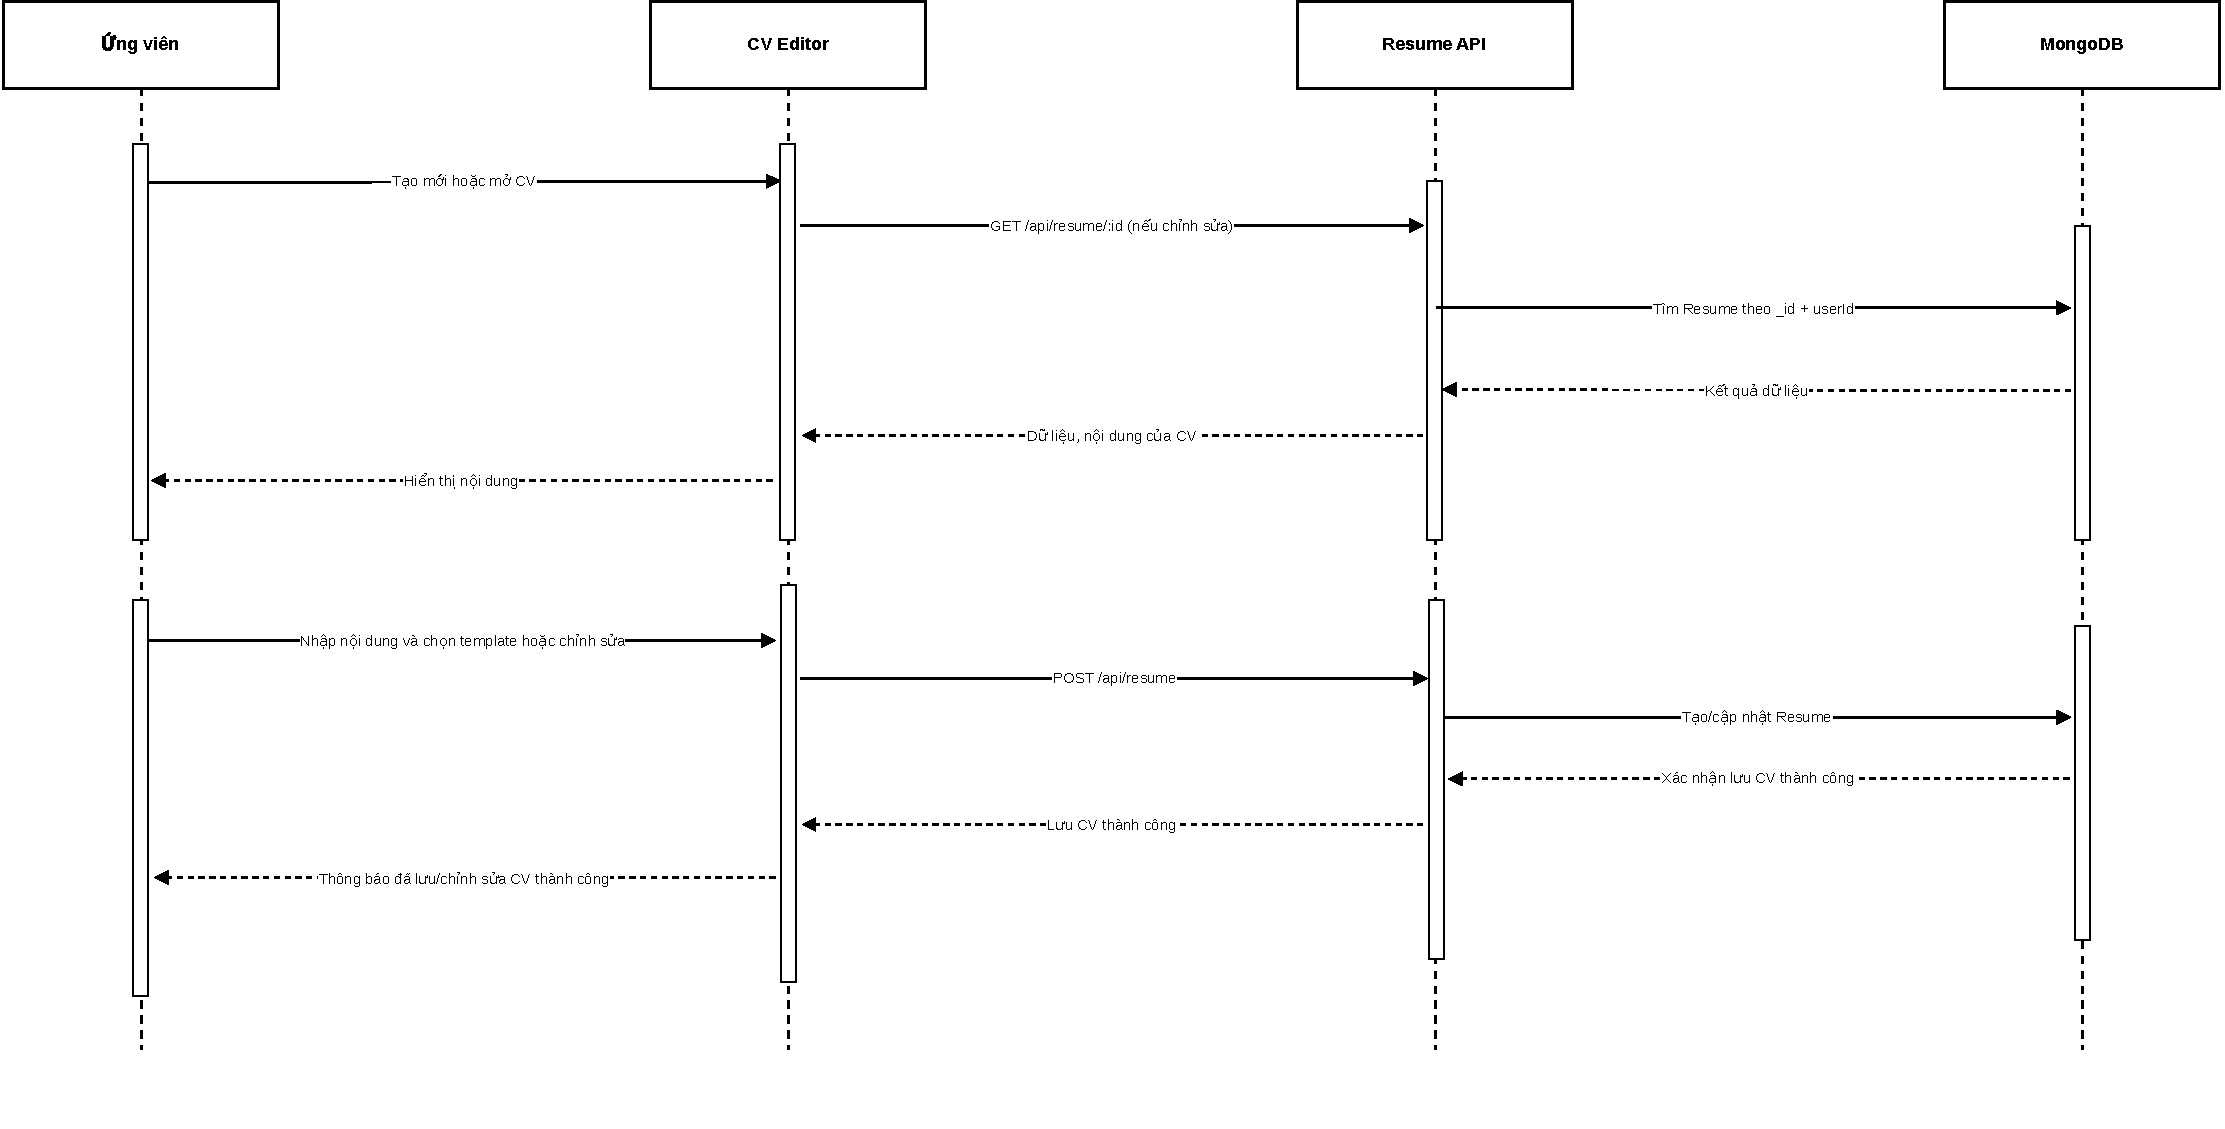
\includegraphics[
            width=1.12\linewidth,
            height=0.68\textheight,
            keepaspectratio
        ]{img/SequenceDiagram_CV.pdf}%
    }
    \caption{Lược đồ tuần tự: Quản lý CV}
    \label{fig:sequence-diagram-cv}
\end{figure}

Lược đồ tuần tự trong Hình~\ref{fig:sequence-diagram-cv} thể hiện quy trình khi ứng viên tạo mới, mở hoặc chỉnh sửa CV:

\begin{itemize}
    \item \textbf{Tạo mới CV:} Ứng viên chọn mẫu và tạo mới CV, hệ thống hiển thị biểu mẫu soạn thảo. Khi ứng viên hoàn thiện nội dung và nhấn lưu, hệ thống gửi dữ liệu đến backend để tạo tài liệu mới trong cơ sở dữ liệu MongoDB và phản hồi thông báo lưu thành công.
    \item \textbf{Mở CV:} Khi ứng viên chọn mở một CV đã lưu, hệ thống truy vấn cơ sở dữ liệu theo mã định danh của CV và xác thực quyền sở hữu của người dùng. Khi tìm thấy, hệ thống tải dữ liệu và hiển thị lên giao diện soạn thảo.
    \item \textbf{Chỉnh sửa và lưu CV:} Trong quá trình soạn thảo, ứng viên thay đổi nội dung các trường thông tin hoặc chuyển đổi template hiển thị và nhấn lưu. Hệ thống gửi yêu cầu cập nhật về backend, ghi đè thông tin mới vào MongoDB và thông báo kết quả cập nhật thành công cho ứng viên.
\end{itemize}

\subsection{Phỏng vấn với AI}

\begin{figure}[H]
    \centering
    \makebox[\linewidth][c]{%
        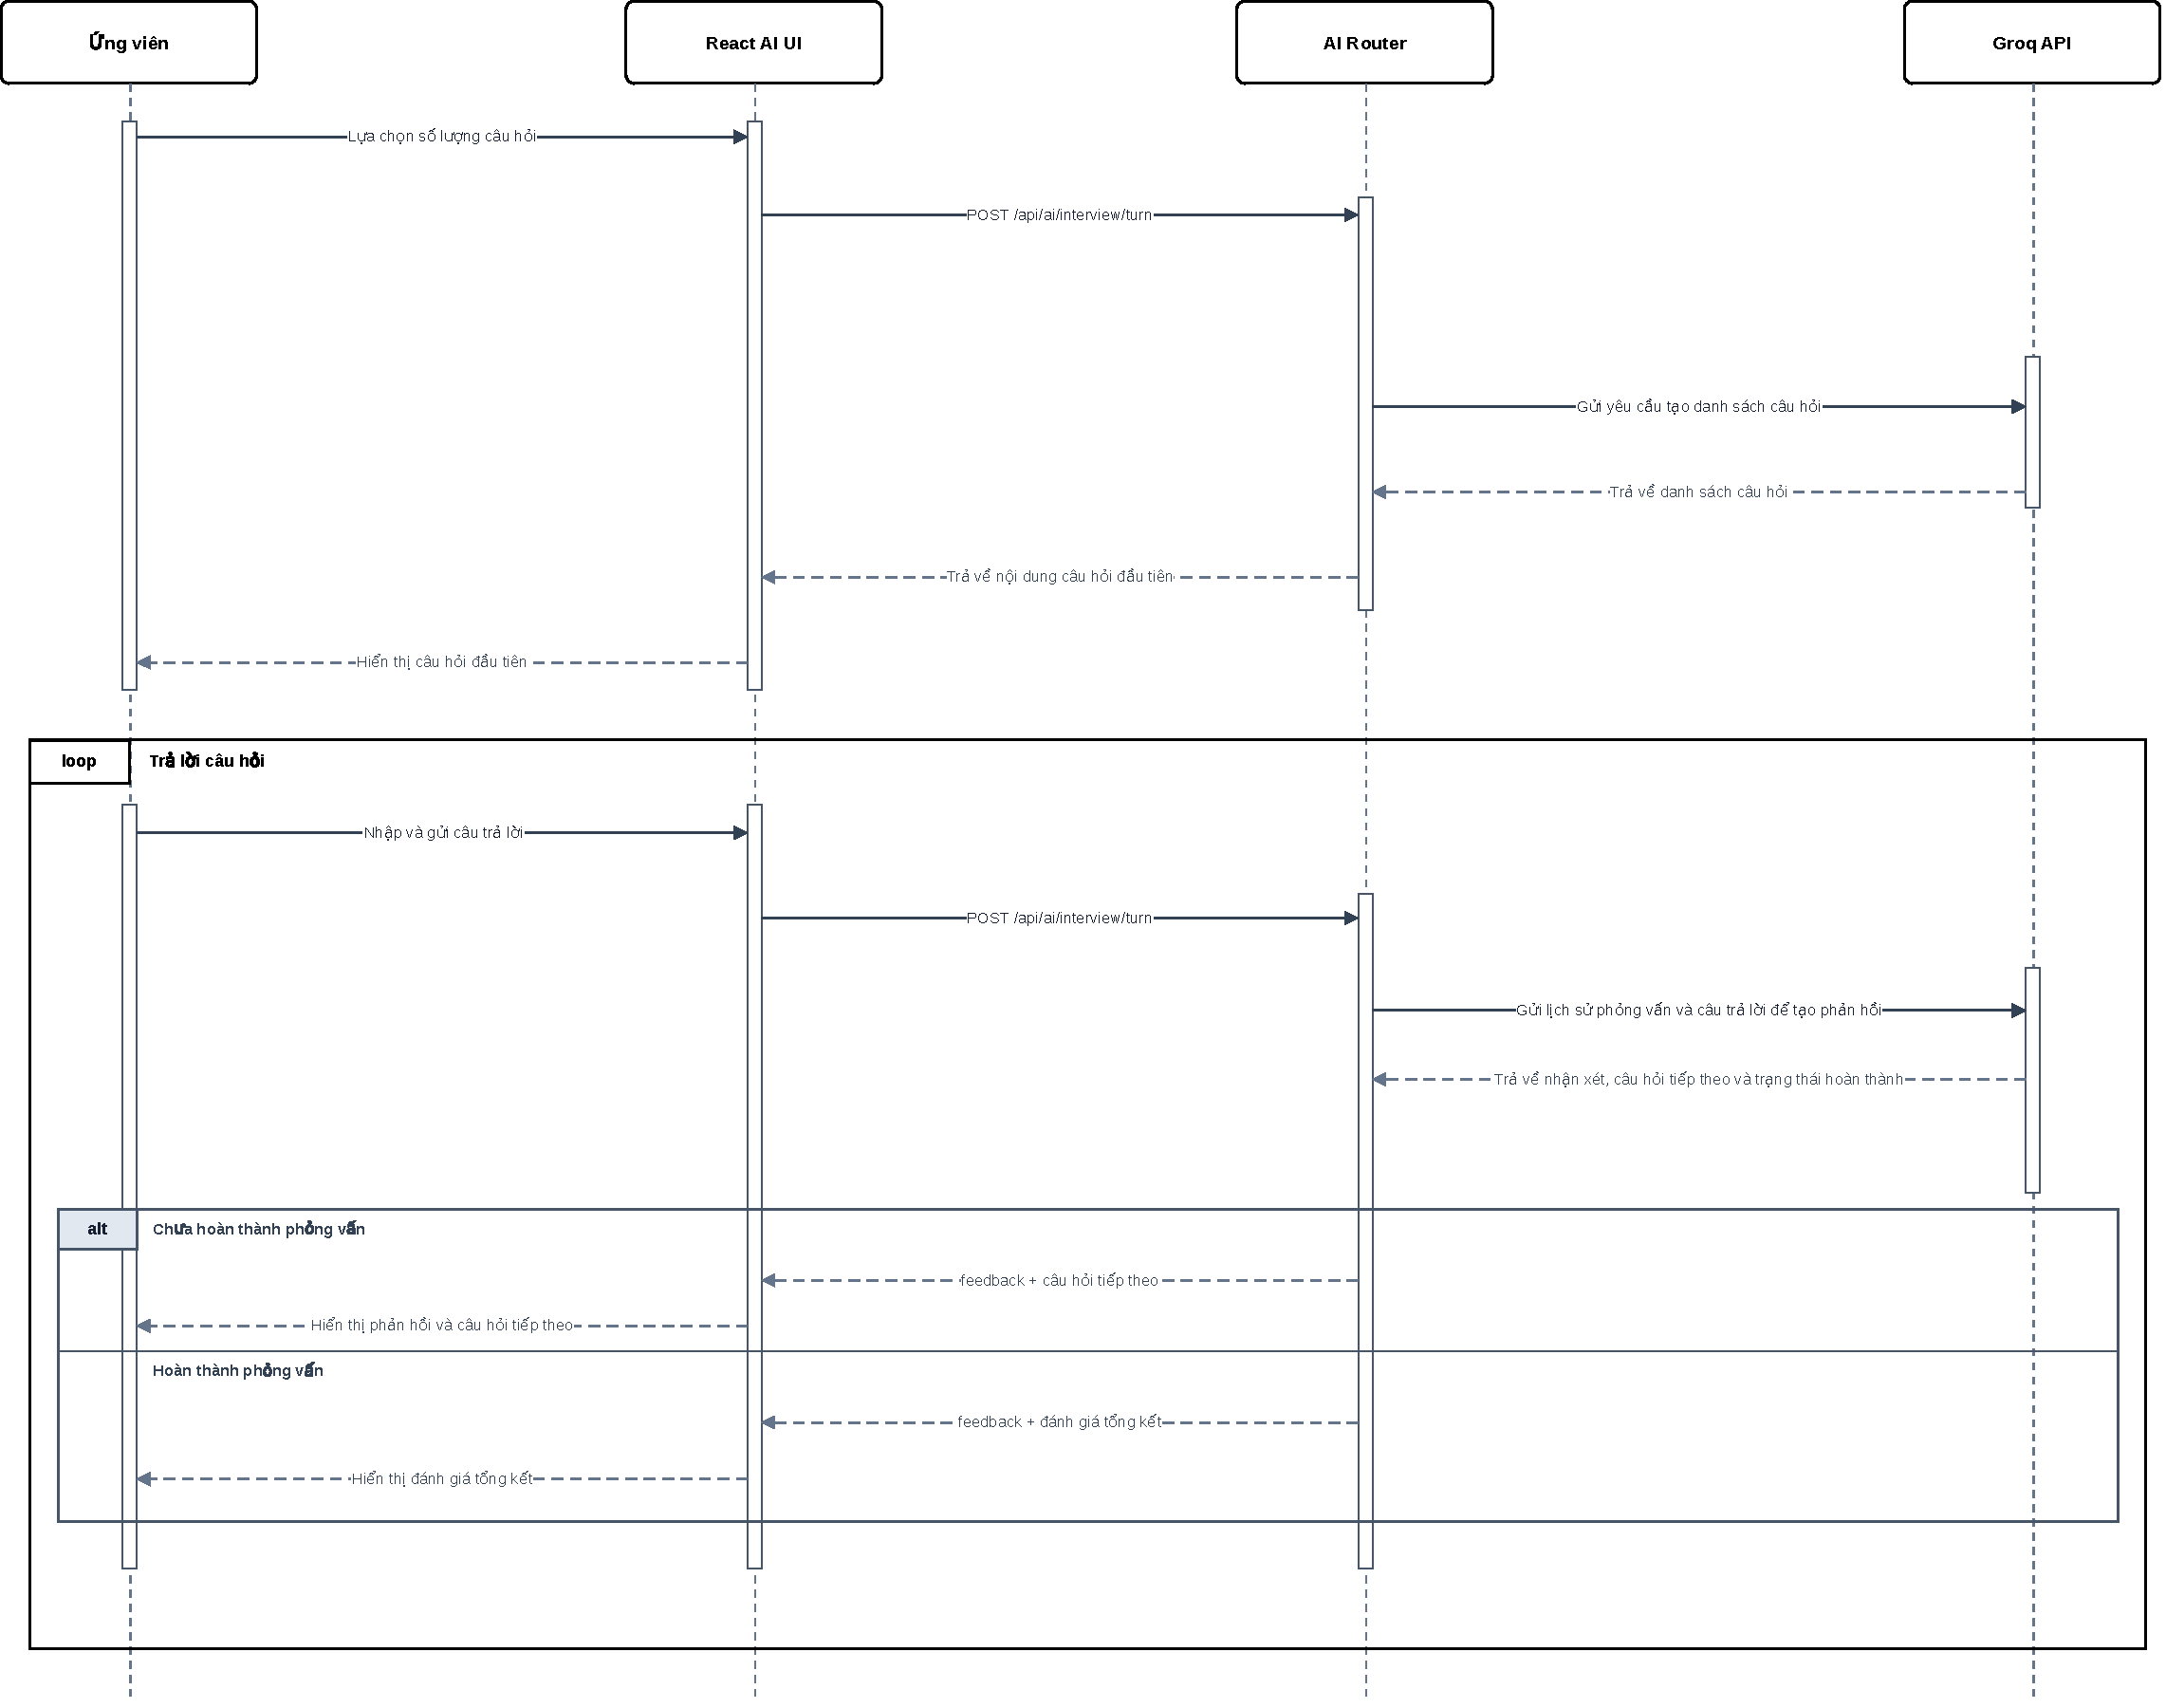
\includegraphics[
            width=1.12\linewidth,
            height=0.68\textheight,
            keepaspectratio
        ]{img/SequenceDiagram_AIInterview.pdf}%
    }
    \caption{Lược đồ tuần tự: Phỏng vấn với AI}
    \label{fig:sequence-diagram-ai-interview}
\end{figure}

Lược đồ tuần tự trong Hình~\ref{fig:sequence-diagram-ai-interview} thể hiện quy trình luyện tập phỏng vấn giữa ứng viên và trợ lý AI:

\begin{itemize}
    \item \textbf{Bắt đầu phỏng vấn:} Ứng viên thiết lập các tiêu chí gồm vị trí ứng tuyển, cấp độ và số lượng câu hỏi. Hệ thống gửi yêu cầu đến dịch vụ AI để tạo bộ câu hỏi phù hợp và hiển thị câu hỏi đầu tiên.
    \item \textbf{Trả lời câu hỏi:} Với mỗi câu hỏi, ứng viên nhập câu trả lời và nhấn gửi. Hệ thống chuyển tiếp nội dung câu trả lời cùng ngữ cảnh phỏng vấn đến AI để chấm điểm, nhận xét và tạo câu hỏi kế tiếp.
    \item \textbf{Kết thúc và đánh giá:} Khi hoàn thành câu hỏi cuối cùng, hệ thống nhận xét tổng thể buổi phỏng vấn và hiển thị bảng đánh giá chi tiết (điểm tổng kết, điểm kỹ năng, gợi ý cải thiện) giúp ứng viên nâng cao năng lực ứng tuyển.
\end{itemize}

\subsection{Ứng tuyển công việc}

\textbf{Ứng tuyển công việc bằng CV đã lưu}
\begin{figure}[H]
    \centering
    \makebox[\linewidth][c]{%
        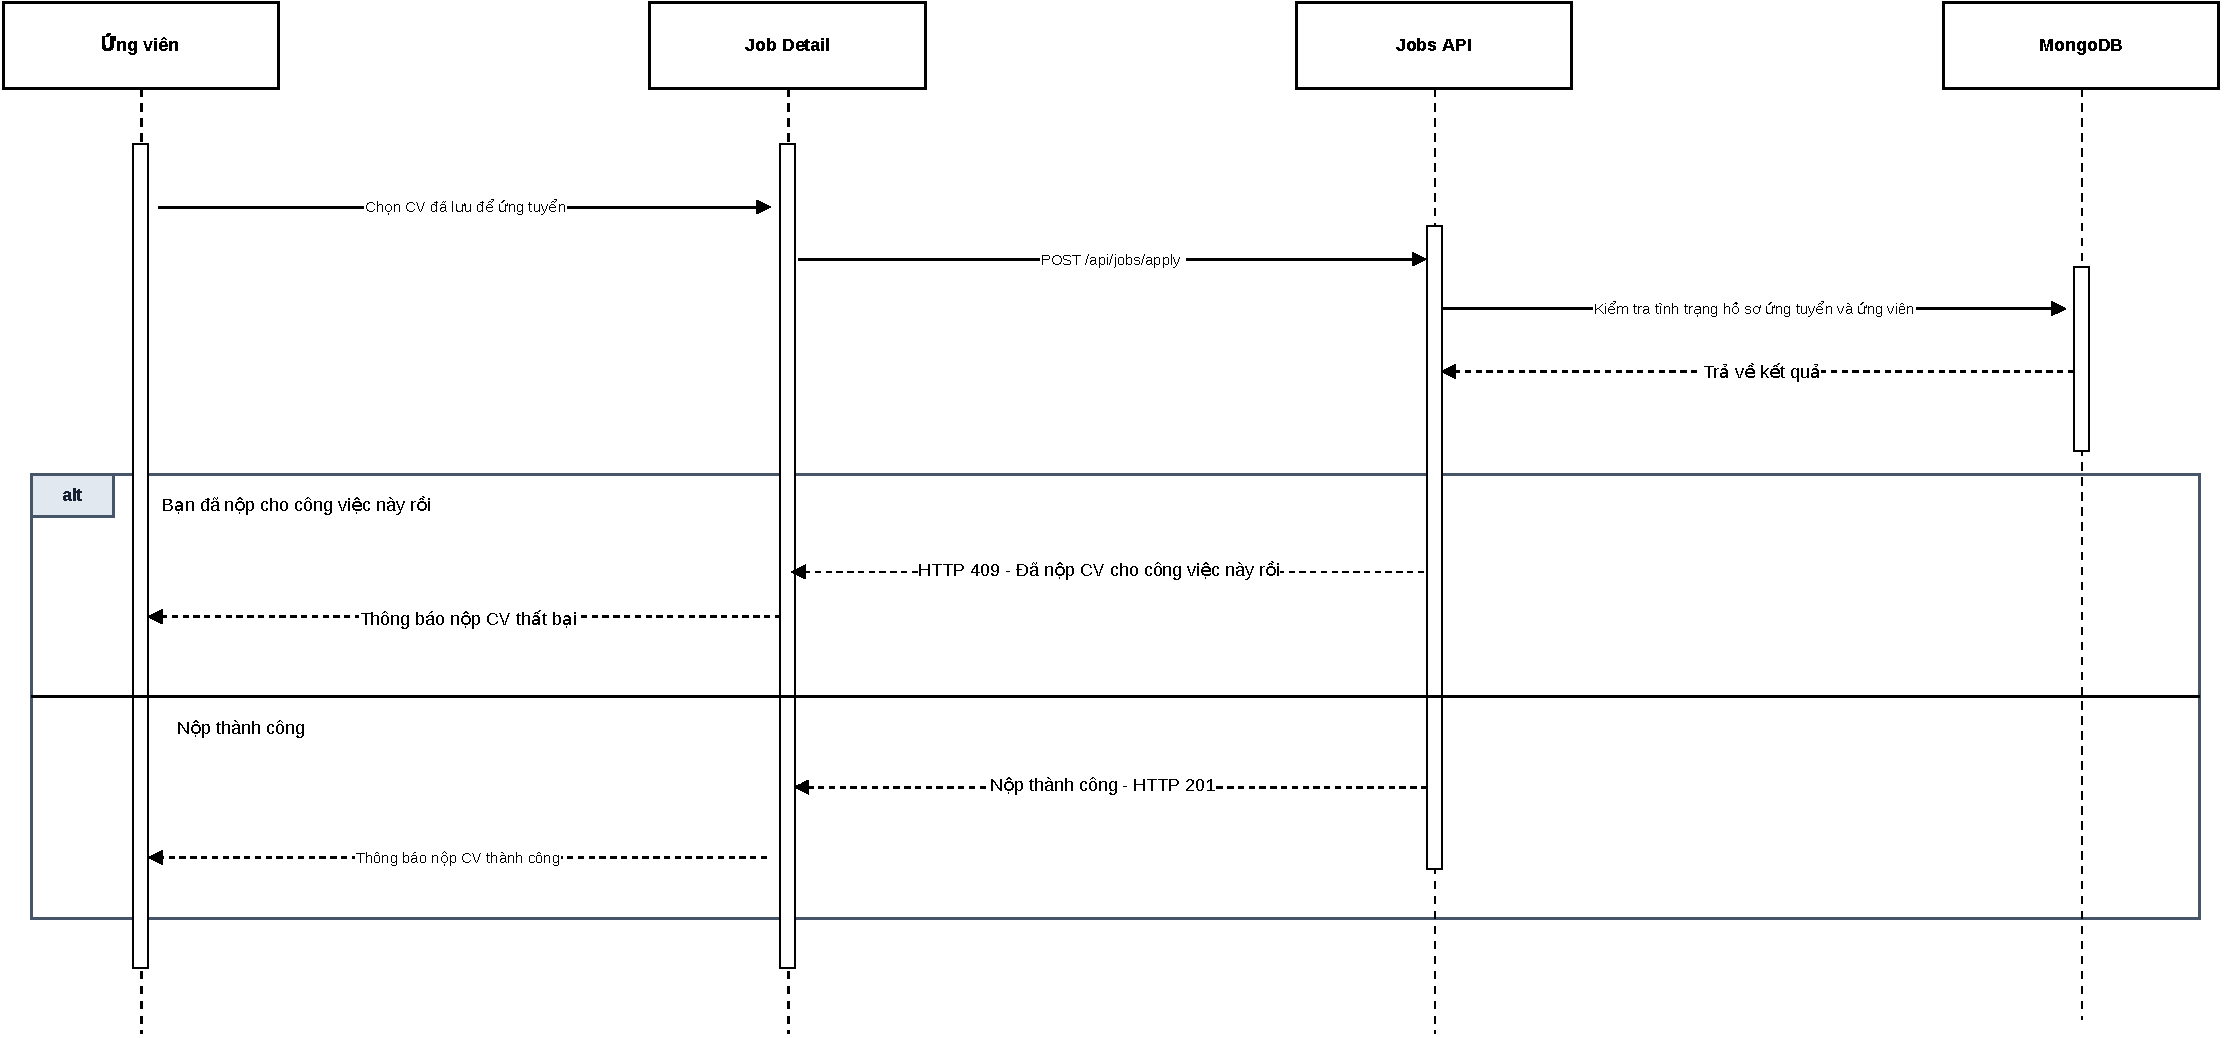
\includegraphics[
            width=1.12\linewidth,
            height=0.60\textheight,
            keepaspectratio
        ]{img/SequenceDiagram_CVApply.pdf}%
    }
    \caption{Lược đồ tuần tự: Ứng tuyển công việc}
    \label{fig:sequence-diagram-cv-apply}
\end{figure}

Lược đồ trong Hình~\ref{fig:sequence-diagram-cv-apply} thể hiện quy trình nộp hồ sơ bằng CV tạo sẵn trên hệ thống. Ứng viên chọn bản CV mong muốn và xác nhận ứng tuyển. Hệ thống kiểm tra trong cơ sở dữ liệu xem ứng viên đã từng nộp hồ sơ vào tin tuyển dụng này chưa. Nếu đã ứng tuyển trước đó, hệ thống từ chối yêu cầu và thông báo trùng lặp. Nếu chưa, hệ thống tạo bản chụp thông tin CV (\texttt{resumeSnapshot}) cùng thông tin việc làm (\texttt{jobSnapshot}), lưu hồ sơ ứng tuyển mới vào cơ sở dữ liệu và thông báo ứng tuyển thành công.

\textbf{Ứng tuyển công việc bằng CV PDF}
\begin{figure}[H]
    \centering
    \makebox[\linewidth][c]{%
        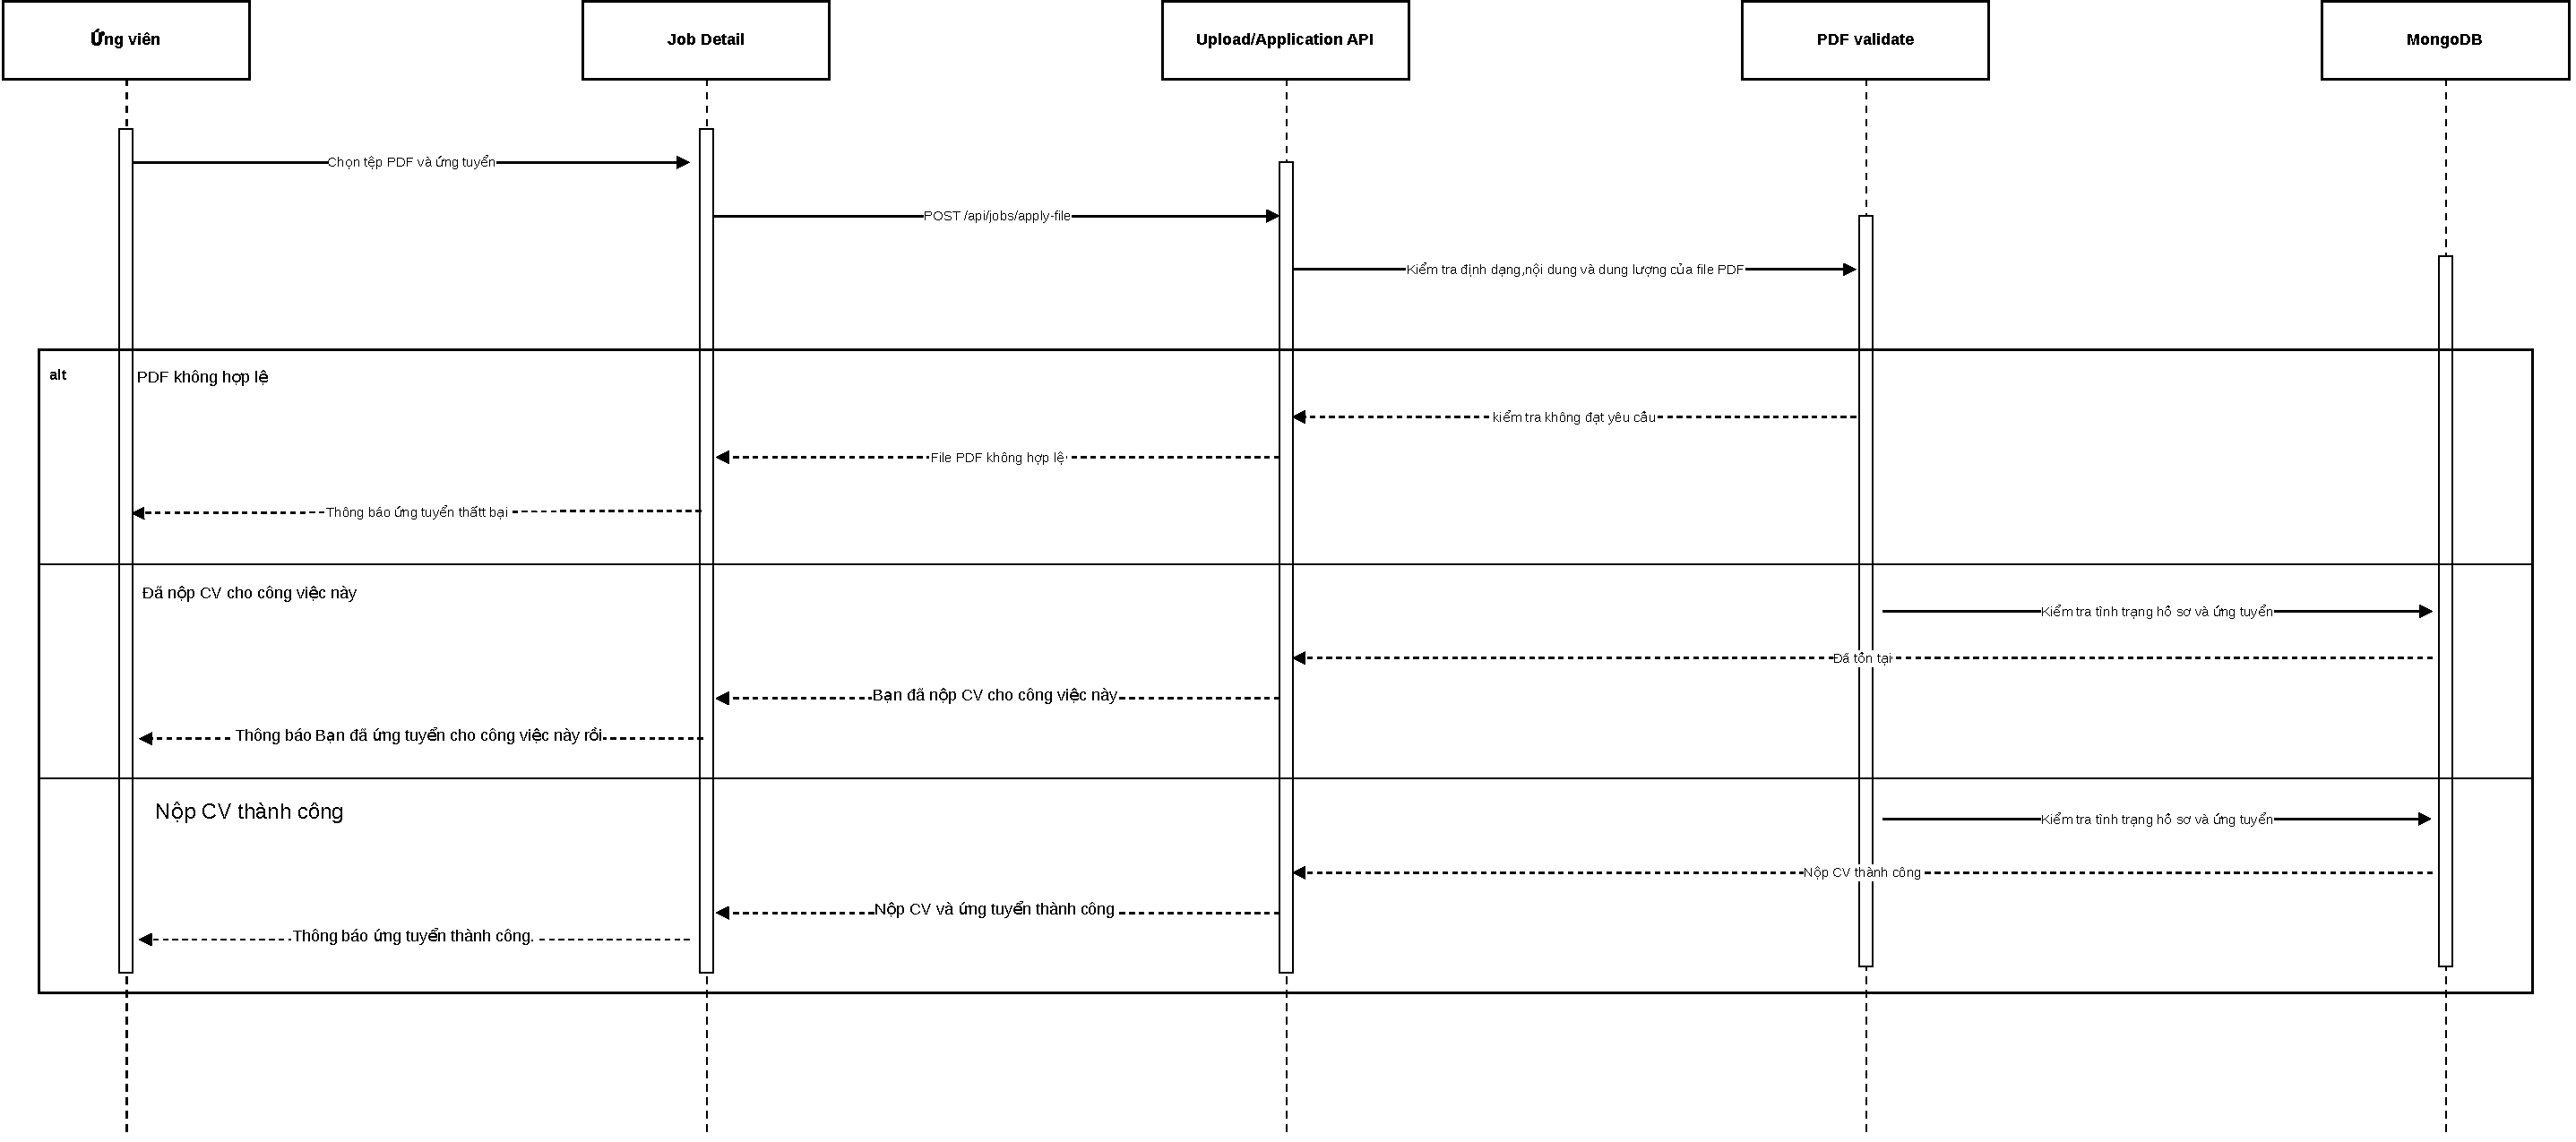
\includegraphics[
            width=1.12\linewidth,
            height=0.60\textheight,
            keepaspectratio
        ]{img/SequenceDiagram_CVPDF.pdf}%
    }
    \caption{Lược đồ tuần tự: Ứng tuyển công việc bằng CV PDF}
    \label{fig:sequence-diagram-cv-pdf}
\end{figure}

Lược đồ trong Hình~\ref{fig:sequence-diagram-cv-pdf} thể hiện quy trình nộp hồ sơ bằng tệp PDF tải lên từ thiết bị. Ứng viên chọn tệp PDF và gửi yêu cầu ứng tuyển. Hệ thống tiến hành kiểm tra định dạng tệp và dung lượng giới hạn (tối đa 5~MB). Nếu tệp không hợp lệ, hệ thống từ chối tiếp nhận và báo lỗi. Nếu tệp hợp lệ, hệ thống kiểm tra trạng thái trùng lặp hồ sơ; sau khi xác nhận chưa nộp, hệ thống lưu trữ tệp, ghi nhận hồ sơ ứng tuyển vào cơ sở dữ liệu và gửi thông báo thành công cho ứng viên.

\subsection{Quản lý tin tuyển dụng}

\begin{figure}[H]
    \centering
    \makebox[\linewidth][c]{%
        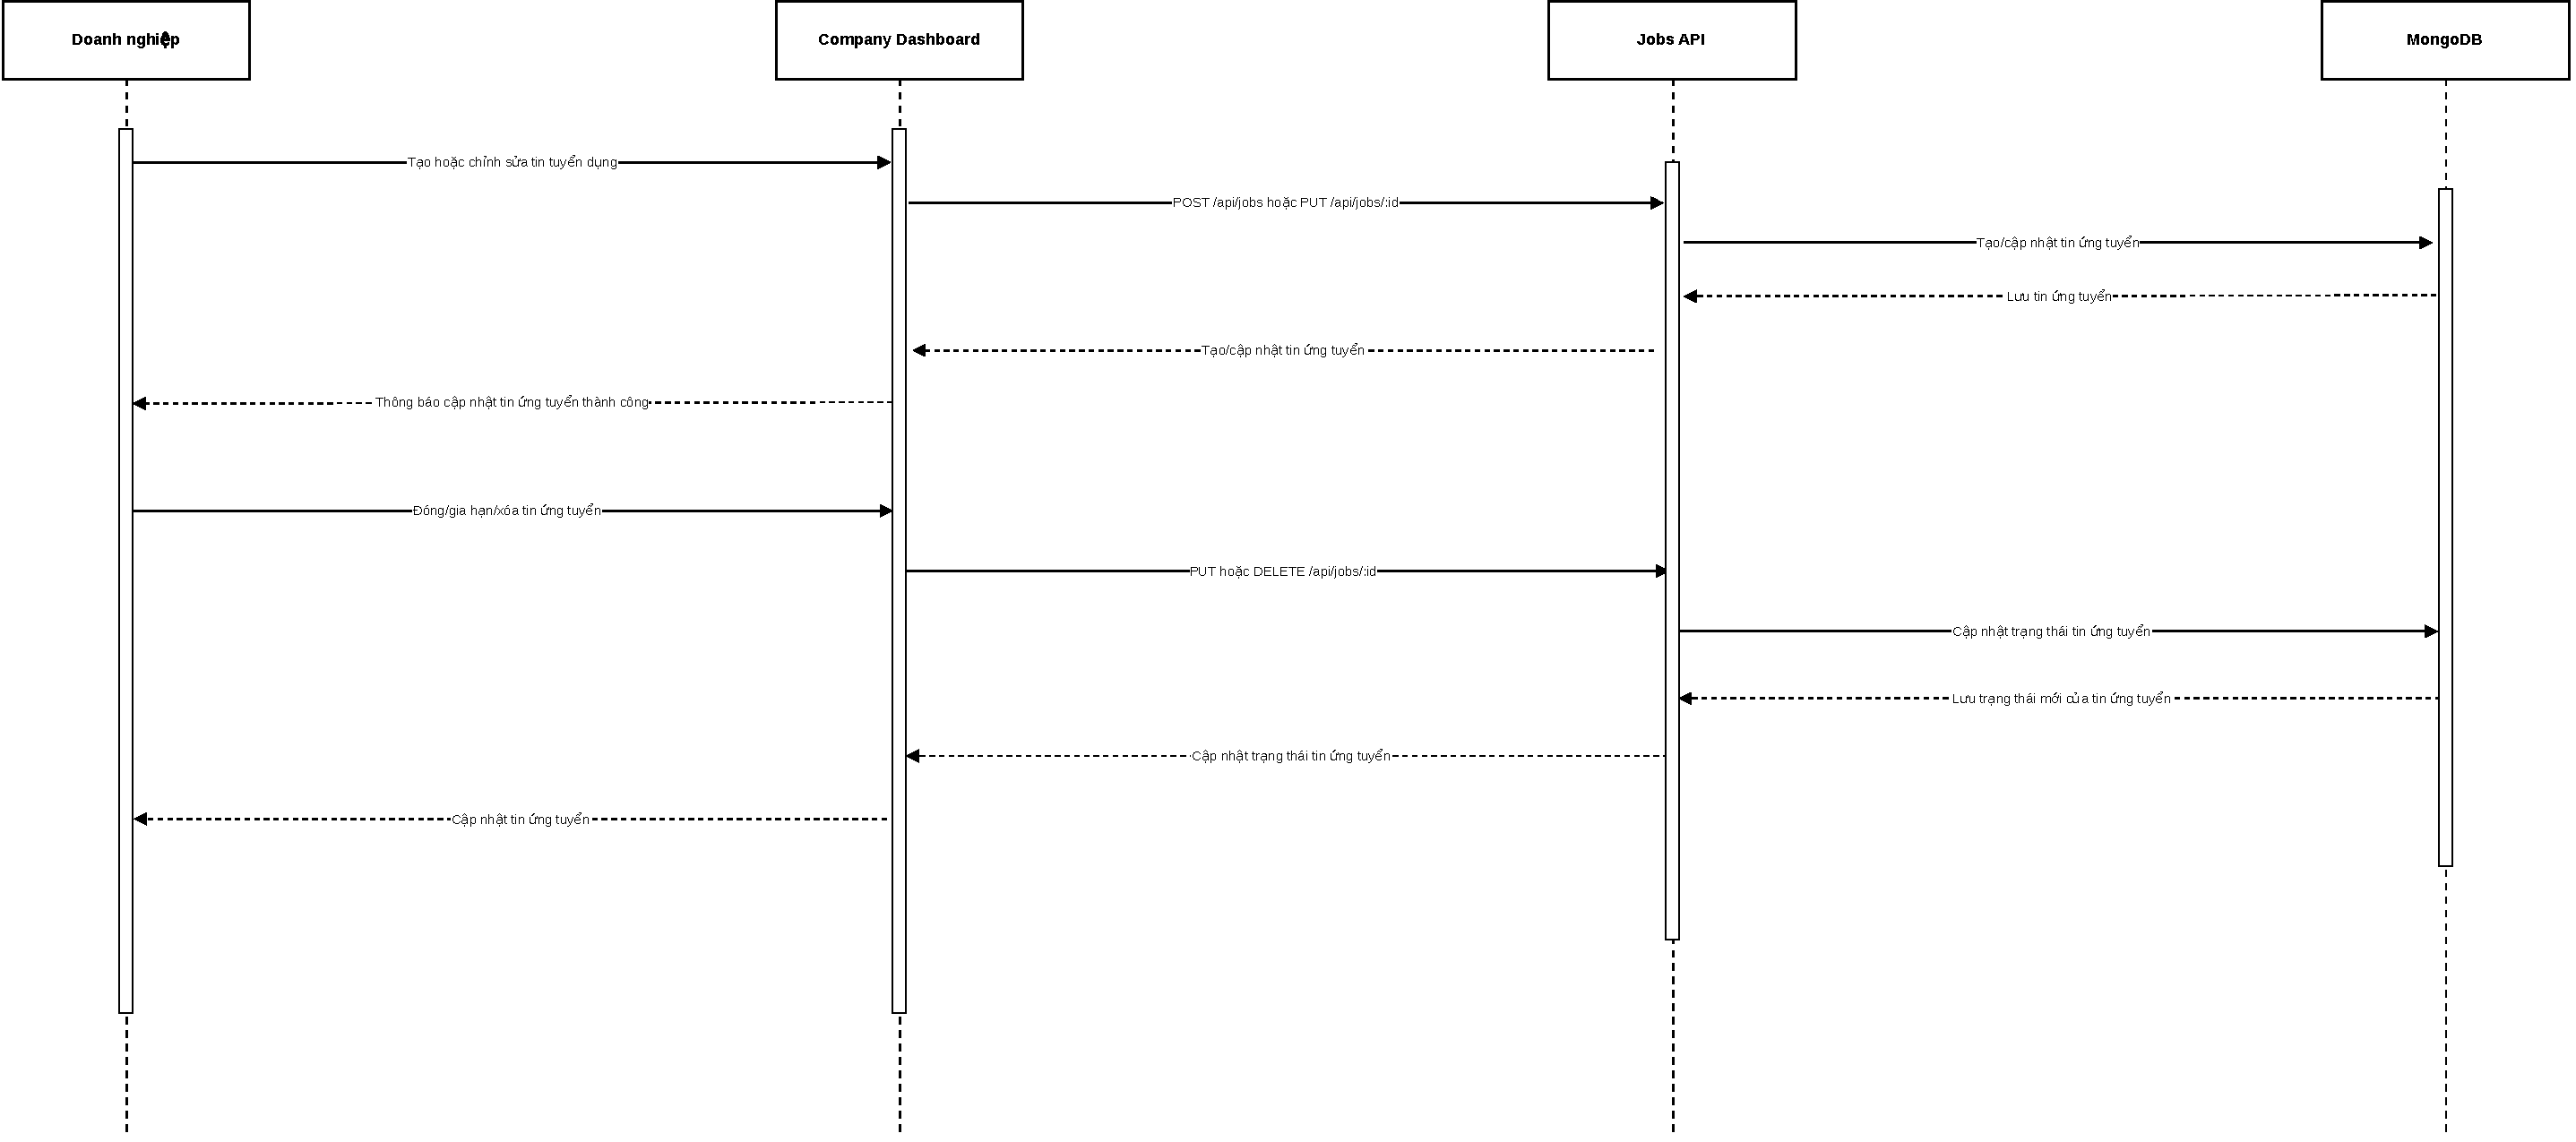
\includegraphics[
            width=1.12\linewidth,
            height=0.60\textheight,
            keepaspectratio
        ]{img/SequenceDiagram_JobsManagement.pdf}%
    }
    \caption{Lược đồ tuần tự: Quản lý tin tuyển dụng}
    \label{fig:sequence-diagram-jobs-management}
\end{figure}

Lược đồ tuần tự trong Hình~\ref{fig:sequence-diagram-jobs-management} thể hiện quy trình quản lý tin tuyển dụng của doanh nghiệp:

\begin{itemize}
    \item \textbf{Tạo hoặc chỉnh sửa tin tuyển dụng:} Doanh nghiệp nhập thông tin bài đăng mới hoặc cập nhật nội dung tin đã có. Hệ thống tiếp nhận, xác thực dữ liệu và lưu vào cơ sở dữ liệu, sau đó phản hồi thông báo hoàn tất cho doanh nghiệp.
    \item \textbf{Đóng, gia hạn hoặc xóa tin tuyển dụng:} Doanh nghiệp có thể chủ động đóng tin khi đã tuyển đủ số lượng, gia hạn thời gian nhận hồ sơ hoặc xóa bài đăng. Hệ thống cập nhật trạng thái mới hoặc xóa bản ghi tương ứng trong cơ sở dữ liệu và làm mới danh sách quản lý.
\end{itemize}

\subsection{Chat và thông báo}

\medskip
\textbf{Nhắn tin theo thời gian thực}
\medskip
\begin{figure}[H]
    \centering
    \makebox[\linewidth][c]{%
        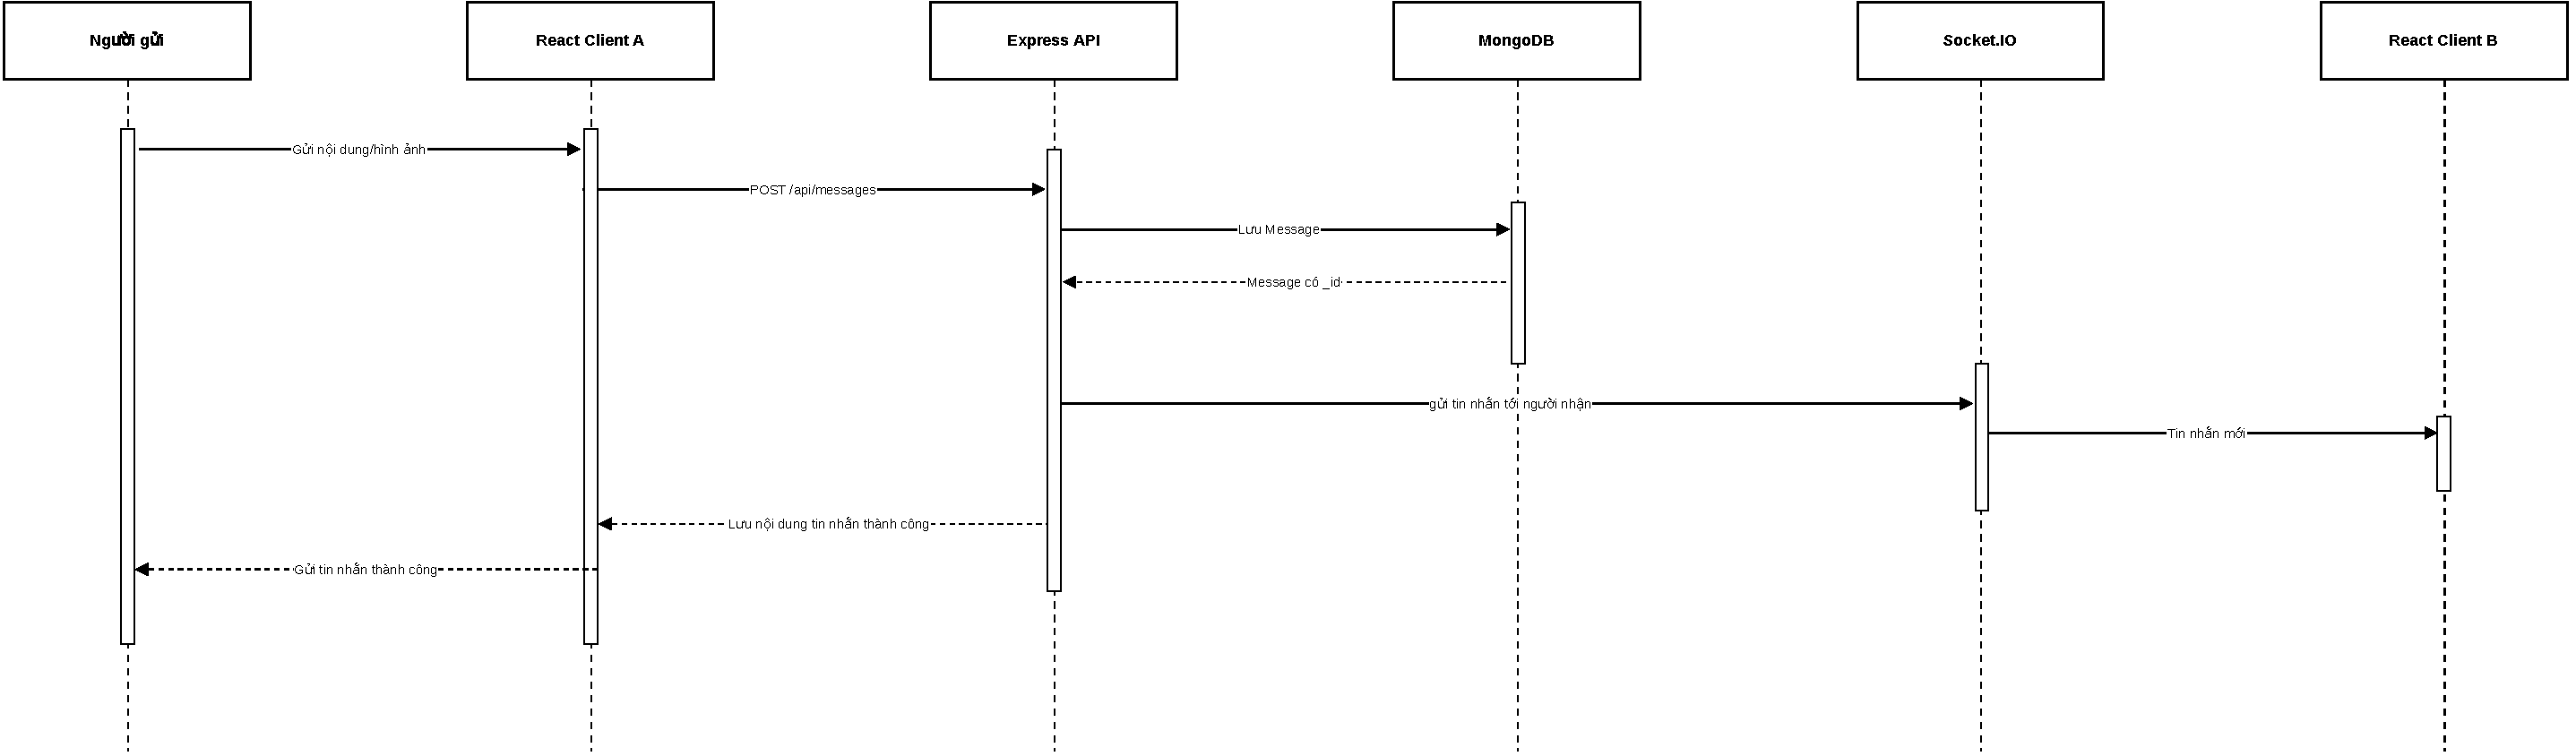
\includegraphics[
            width=1.12\linewidth,
            height=0.68\textheight,
            keepaspectratio
        ]{img/SequenceDiagram_Chat.pdf}%
    }
    \caption{Lược đồ tuần tự: Nhắn tin theo thời gian thực}
    \label{fig:sequence-diagram-chat}
\end{figure}

Lược đồ tuần tự trong Hình~\ref{fig:sequence-diagram-chat} thể hiện quy trình nhắn tin trao đổi trực tiếp giữa ứng viên và doanh nghiệp theo thời gian thực:

\begin{itemize}
    \item \textbf{Gửi tin nhắn:} Người dùng nhập nội dung văn bản hoặc đính kèm hình ảnh và nhấn gửi. Hệ thống kiểm tra tính hợp lệ của nội dung tin nhắn trước khi xử lý.
    \item \textbf{Lưu trữ và chuyển tiếp:} Hệ thống lưu bản ghi tin nhắn mới vào cơ sở dữ liệu MongoDB, đồng thời sử dụng kết nối Socket.IO để chuyển tiếp tức thì tin nhắn đến người nhận trong phòng chat. Hệ thống phản hồi xác nhận cho người gửi và đồng bộ nội dung mới lên giao diện của cả hai phía.
\end{itemize}

\medskip
\textbf{Thông báo}
\medskip
\begin{figure}[H]
    \centering
    \makebox[\linewidth][c]{%
        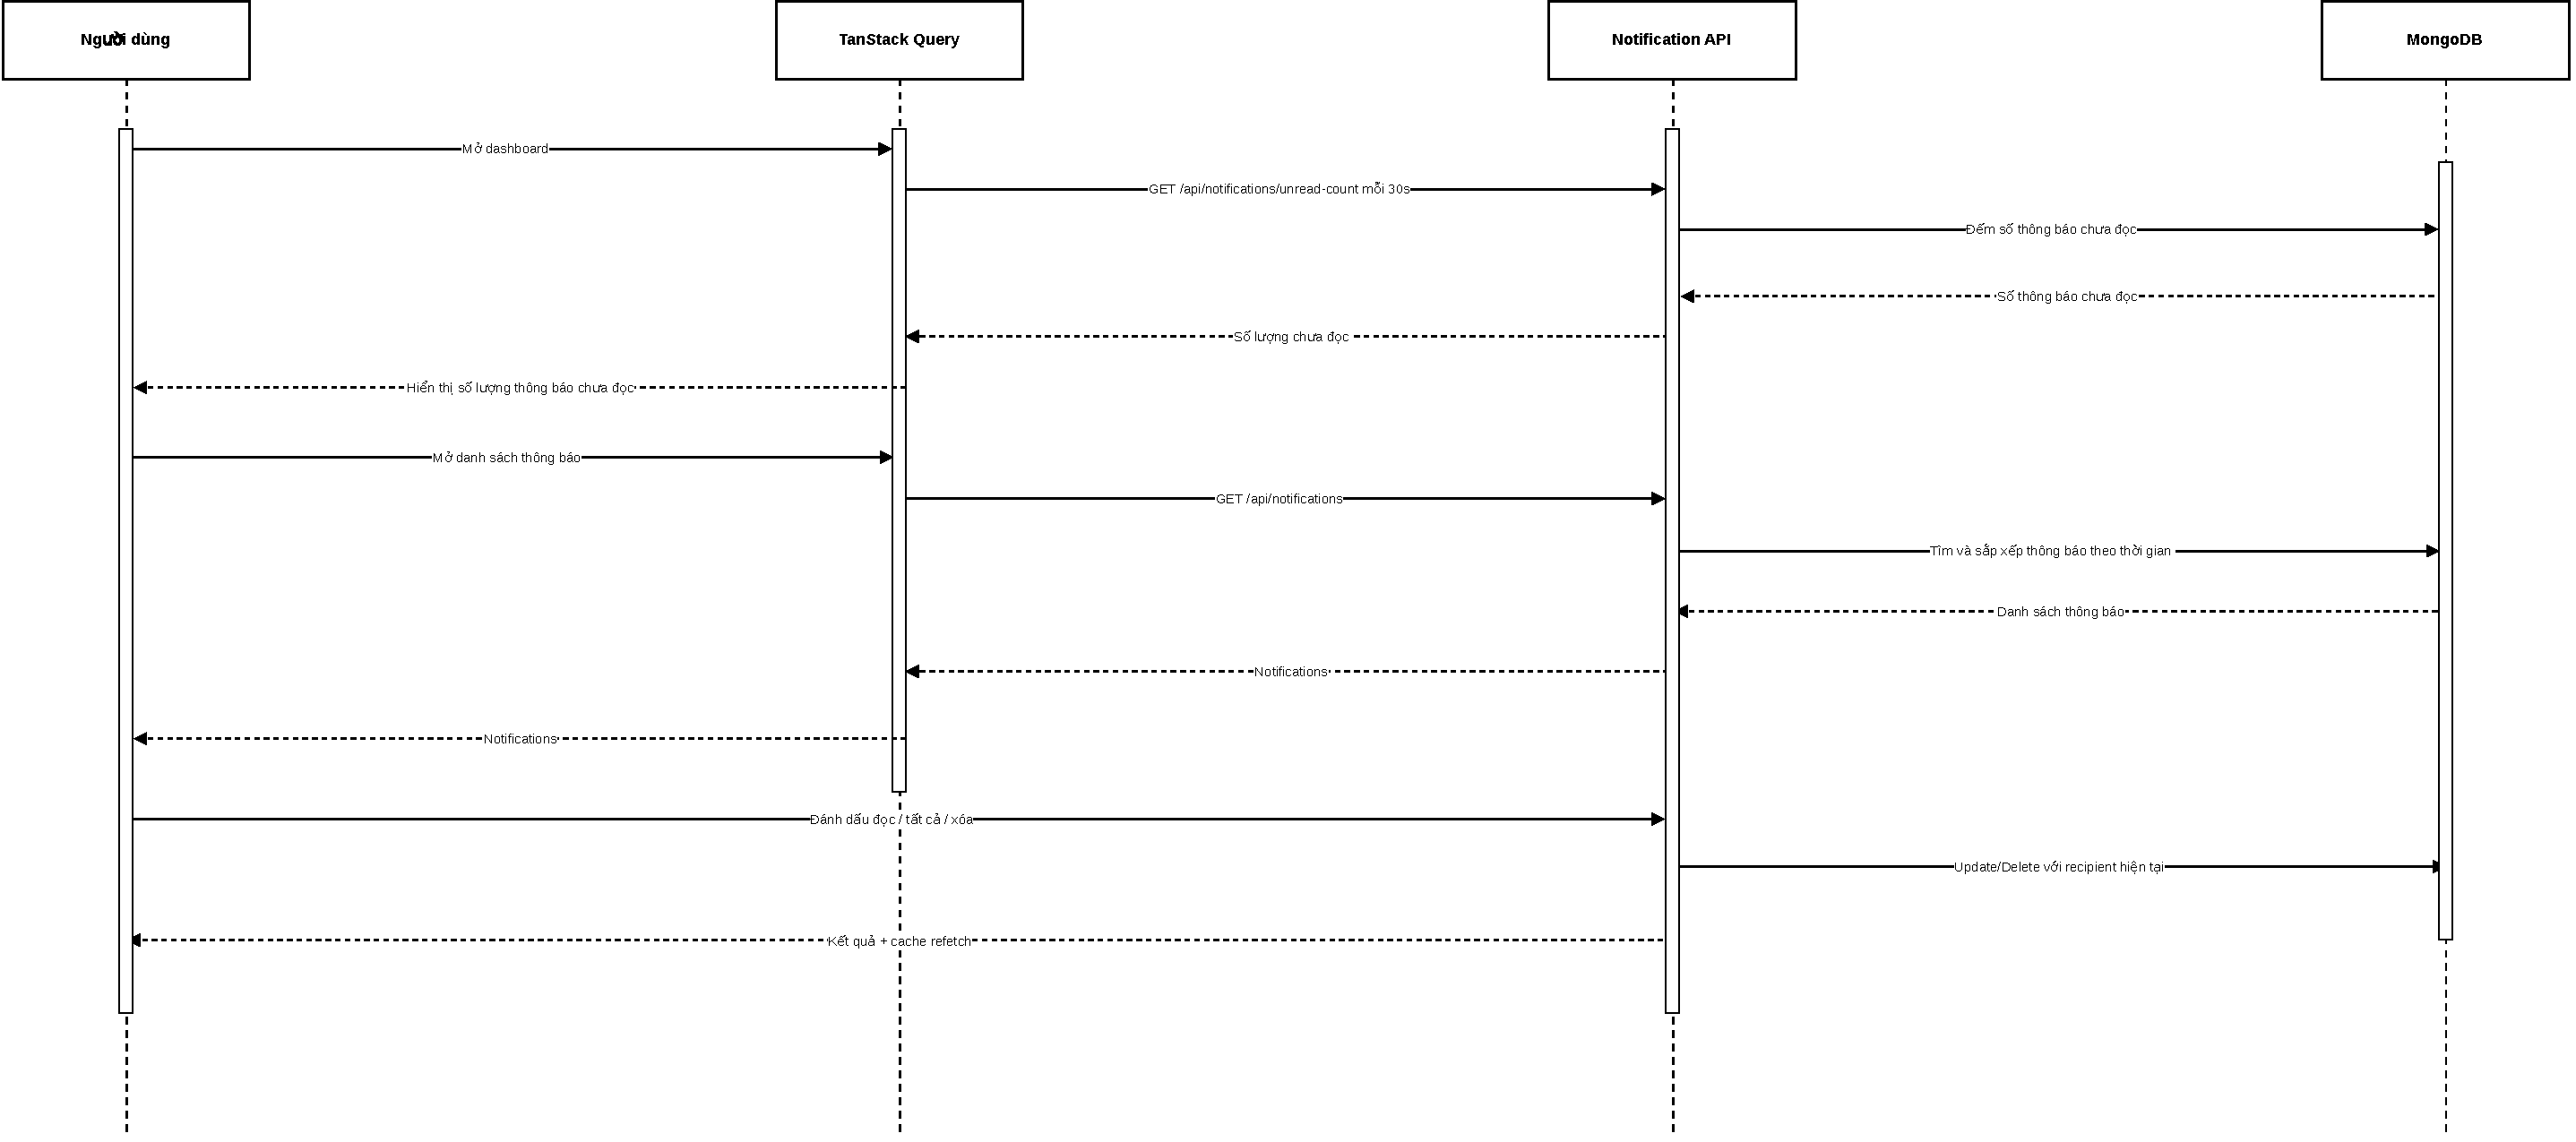
\includegraphics[
            width=1.12\linewidth,
            height=0.68\textheight,
            keepaspectratio
        ]{img/SequenceDiagram_Notification.pdf}%
    }
    \caption{Lược đồ tuần tự: Thông báo}
    \label{fig:sequence-diagram-notification}
\end{figure}

Lược đồ tuần tự trong Hình~\ref{fig:sequence-diagram-notification} thể hiện quy trình hiển thị, quản lý và xử lý thông báo của người dùng:

\begin{itemize}
    \item \textbf{Kiểm tra thông báo chưa đọc:} Khi người dùng mở ứng dụng, hệ thống tự động kiểm tra định kỳ mỗi 30 giây để cập nhật số lượng thông báo mới chưa đọc lên biểu tượng chuông thông báo.
    \item \textbf{Xem danh sách thông báo:} Khi người dùng bấm vào biểu tượng chuông, hệ thống truy vấn cơ sở dữ liệu để lấy danh sách thông báo, sắp xếp theo thời gian mới nhất (giảm dần) và hiển thị chi tiết cho người dùng.
    \item \textbf{Cập nhật trạng thái thông báo:} Khi người dùng nhấn xem một thông báo cụ thể hoặc chọn đánh dấu tất cả đã đọc, hệ thống gửi yêu cầu cập nhật trạng thái trong cơ sở dữ liệu và làm mới giao diện hiển thị.
\end{itemize}

\subsection{Quản trị viên}
\begin{figure}[H]
    \centering
    \makebox[\linewidth][c]{%
        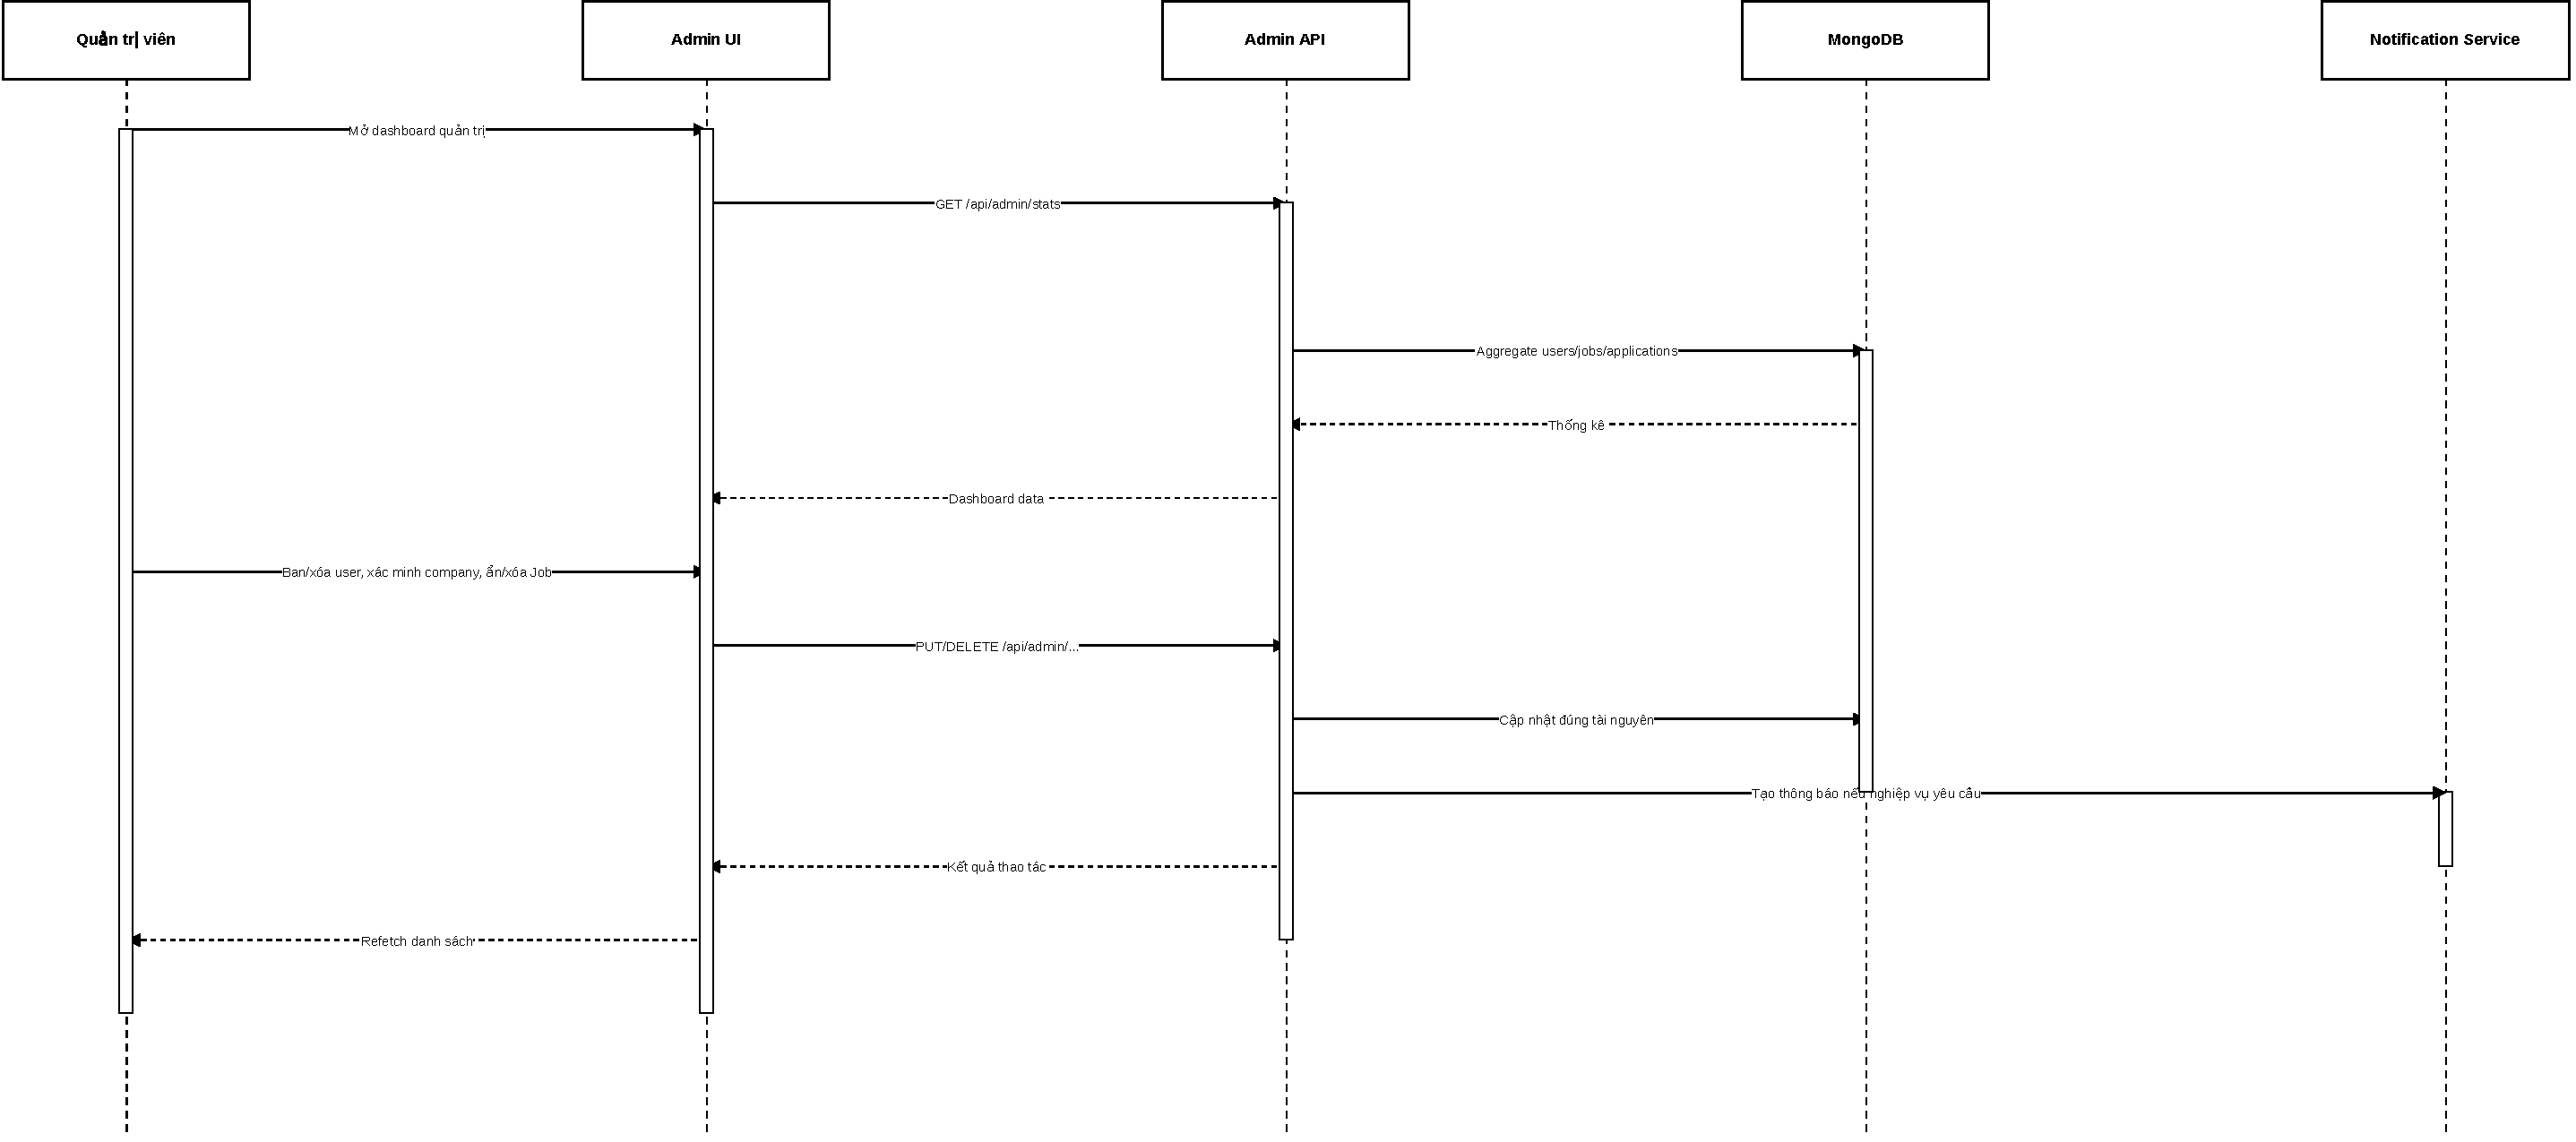
\includegraphics[
            width=1.12\linewidth,
            height=0.68\textheight,
            keepaspectratio
        ]{img/SequenceDiagram_Admin.pdf}%
    }
    \caption{Lược đồ tuần tự: Quản trị viên}
    \label{fig:sequence-diagram-admin}
\end{figure}

Lược đồ tuần tự trong Hình~\ref{fig:sequence-diagram-admin} thể hiện các quy trình thực hiện công việc của quản trị viên:

\begin{itemize}
    \item \textbf{Xem thống kê hệ thống:} Khi quản trị viên truy cập bảng điều khiển, hệ thống tự động tổng hợp số liệu từ cơ sở dữ liệu về người dùng, doanh nghiệp, tin tuyển dụng và hồ sơ ứng tuyển để trực quan hóa qua biểu đồ thống kê.
    \item \textbf{Quản lý người dùng và doanh nghiệp:} Quản trị viên tra cứu danh sách để thực hiện các thao tác như khóa hoặc mở khóa tài khoản vi phạm, xác minh hoặc từ chối thông tin đăng ký doanh nghiệp. Hệ thống cập nhật trạng thái tương ứng vào cơ sở dữ liệu.
    \item \textbf{Kiểm duyệt tin tuyển dụng:} Quản trị viên kiểm tra các bài đăng việc làm trên hệ thống, có quyền ẩn bài đăng vi phạm hoặc xóa tin tuyển dụng để bảo vệ quyền lợi ứng viên.
\end{itemize}

\clearpage
\section{Lược đồ lớp (Class Diagram)}

Lược đồ lớp trong Hình~\ref{fig:class-diagram-overview} thể hiện cấu trúc hướng đối tượng và mối quan hệ giữa các thành phần trong hệ thống RabbitCV. Hệ thống được tổ chức theo mô hình kiến trúc phân tầng (Layered Architecture) với ba tầng chính: Controller, Service và Model:

\begin{itemize}
    \item \textbf{Tầng Controller:} Tiếp nhận các yêu cầu HTTP từ phía client, kiểm tra tính hợp lệ của dữ liệu và điều phối xử lý đến tầng Service tương ứng. Các lớp điều khiển chính bao gồm:
    \begin{itemize}
        \item \texttt{AuthController}, \texttt{UserController}: Xử lý xác thực, phân quyền và quản lý tài khoản người dùng.
        \item \texttt{ResumeController}, \texttt{JobController}: Quản lý tạo mới, chỉnh sửa CV và tin tuyển dụng.
        \item \texttt{ApplicationController}: Xử lý nộp hồ sơ ứng tuyển và quản lý trạng thái hồ sơ.
        \item \texttt{ChatController}, \texttt{NotificationController}: Điều phối tin nhắn thời gian thực và thông báo.
        \item \texttt{AdminController}, \texttt{AIController}: Quản trị hệ thống và điều phối các tác vụ AI thông minh.
    \end{itemize}
    \item \textbf{Tầng Service:} Hiện thực hóa toàn bộ logic nghiệp vụ, quản lý luồng dữ liệu và tích hợp các dịch vụ bên ngoài:
    \begin{itemize}
        \item Các service cơ sở (\texttt{AuthService}, \texttt{UserService}, \texttt{ResumeService}, \texttt{JobService}, \texttt{ApplicationService}, \texttt{AdminService}) đảm bảo tính toàn vẹn dữ liệu, xác thực phân quyền và thực hiện các quy trình nghiệp vụ trọng yếu.
        \item \texttt{ChatService} tích hợp với \texttt{RealtimeGateway} (sử dụng thư viện Socket.IO) nhằm quản lý kết nối WebSocket thời gian thực, duy trì trạng thái kết nối phòng chat và chuyển tiếp tin nhắn tức thì giữa ứng viên và nhà tuyển dụng.
        \item \texttt{AIService} chịu trách nhiệm giao tiếp với dịch vụ AI thông qua Groq API; phương thức \texttt{checkUserDailyLimit} thực hiện kiểm tra hạn mức sử dụng hằng ngày của người dùng và dữ liệu phản hồi được chuẩn hóa theo JSON Schema.
    \end{itemize}
    \item \textbf{Tầng Model:} Định nghĩa cấu trúc dữ liệu và các mối quan hệ thực thể được quản lý trong cơ sở dữ liệu MongoDB, bao gồm các lớp: \texttt{User}, \texttt{Resume} (kèm \texttt{PersonalInfo}), \texttt{Job}, \texttt{Application}, \texttt{Message}, \texttt{Notification}, \texttt{AiUsage} và \texttt{SavedJob}. Các mối quan hệ sở hữu, ứng tuyển, gửi tin nhắn và lưu tin được thiết lập chặt chẽ nhằm đảm bảo tính nhất quán của dữ liệu.
\end{itemize}

\clearpage

\begin{figure}[htbp]
    \centering
    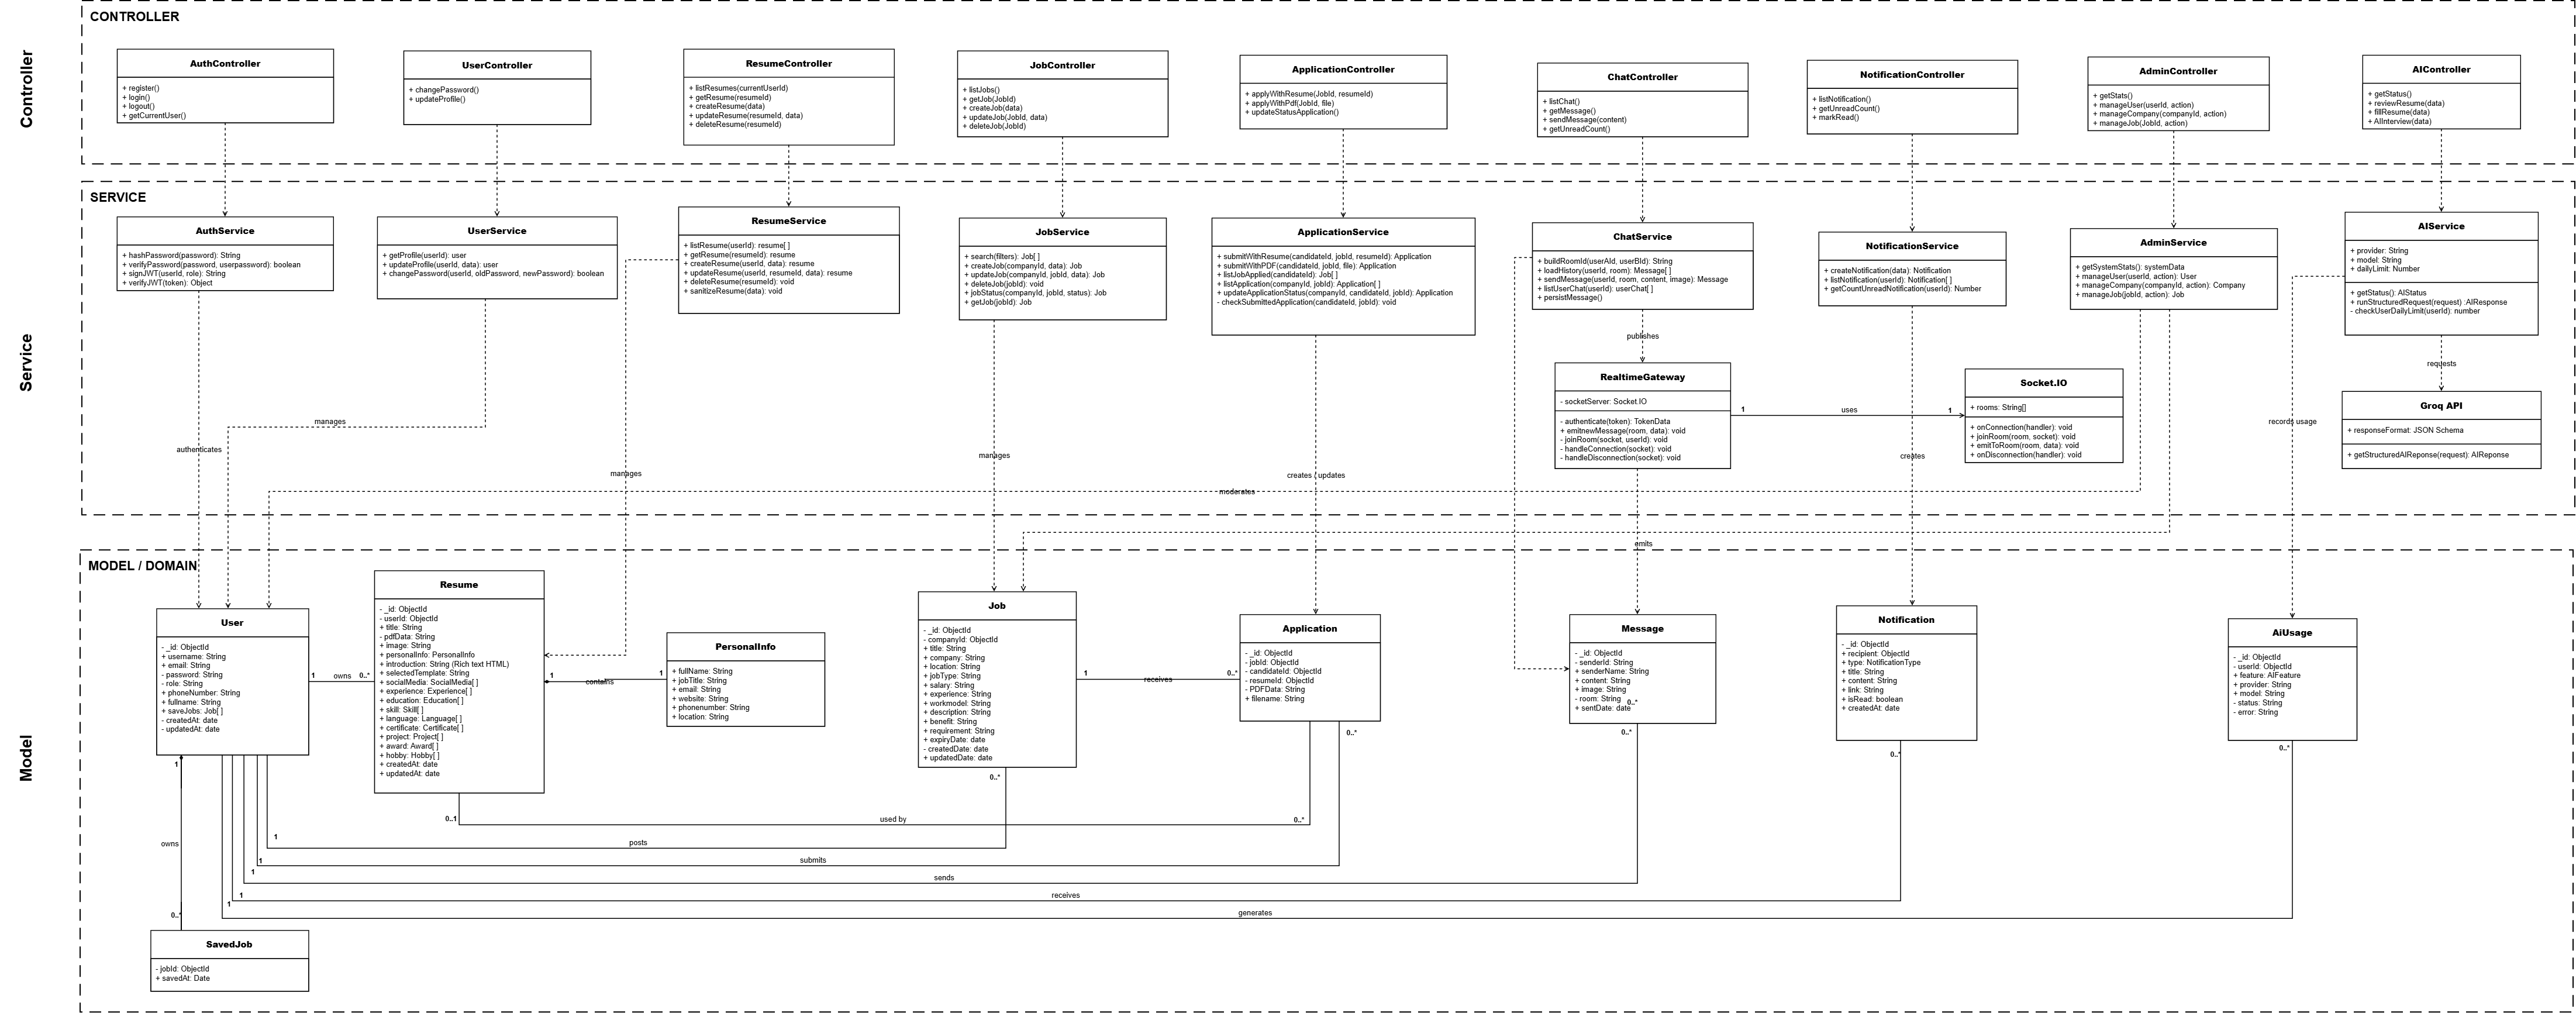
\includegraphics[
        angle=90,
        width=1\linewidth,
        height=0.90\textheight,
        keepaspectratio
    ]{img/classDiagram_overview.png}
    \caption{Lược đồ lớp tổng quan hệ thống RabbitCV}
    \label{fig:class-diagram-overview}
\end{figure}

\clearpage

\section{Lược đồ kiến trúc hệ thống (Architecture Diagram)}

Lược đồ kiến trúc trong Hình~\ref{fig:architecture-diagram} mô tả cấu trúc phân tầng tổng thể, các khối thành phần chức năng, phương thức giao tiếp và luồng dữ liệu của hệ thống RabbitCV từ thiết bị người dùng đến máy chủ, cơ sở dữ liệu và các dịch vụ ngoại vi.

\begin{figure}[H]
    \centering
    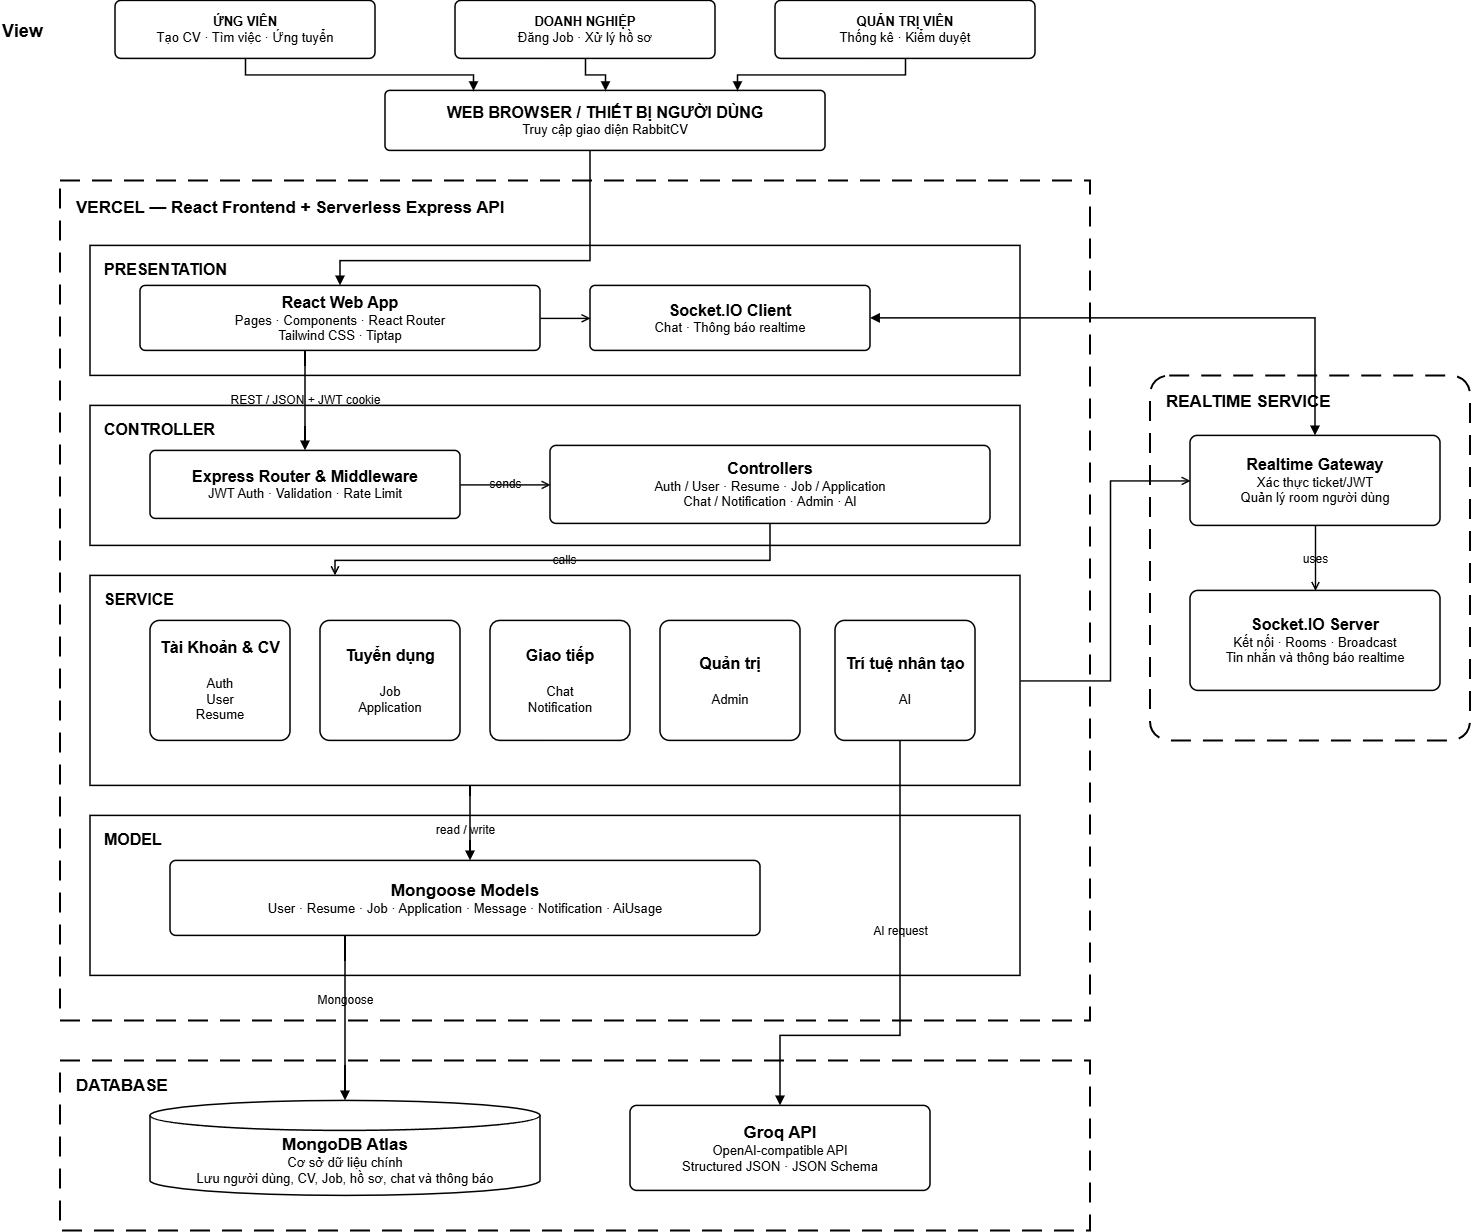
\includegraphics[
        width=0.95\linewidth,
        height=0.82\textheight,
        keepaspectratio
    ]{img/architecture_diagram.png}
    \caption{Lược đồ kiến trúc tổng thể hệ thống RabbitCV}
    \label{fig:architecture-diagram}
\end{figure}

Hệ thống được tổ chức thành các phân vùng và tầng kiến trúc chính như sau:

\begin{enumerate}
    \item \textbf{Tầng tác nhân và điểm truy cập người dùng (User \& Client Layer):}
    \begin{itemize}
        \item \textbf{Các nhóm tác nhân chính:} Bao gồm ba nhóm người dùng có vai trò khác nhau trong hệ sinh thái:
        \begin{itemize}
            \item \textit{Ứng viên (Candidate):} Thao tác tạo, chỉnh sửa CV, tìm kiếm việc làm và nộp hồ sơ ứng tuyển trực tuyến.
            \item \textit{Doanh nghiệp (Company):} Thực hiện đăng tin tuyển dụng việc làm, tiếp nhận và quản lý quy trình xét duyệt hồ sơ ứng viên.
            \item \textit{Quản trị viên (Administrator):} Theo dõi số liệu thống kê hệ thống, kiểm duyệt nội dung tin tuyển dụng và quản lý tài khoản người dùng.
        \end{itemize}
        \item \textbf{Trình duyệt web và thiết bị người dùng:} Người dùng sử dụng các thiết bị đầu cuối (máy tính, máy tính bảng, điện thoại di động) để truy cập ứng dụng thông qua trình duyệt web hỗ trợ các chuẩn web hiện đại.
    \end{itemize}

    \item \textbf{Khối ứng dụng chính:}
    Nền tảng ứng dụng được triển khai theo mô hình đám mây trên hạ tầng Vercel, chia thành các tầng xử lý có trách nhiệm rõ ràng:
    \begin{itemize}
        \item \textbf{Tầng trình diễn (Presentation Layer):}
        \begin{itemize}
            \item \textit{React Web App:} Xây dựng ứng dụng trang đơn (Single-Page Application -- SPA) với các component giao diện trực quan, quản lý luồng điều hướng trang thông qua React Router, tạo phong cách giao diện với Tailwind CSS và tích hợp trình soạn thảo nội dung chuyên sâu Tiptap.
            \item \textit{Socket.IO Client:} Thành phần client chịu trách nhiệm thiết lập và duy trì kết nối WebSocket hai chiều đến dịch vụ Realtime Gateway để trao đổi tin nhắn trò chuyện (Chat) và cập nhật thông báo tức thì.
        \end{itemize}
        
        \item \textbf{Giao tiếp giữa Client và Server:} Ứng dụng giao tiếp thông qua giao thức HTTP RESTful API sử dụng dữ liệu định dạng JSON. Quá trình xác thực phiên làm việc được thực hiện an toàn thông qua JWT lưu trữ trong Cookie HTTP-only, bảo vệ ứng dụng khỏi các nguy cơ tấn công XSS.

        \item \textbf{Tầng điều khiển (Controller Layer):}
        \begin{itemize}
            \item \textit{Express Router \& Middleware:} Đóng vai trò là cổng tiếp nhận tập trung mọi yêu cầu HTTP từ client. Trước khi chuyển tiếp xử lý, các yêu cầu bắt buộc phải đi qua chuỗi middleware bảo mật gồm: xác thực tính hợp lệ của token (\texttt{JWT Auth}), kiểm tra và chuẩn hóa cấu trúc dữ liệu đầu vào (\texttt{Validation}), cùng cơ chế giới hạn tần suất truy cập (\texttt{Rate Limit}) để phòng chống các hành vi lạm dụng tài nguyên.
            \item \textit{Controllers:} Tiếp nhận yêu cầu đã được kiểm duyệt và phân phối đến các bộ điều khiển chuyên trách, gồm: \texttt{Auth / User} (quản lý xác thực và tài khoản), \texttt{Resume} (quản lý CV), \texttt{Job / Application} (quản lý việc làm và hồ sơ ứng tuyển), \texttt{Chat / Notification} (điều phối tin nhắn và thông báo), \texttt{Admin} (quản trị hệ thống) và \texttt{AI} (điều phối các tác vụ trí tuệ nhân tạo).
        \end{itemize}

        \item \textbf{Tầng dịch vụ (Service Layer):} Hiện thực hóa toàn bộ logic nghiệp vụ cốt lõi của hệ thống, bao gồm các nhóm dịch vụ:
        \begin{itemize}
            \item \textit{Tài Khoản \& CV:} Xử lý đăng ký, đăng nhập, bảo mật tài khoản, quản lý dữ liệu cá nhân và nghiệp vụ soạn thảo, lưu trữ CV.
            \item \textit{Tuyển dụng:} Quản lý vòng đời bài đăng tuyển dụng (\texttt{Job}) và quy trình nộp, tiếp nhận, cập nhật trạng thái hồ sơ ứng tuyển (\texttt{Application}).
            \item \textit{Giao tiếp:} Xử lý lưu vết tin nhắn trao đổi và phát hành thông báo nghiệp vụ.
            \item \textit{Quản trị:} Cung cấp các thao tác thống kê, kiểm duyệt bài đăng và quản lý người dùng vi phạm.
            \item \textit{Trí tuệ nhân tạo (AI):} Thực hiện rà soát thông tin nhạy cảm (sanitization), kiểm tra hạn mức sử dụng hàng ngày và gửi yêu cầu đến mô hình ngôn ngữ lớn.
        \end{itemize}

        \item \textbf{Tầng mô hình dữ liệu (Model Layer):} Sử dụng Mongoose ODM để định nghĩa lược đồ (Schema) và thao tác đọc/ghi dữ liệu (\texttt{read / write}) với cơ sở dữ liệu MongoDB. Các model chính bao gồm: \texttt{User}, \texttt{Resume}, \texttt{Job}, \texttt{Application}, \texttt{Message}, \texttt{Notification} và \texttt{AiUsage}.
    \end{itemize}

    \item \textbf{Dịch vụ thời gian thực chuyên biệt (Realtime Service):}
    Do môi trường máy chủ Serverless trên Vercel không duy trì kết nối mạng lâu dài (long-lived persistent connection), hệ thống thiết kế một dịch vụ Realtime độc lập chuyên trách:
    \begin{itemize}
        \item \textbf{Realtime Gateway:} Đảm nhiệm việc xác thực vé phiên làm việc (ticket/JWT), ánh xạ người dùng với các phòng chat (\texttt{rooms}) và kiểm soát trạng thái kết nối trực tuyến.
        \item \textbf{Socket.IO Server:} Quản lý các kết nối WebSocket trực tiếp với \texttt{Socket.IO Client}, thực hiện chuyển tiếp tin nhắn tức thì giữa ứng viên và nhà tuyển dụng, đồng thời phát quảng bá (\texttt{broadcast}) các sự kiện thông báo theo thời gian thực với độ trễ thấp.
    \end{itemize}

    \item \textbf{Tầng cơ sở dữ liệu và dịch vụ ngoại vi (Database \& External Services):}
    \begin{itemize}
        \item \textbf{MongoDB Atlas:} Cơ sở dữ liệu NoSQL phân tán trên đám mây, đóng vai trò lưu trữ tập trung toàn bộ dữ liệu nghiệp vụ của hệ thống: thông tin người dùng, tài liệu CV có cấu trúc lồng nhau, tin tuyển dụng, hồ sơ ứng tuyển kèm bản chụp (snapshot), lịch sử tin nhắn trò chuyện và thông báo.
        \item \textbf{Groq API:} Dịch vụ ngoại vi cung cấp mô hình ngôn ngữ lớn (LLM) tốc độ cao thông qua giao diện lập trình ứng dụng tương thích OpenAI. Tầng AI Service gửi các yêu cầu đã được làm sạch và Groq API phản hồi với định dạng JSON có cấu trúc chặt chẽ (tuân thủ JSON Schema định sẵn), đảm bảo an toàn và tính ổn định cho các tính năng review CV, gợi ý hoàn thiện nội dung và mô phỏng phỏng vấn.
    \end{itemize}
\end{enumerate}

\clearpage

\section{Thiết kế cơ sở dữ liệu}

\subsection{Lược đồ thực thể - mối quan hệ (ERD)}

\begin{figure}[H]
    \centering
    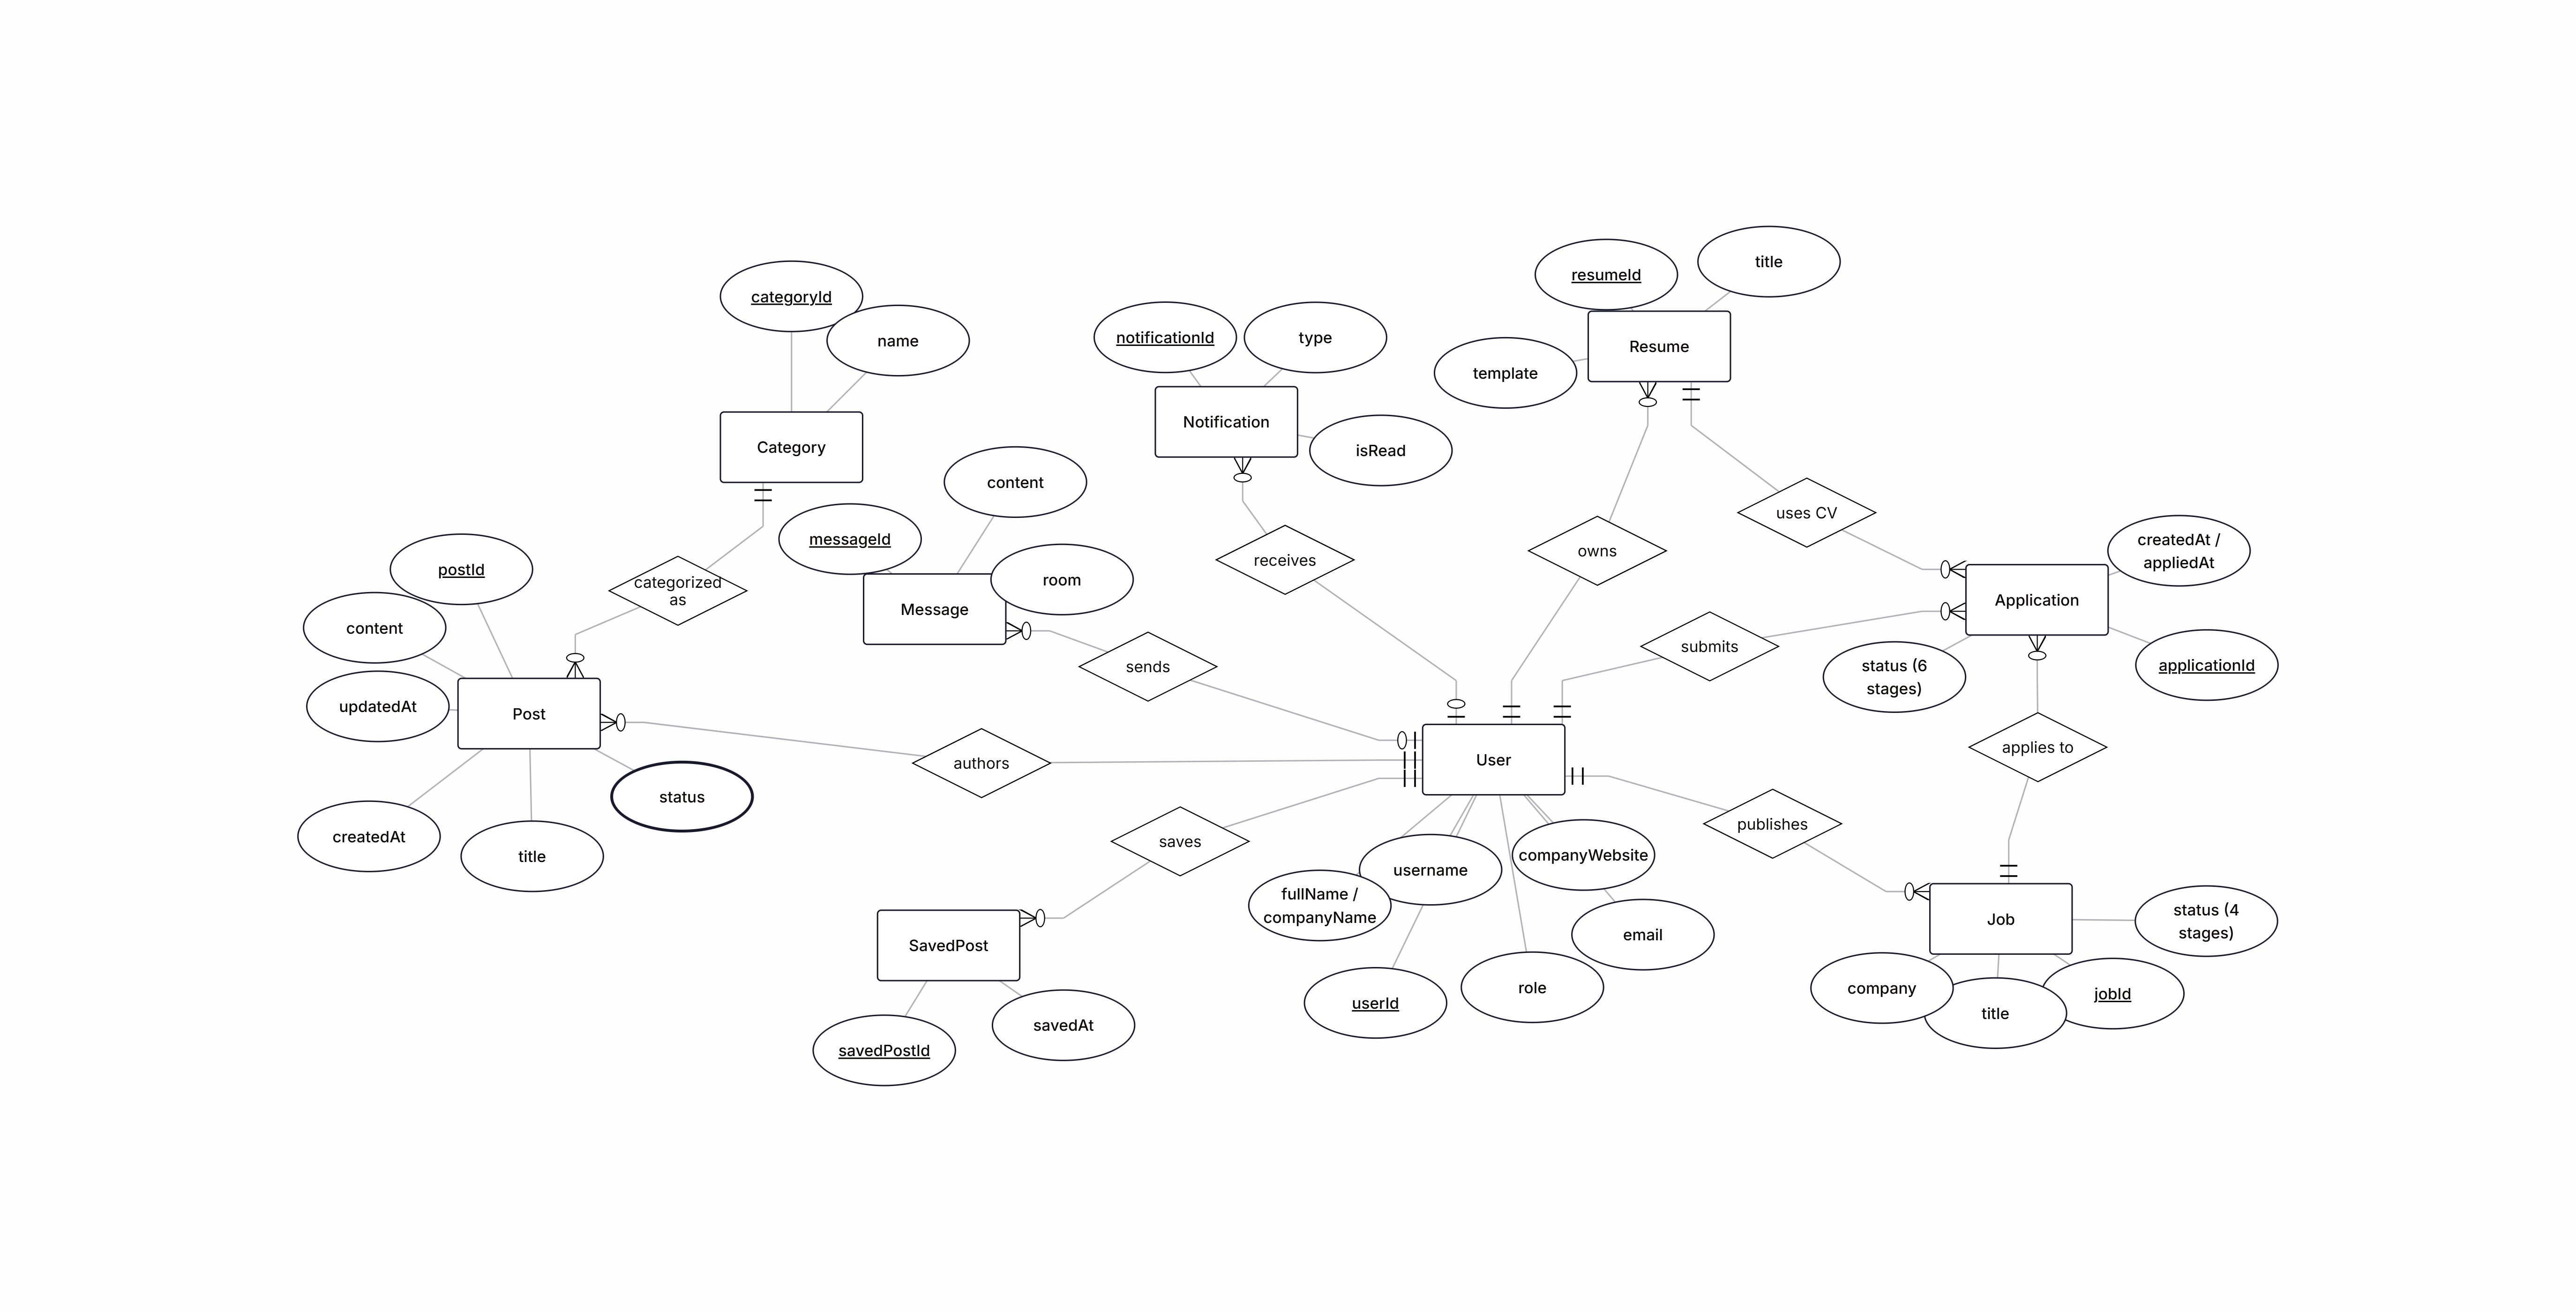
\includegraphics[
        trim=634bp 481bp 634bp 481bp,
        clip,
        angle=90,
        height=0.85\textheight,
        keepaspectratio
    ]{img/ERD.png}
    \caption{Lược đồ thực thể - mối quan hệ (ERD)}
    \label{fig:ERD}
\end{figure}

Dựa trên lược đồ ERD (Hình~\ref{fig:ERD}), mô hình dữ liệu của hệ thống được tổ chức xoay quanh thực thể trung tâm \texttt{User} cùng các mối quan hệ nghiệp vụ chính:

\begin{itemize}
    \item \textbf{Người dùng (\texttt{User}):}
    Là thực thể trung tâm, lưu thông tin tài khoản, hồ sơ cá nhân, vai trò và trạng thái hoạt động. Trường \texttt{role} được sử dụng để phân biệt ứng viên, doanh nghiệp và quản trị viên.

    \item \textbf{CV (\texttt{Resume}):}
    Lưu thông tin CV thuộc sở hữu của ứng viên. Mỗi CV tham chiếu đến một người dùng thông qua trường \texttt{userId}. Các nhóm thông tin như thông tin cá nhân, kinh nghiệm, học vấn, kỹ năng, ngoại ngữ, chứng chỉ, dự án, giải thưởng và sở thích được nhúng trực tiếp bên trong tài liệu CV vì chúng gắn liền với CV và thường xuyên được truy xuất đồng thời.

    \item \textbf{Tin tuyển dụng (\texttt{Job}):}
    Lưu thông tin vị trí tuyển dụng, doanh nghiệp, địa điểm, hình thức làm việc, mức lương, yêu cầu, quyền lợi và trạng thái của tin. Mỗi tin tuyển dụng tham chiếu đến tài khoản doanh nghiệp tạo tin thông qua trường \texttt{companyId}.

    \item \textbf{Hồ sơ ứng tuyển (\texttt{Application}):}
    Đại diện cho một lần ứng viên nộp CV vào một tin tuyển dụng. Mỗi tài liệu lưu trữ liên kết với ứng viên, tin tuyển dụng, CV tham chiếu, kèm theo bản chụp thông tin công việc (\texttt{jobSnapshot}) và bản chụp toàn vẹn CV (\texttt{resumeSnapshot}) tại thời điểm nộp để bảo đảm tính toàn vẹn và bất biến của hồ sơ ứng tuyển.

    \item \textbf{Công việc đã lưu (\texttt{SavedJob}):}
    Lưu danh sách các tin tuyển dụng được ứng viên đánh dấu lưu lại để theo dõi hoặc ứng tuyển sau, liên kết với ứng viên (\texttt{userId}) và bài đăng (\texttt{jobId}).

    \item \textbf{Tin nhắn (\texttt{Message}):}
    Lưu nội dung tin nhắn, người gửi, thời điểm gửi và phòng trò chuyện. Các tin nhắn được nhóm theo \texttt{room}, cho phép hệ thống truy xuất lịch sử trao đổi giữa ứng viên và nhà tuyển dụng.

    \item \textbf{Thông báo (\texttt{Notification}):}
    Thông báo được gửi đến người dùng khi xảy ra các sự kiện như có hồ sơ ứng tuyển mới, trạng thái ứng tuyển thay đổi hoặc tin tuyển dụng sắp hết hạn.

    \item \textbf{Lịch sử sử dụng AI (\texttt{AiUsage}):}
    Lưu lịch sử sử dụng các chức năng AI của từng người dùng, phục vụ việc kiểm tra hạn mức hằng ngày, thống kê và theo dõi trạng thái xử lý.

\end{itemize}


\subsection{Lược đồ quan hệ}


\begin{figure}[H]
    \centering
    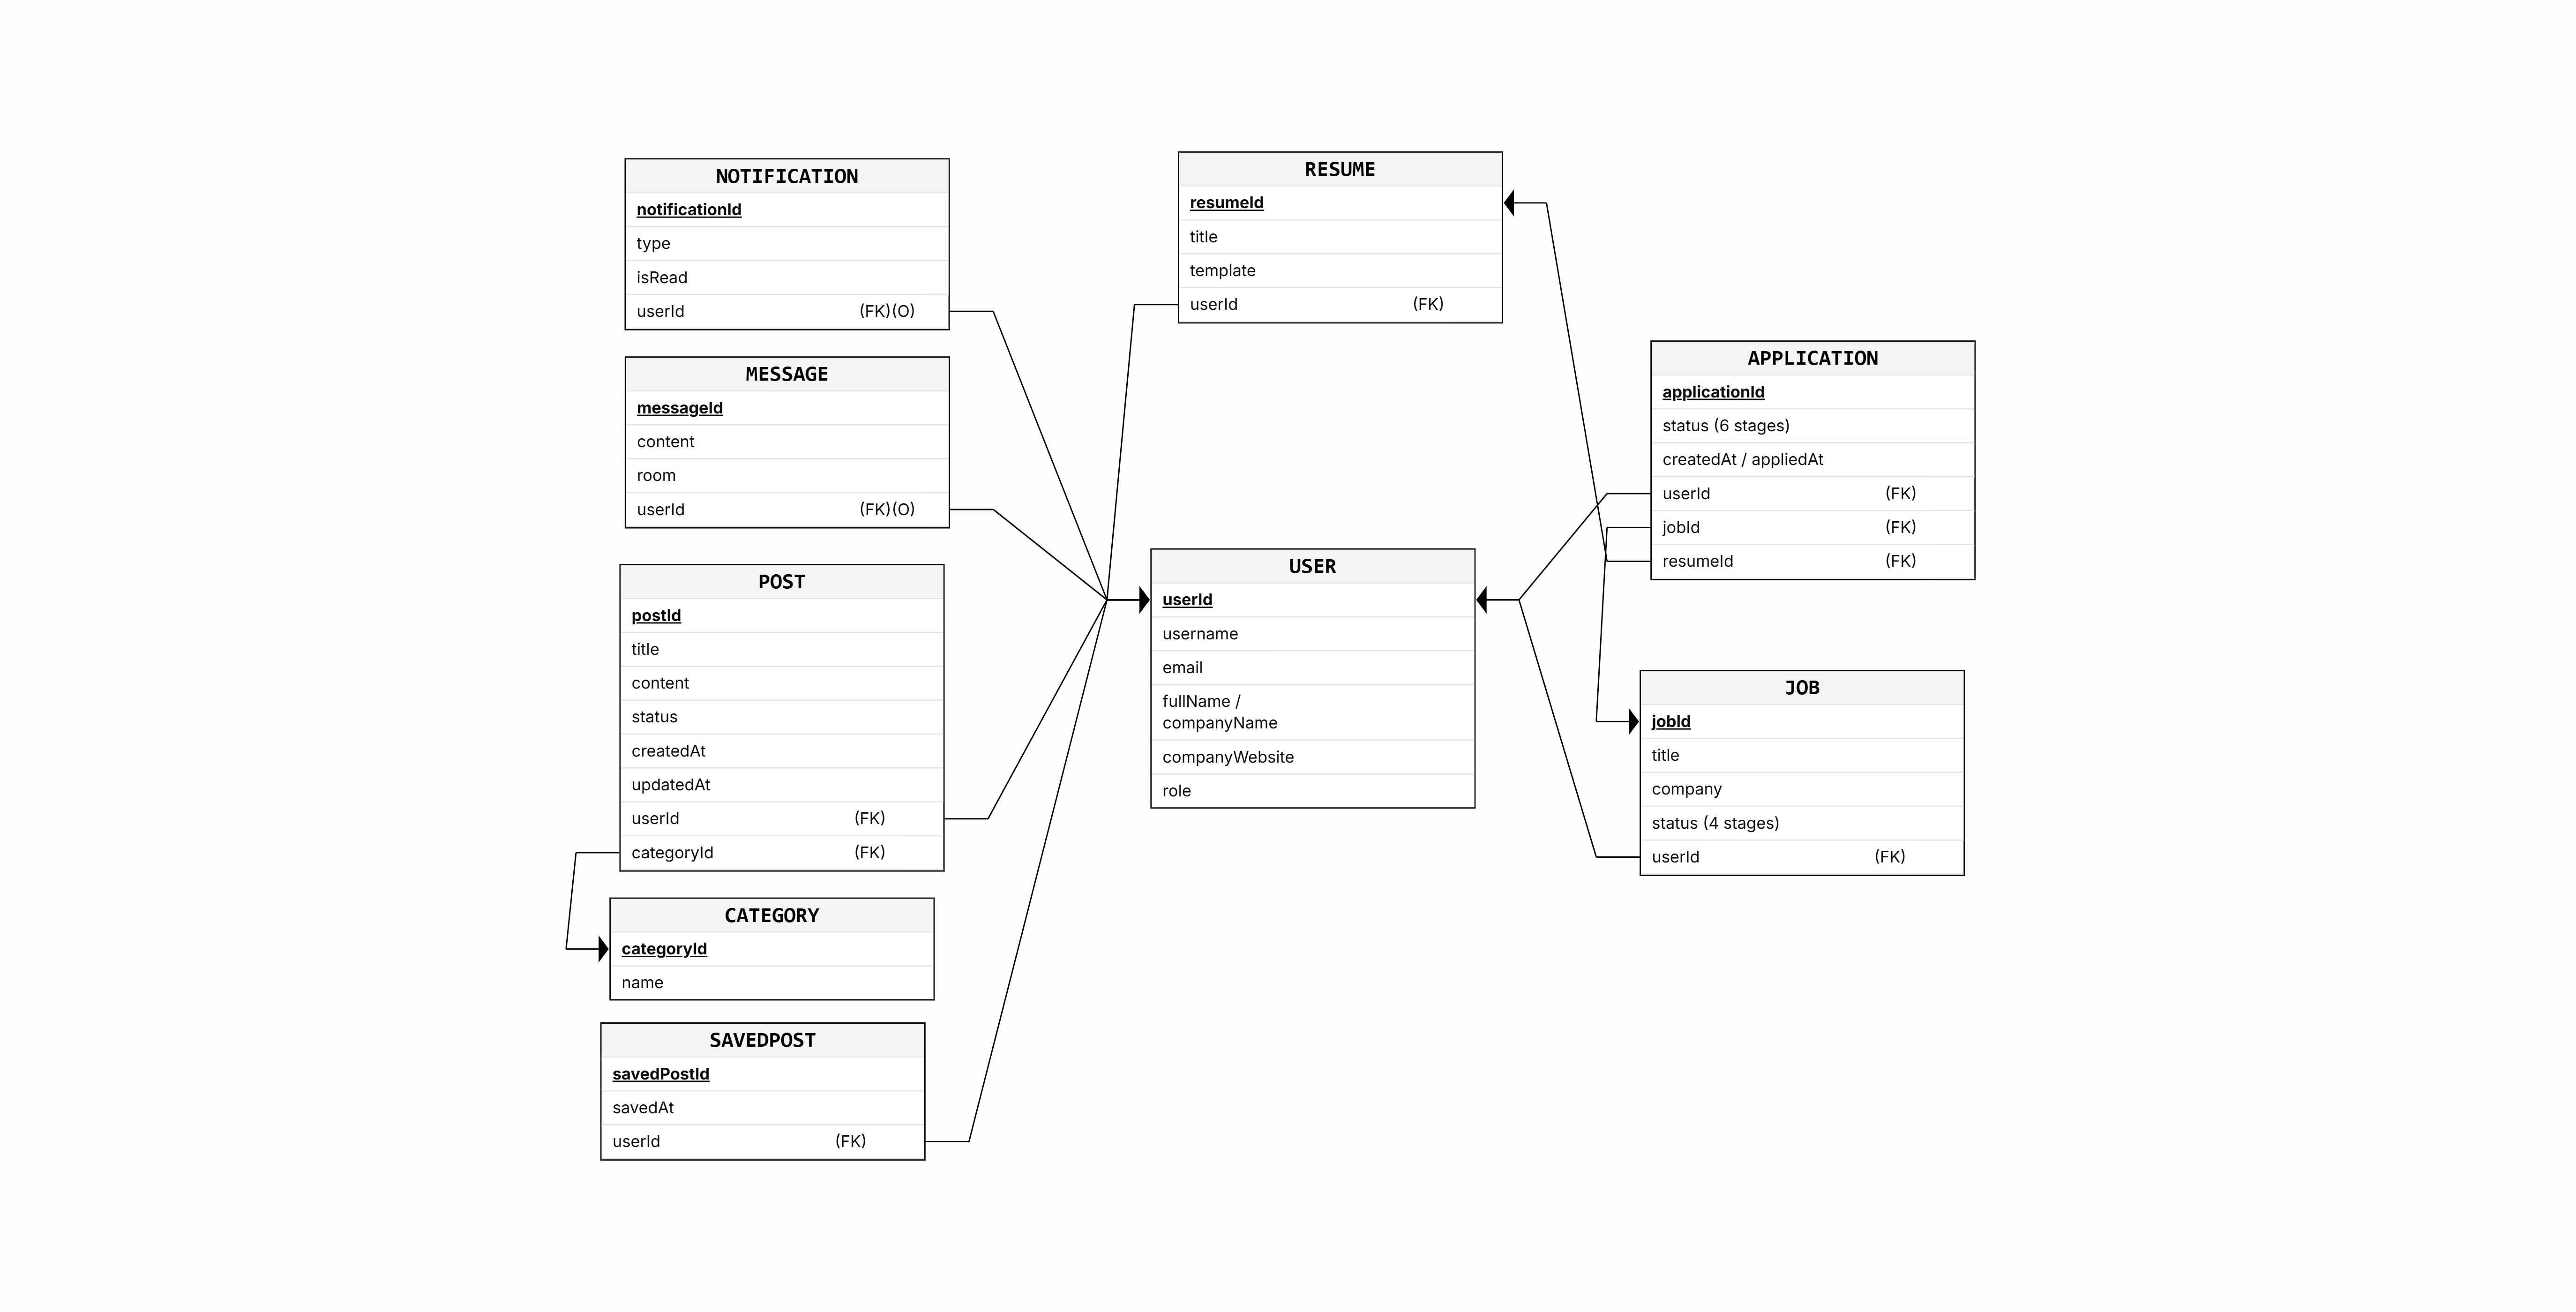
\includegraphics[
        trim=1200bp 320bp 1280bp 320bp,
        clip,
        width=\linewidth,
        keepaspectratio
    ]{img/relationalSchema.png}
    \caption{Lược đồ quan hệ}
    \label{fig:relationalSchema}
\end{figure}

Lược đồ quan hệ (Hình~\ref{fig:relationalSchema}) được chuyển dịch từ mô hình ERD nhằm mục đích tham khảo ở mức logic, giúp trực quan hóa mối quan hệ giữa các đối tượng trong hệ thống. Do RabbitCV sử dụng cơ sở dữ liệu NoSQL (MongoDB), hệ thống trên thực tế không sử dụng cấu trúc bảng hay các ràng buộc khóa chính, khóa ngoại vật lý như hệ CSDL quan hệ truyền thống, mà các liên kết dữ liệu được quản lý linh hoạt ở tầng ứng dụng thông qua mã định danh \texttt{\_id} (ObjectId) và cấu trúc tài liệu nhúng.

Về mặt logic nghiệp vụ, các thực thể và mối liên kết tham khảo được tổ chức theo các nhóm chức năng chính:

\begin{enumerate}
    \item \textbf{Quản lý tài khoản và hồ sơ người dùng}
    \begin{itemize}
        \item \textbf{User:} Lưu thông tin tài khoản, thông tin cá nhân, vai trò và trạng thái hoạt động của người dùng. Collection này đại diện chung cho ứng viên, doanh nghiệp và quản trị viên.

        \item \textbf{Resume:} Lưu CV của ứng viên và liên kết với người sở hữu thông qua trường \texttt{userId}. Các nhóm thông tin như thông tin cá nhân, kinh nghiệm, học vấn, kỹ năng, ngoại ngữ, chứng chỉ, dự án, giải thưởng và sở thích được nhúng trực tiếp trong tài liệu CV.
    \end{itemize}

    \item \textbf{Quản lý tuyển dụng và ứng tuyển}
    \begin{itemize}
        \item \textbf{Job:} Lưu thông tin tin tuyển dụng. Mỗi tin tuyển dụng liên kết với tài khoản doanh nghiệp thông qua trường \texttt{companyId}.

        \item \textbf{Application:} Lưu thông tin hồ sơ ứng tuyển của ứng viên vào một vị trí việc làm cụ thể, bao gồm liên kết tin tuyển dụng, ứng viên, trạng thái xét duyệt, bản chụp thông tin việc làm (\texttt{jobSnapshot}) và bản chụp CV (\texttt{resumeSnapshot}).

        \item \textbf{SavedJob:} Lưu thông tin công việc mà ứng viên đã lưu lại để tham khảo hoặc nộp hồ sơ sau, liên kết giữa ứng viên và bài đăng tuyển dụng.
    \end{itemize}

    \item \textbf{Quản lý trò chuyện và thông báo}
    \begin{itemize}
        \item \textbf{Message:} Lưu nội dung tin nhắn, người gửi, thời điểm gửi và phòng trò chuyện. Các tin nhắn thuộc cùng một cuộc trò chuyện được nhóm thông qua \texttt{room}.

        \item \textbf{Notification:} Lưu các thông báo phát sinh từ quá trình tuyển dụng như có hồ sơ ứng tuyển mới, thay đổi trạng thái hồ sơ hoặc tin nhắn mới.
    \end{itemize}

    \item \textbf{Quản lý hoạt động trí tuệ nhân tạo}
    \begin{itemize}
        \item \textbf{AiUsage:} Lưu thông tin về các lượt sử dụng các chức năng AI, bao gồm người sử dụng, chức năng được gọi, trạng thái, số token, thời gian phản hồi và mã lỗi. Dữ liệu này hỗ trợ theo dõi hoạt động và áp dụng hạn mức.
    \end{itemize}

\end{enumerate}

% \begin{table}[H]
%     \centering
%     \small
%     \begin{tabularx}{\textwidth}{|p{0.13\textwidth}|p{0.21\textwidth}|Y|} \hline
%         \textbf{Mã} & \textbf{Nhóm} & \textbf{Tiêu chí kiểm chứng} \\ \hline
%         NFR-SEC-01 & Xác thực & Mọi API riêng tư và toàn bộ route AI yêu cầu JWT hợp lệ; thao tác đặc quyền phải kiểm tra vai trò ở backend. API chung, đăng nhập, đăng ký và AI có giới hạn tần suất riêng. \\ \hline
%         NFR-SEC-02 & Quyền dữ liệu & Resume chỉ được trả cho chủ sở hữu, admin hoặc doanh nghiệp có quan hệ nghiệp vụ phù hợp. \\ \hline
%         NFR-PDF-01 & Tài liệu & CV web dùng kích thước A4; PDF upload phải có header hợp lệ và kích thước giải mã không quá 5 MB. \\ \hline
%         NFR-AI-01 & Kiểm soát AI & Rate limit 30 request/15 phút; quota ngày và timeout có thể cấu hình, mặc định lần lượt là 100 request và 20 giây. \\ \hline
%         NFR-AI-02 & Hợp đồng dữ liệu & Request AI loại thông tin liên hệ trực tiếp; response phải khớp JSON Schema và được làm sạch trước khi trả frontend. \\ \hline
%         NFR-DATA-01 & Toàn vẹn & Unique index ngăn ứng tuyển trùng; snapshot giữ lịch sử; thao tác ẩn/đọc chat không xóa dữ liệu của bên còn lại. \\ \hline
%         NFR-TEST-01 & Khả năng tái lập & Quy trình \texttt{npm run check} phải chạy ESLint, 43 test hiện có và Vite build; kết quả phải gắn với ngày, phiên bản runtime và trạng thái working tree. \\ \hline
%         NFR-UX-01 & Khả dụng & Kết quả AI chỉ là gợi ý, có trạng thái chờ/lỗi và không tự ghi đè nội dung khi người dùng chưa xác nhận. \\ \hline
%     \end{tabularx}
%     \caption{Yêu cầu phi chức năng có tiêu chí kiểm chứng}
%     \label{tab:nonfunctional-requirements}
% \end{table}

% \section{Ma trận phân quyền}

% \begin{table}[H]
%     \centering
%     \scriptsize
%     \begin{tabularx}{\textwidth}{|Y|c|c|c|c|} \hline
%         \textbf{Chức năng} & \textbf{Khách} & \textbf{Ứng viên} & \textbf{Doanh nghiệp} & \textbf{Admin} \\ \hline
%         Xem danh sách/chi tiết việc công khai & Có & Có & Có & Có \\ \hline
%         Tạo, sửa và dùng AI cho CV cá nhân & Không & Có & Không & Giới hạn \\ \hline
%         Lưu việc và nộp hồ sơ & Không & Có & Không & Không \\ \hline
%         Tạo và quản lý tin tuyển dụng & Không & Không & Tin sở hữu & Đặc quyền \\ \hline
%         Xem CV ứng viên & Không & CV sở hữu & Hồ sơ liên quan & Đặc quyền \\ \hline
%         Cập nhật trạng thái Application & Không & Không & Hồ sơ thuộc tin sở hữu & Đặc quyền \\ \hline
%         Nhắn tin và đọc thông báo & Không & Có & Có & Theo phạm vi \\ \hline
%         Quản lý người dùng/doanh nghiệp & Không & Không & Không & Có \\ \hline
%     \end{tabularx}
%     \caption{Ma trận quyền theo tác nhân}
%     \label{tab:role-matrix}
% \end{table}

% Ma trận trên mô tả chính sách mong muốn ở mức nghiệp vụ. Frontend có thể ẩn hoặc chuyển hướng giao diện, nhưng quyết định cuối cùng phải do middleware và truy vấn có điều kiện ở backend thực hiện. Qua đối chiếu mã nguồn hiện tại, nhóm API AI mới yêu cầu JWT chung và chưa kiểm tra riêng vai trò ứng viên; một số endpoint lưu việc và chat cũng mới dừng ở mức xác thực. Đây là khoảng cách giữa chính sách và hiện thực cần được kiểm thử, bổ sung trước khi triển khai thực tế.

% \section{Kiến trúc tổng thể}

% RabbitCV là ứng dụng client--server, không phải microservice. Frontend và backend có thể đóng gói/chạy riêng nhưng backend hiện tập trung phần lớn REST route trong \texttt{server/server.js}. Route AI, schema, service gọi nhà cung cấp, sanitizer và hàm xử lý hạn tin được tách thành các module riêng. Ở frontend, Context quản lý phiên và socket; TanStack Query quản lý một phần dữ liệu máy chủ; React Hook Form và Zod quản lý biểu mẫu xác thực.

% \begin{figure}[H]
%     \centering
%     \resizebox{0.98\textwidth}{!}{%
%     \begin{tikzpicture}[
%         box/.style={draw, rounded corners, align=center, minimum height=1.05cm, minimum width=2.7cm, fill=blue!5},
%         ext/.style={draw, rounded corners, align=center, minimum height=1.05cm, minimum width=2.5cm, fill=orange!10},
%         arr/.style={-Latex, line width=0.8pt}
%     ]
%         \node[box] (browser) {Trình duyệt\\React + Router};
%         \node[box, right=1.1cm of browser] (contexts) {Context + Query/Form\\Tailwind + Tiptap};
%         \node[box, right=1.1cm of contexts] (api) {Express REST API\\JWT + rate limit};
%         \node[box, right=1.1cm of api] (models) {Service/Utility\\Mongoose models};
%         \node[box, right=1.1cm of models] (db) {MongoDB};
%         \node[ext, below=1.1cm of api] (socket) {Socket.IO\\room người dùng};
%         \node[ext, below=1.1cm of models] (cron) {Vercel Cron\\HTTP GET có token};
%         \node[ext, above=1.1cm of models] (groq) {Groq API\\LLM + JSON Schema};
%         \node[ext, above=1.1cm of contexts] (pdf) {PDF.js\\trình kết xuất};

%         \draw[arr,<->] (browser) -- node[above]{HTTP} (contexts);
%         \draw[arr,<->] (contexts) -- node[above]{JSON} (api);
%         \draw[arr,<->] (api) -- (models);
%         \draw[arr,<->] (models) -- (db);
%         \draw[arr,<->] (contexts) -- (socket);
%         \draw[arr,<->] (socket) -- (api);
%         \draw[arr] (cron) -- (api);
%         \draw[arr,<->] (api) -- (groq);
%         \draw[arr] (contexts) -- (pdf);
%     \end{tikzpicture}}
%     \caption{Kiến trúc triển khai của RabbitCV}
%     \label{fig:system-architecture}
% \end{figure}

% \section{Thiết kế mô-đun}

% \begin{table}[H]
%     \centering
%     \small
%     \begin{tabularx}{\textwidth}{|p{0.20\textwidth}|p{0.28\textwidth}|Y|} \hline
%         \textbf{Mô-đun} & \textbf{Thành phần chính} & \textbf{Trách nhiệm} \\ \hline
%         Phiên và vai trò & AuthContext, RoleAccessGuard, authMiddleware. & Đăng ký, đăng nhập, khôi phục phiên, đăng xuất, chuyển hướng và kiểm tra quyền. \\ \hline
%         Dữ liệu giao diện & QueryClient, SavedJobsContext, useNotifications, form schema. & Cache dữ liệu máy chủ, polling, cập nhật lạc quan, khôi phục khi lỗi và kiểm tra biểu mẫu. \\ \hline
%         CV & ResumeForm, ResumePreview, Resume model. & Dữ liệu CV, template, preview A4, in PDF, CV upload và quyền sở hữu. \\ \hline
%         AI & aiRoutes, aiService, aiSchemas, sanitizer, AiUsage. & Chuẩn hóa input, quota, gọi model, kiểm tra schema, lọc output và thống kê. \\ \hline
%         Việc làm & Jobs, JobDetail, Job/Application models. & Tìm kiếm, trạng thái tin, lưu việc, ứng tuyển, snapshot và xử lý hồ sơ. \\ \hline
%         Giao tiếp & Message, SocketContext, NotificationBell. & Lưu message, phát event, trạng thái đọc/ẩn room và thông báo. \\ \hline
%         Doanh nghiệp & CompanyDashboard và API Job/Application. & Hồ sơ công ty, tin tuyển dụng, danh sách ứng viên và cập nhật trạng thái. \\ \hline
%         Quản trị & AdminLayout và nhóm API admin. & Thống kê, người dùng, doanh nghiệp và tin tuyển dụng. \\ \hline
%     \end{tabularx}
%     \caption{Phân rã mô-đun theo thành phần triển khai}
%     \label{tab:module-design}
% \end{table}

% \section{Thiết kế dữ liệu}

% MongoDB dùng reference ObjectId giữa các tài liệu thay vì lược đồ quan hệ vật lý. Hình \ref{fig:data-model} thể hiện quan hệ nghiệp vụ chính; các mũi tên không có nghĩa database tự áp dụng khóa ngoại.

% \begin{figure}[H]
%     \centering
%     \resizebox{0.96\textwidth}{!}{%
%     \begin{tikzpicture}[
%         entity/.style={draw, rounded corners, align=left, text width=3.15cm, inner sep=4pt, minimum height=1.05cm, fill=green!6, font=\small},
%         rel/.style={-Latex, line width=0.75pt}
%     ]
%         \node[entity] (user) at (5.8,6.0) {\textbf{User}\\role, profile, savedJobs};
%         \node[entity] (msg) at (-0.2,3.0) {\textbf{Message}\\sender, room, content};
%         \node[entity] (resume) at (3.8,3.0) {\textbf{Resume}\\userId, sections, pdfData};
%         \node[entity] (job) at (7.8,3.0) {\textbf{Job}\\companyId, status, expiryDate};
%         \node[entity] (usage) at (11.8,3.0) {\textbf{AiUsage}\\userId, feature, model\\latency, token, status};
%         \node[entity] (read) at (0.4,0) {\textbf{ChatReadState /}\\\textbf{HiddenChat}\\userId, room, lastReadAt};
%         \node[entity] (app) at (5.8,0) {\textbf{Application}\\jobId, candidateId, resumeId\\jobSnapshot, status};
%         \node[entity] (noti) at (11.0,0) {\textbf{Notification}\\recipient, type, isRead};

%         \draw[rel] (user) -- (msg);
%         \draw[rel] (user) -- (resume);
%         \draw[rel] (user) -- (job);
%         \draw[rel] (user) -- (usage);
%         \draw[rel] (user) -- (app);
%         \draw[rel] (resume) -- (app);
%         \draw[rel] (job) -- (app);
%         \draw[rel] (msg) -- (read);
%         \draw[rel] (app) -- (noti);
%     \end{tikzpicture}}
%     \caption{Mô hình quan hệ giữa các collection chính}
%     \label{fig:data-model}
% \end{figure}

% \subsection{User và Resume}

% User lưu username, email, mật khẩu băm, vai trò, trạng thái tài khoản, hồ sơ ứng viên hoặc công ty và danh sách Job đã lưu. Resume tham chiếu \texttt{userId}, chứa dữ liệu CV có cấu trúc, mẫu và metadata. \texttt{isVirtual} phân biệt PDF tạm được tạo khi ứng tuyển với CV cấu trúc do người dùng quản lý; \texttt{pdfData} chỉ có ý nghĩa với CV PDF và bị loại khỏi truy vấn danh sách.

% \subsection{Job và Application}

% Job liên kết doanh nghiệp qua \texttt{companyId}, chứa nội dung, trạng thái và ngày hết hạn. Application liên kết Job, ứng viên và Resume. Unique index trên \texttt{jobId}--\texttt{candidateId} ngăn hồ sơ trùng. \texttt{jobSnapshot} lưu tiêu đề, công ty, địa điểm, loại và lương tại thời điểm nộp để lịch sử không mất ngữ cảnh khi Job bị xóa.

% \subsection{Message, Notification và trạng thái đọc}

% Message lưu sender, room và nội dung. ChatReadState lưu \texttt{lastReadAt} theo cặp user--room; HiddenChat ghi việc một phía ẩn room. Notification lưu recipient, nội dung, liên kết và \texttt{isRead}. Thiết kế này tách trạng thái cá nhân khỏi dữ liệu trao đổi chung.

% \subsection{AiUsage}

% AiUsage lưu user, feature, model, hash đầu vào, trạng thái, token, độ trễ và mã lỗi. Dữ liệu này hỗ trợ quota và quan sát kỹ thuật mà không cần lưu nguyên prompt hoặc toàn bộ CV. Hash không được dùng như cơ chế ẩn danh tuyệt đối; hệ thống vẫn cần hạn chế quyền truy cập collection thống kê.

% \section{Các quy trình nghiệp vụ chính}

% \subsection{Ứng tuyển bằng CV}

% \begin{figure}[H]
%     \centering
%     \resizebox{0.96\textwidth}{!}{%
%     \begin{tikzpicture}[
%         flowstep/.style={draw, rounded corners, align=center, minimum width=2.65cm, minimum height=1.05cm, fill=purple!7},
%         arr/.style={-Latex, line width=0.8pt}
%     ]
%         \node[flowstep] (select) {Ứng viên chọn\\Job và CV};
%         \node[flowstep, right=0.65cm of select] (auth) {Xác thực và\\quyền sở hữu CV};
%         \node[flowstep, right=0.65cm of auth] (check) {Kiểm tra Job\\hạn và trạng thái};
%         \node[flowstep, right=0.65cm of check] (unique) {Kiểm tra unique\\Application};
%         \node[flowstep, right=0.65cm of unique] (save) {Lưu Application\\và jobSnapshot};
%         \node[flowstep, right=0.65cm of save] (notify) {Tạo thông báo\\trả kết quả};
%         \draw[arr] (select) -- (auth);
%         \draw[arr] (auth) -- (check);
%         \draw[arr] (check) -- (unique);
%         \draw[arr] (unique) -- (save);
%         \draw[arr] (save) -- (notify);
%     \end{tikzpicture}}
%     \caption{Luồng kiểm soát khi ứng tuyển bằng CV}
%     \label{fig:application-flow}
% \end{figure}

% Với PDF upload, backend kiểm tra data URL, MIME, đuôi, header và dung lượng giải mã; sau đó tạo Resume ảo và tiếp tục cùng luồng Application. Nếu bất kỳ kiểm tra nào thất bại, không tạo Resume hoặc Application mới.

% \subsection{Yêu cầu AI}

% \begin{figure}[H]
%     \centering
%     \resizebox{0.98\textwidth}{!}{%
%     \begin{tikzpicture}[
%         flowstep/.style={draw, rounded corners, align=center, minimum width=2.45cm, minimum height=1.05cm, fill=orange!9},
%         arr/.style={-Latex, line width=0.8pt}
%     ]
%         \node[flowstep] (ui) {UI gửi feature\\và context};
%         \node[flowstep, right=0.5cm of ui] (gate) {JWT, rate limit\\quota ngày};
%         \node[flowstep, right=0.5cm of gate] (clean) {Sanitize và\\rút gọn dữ liệu};
%         \node[flowstep, right=0.5cm of clean] (schema) {Chọn instruction\\và JSON Schema};
%         \node[flowstep, right=0.5cm of schema] (provider) {Groq LLM\\structured output};
%         \node[flowstep, right=0.5cm of provider] (validate) {Parse, kiểm tra\\nghiệp vụ và lọc};
%         \node[flowstep, right=0.5cm of validate] (result) {Gợi ý + meta\\người dùng áp dụng};
%         \draw[arr] (ui) -- (gate);
%         \draw[arr] (gate) -- (clean);
%         \draw[arr] (clean) -- (schema);
%         \draw[arr] (schema) -- (provider);
%         \draw[arr] (provider) -- (validate);
%         \draw[arr] (validate) -- (result);
%     \end{tikzpicture}}
%     \caption{Đường đi của dữ liệu trong một yêu cầu AI}
%     \label{fig:ai-request-flow}
% \end{figure}

% Service tạo bản ghi AiUsage trước khi gọi nhà cung cấp và cập nhật trạng thái sau khi hoàn tất hoặc thất bại. Nhà cung cấp được yêu cầu áp dụng JSON Schema nghiêm ngặt; backend tiếp tục kiểm tra điều kiện ngữ nghĩa ở luồng tiểu sử và làm sạch/giới hạn đầu ra ở luồng điền CV, phỏng vấn. Frontend nhận lưu ý cùng kết quả ở các chức năng review, chấm CV và phỏng vấn. Không có bước tự động lưu kết quả AI vào Resume.

% \subsection{Chat và trạng thái đọc}

% Người gửi gọi REST API; server lấy định danh và tên người gửi từ tài khoản đã xác thực, kiểm tra tin có nội dung hoặc ảnh, lưu Message rồi phát \texttt{newMessage} đến phòng của người nhận. Văn bản chat được React hiển thị như chuỗi, còn ảnh được nén ở client trước khi chuyển thành data URL. Khi mở phòng, client cập nhật \texttt{lastReadAt}. Việc ẩn phòng tạo hoặc cập nhật HiddenChat theo user; Message của phía còn lại không bị xóa. Notification không dùng chung kênh này mà được tải qua API, do đó có thể có độ trễ tối đa theo chu kỳ polling.

% \section{Bảo mật và ranh giới tin cậy}

% Thiết kế xác định ba ranh giới tin cậy chính:

% \begin{itemize}
%     \item \textbf{Giữa trình duyệt và backend:} mọi dữ liệu từ client đều không đáng tin, kể cả vai trò hoặc mã người dùng.
%     \item \textbf{Giữa backend và dịch vụ AI:} chỉ dữ liệu đã được làm sạch, giới hạn và thật sự cần thiết mới được gửi ra ngoài.
%     \item \textbf{Tại dữ liệu CV:} đường dẫn xem CV phải kiểm tra quan hệ sở hữu hoặc quan hệ tuyển dụng, không chỉ kiểm tra người gọi đã đăng nhập.
% \end{itemize}

% Các biện pháp kiểm soát hiện có được chia thành các nhóm sau:

% \begin{itemize}
%     \item \textbf{Xác thực và bảo vệ HTTP:} bcryptjs, JWT trong cookie HTTP-only, Helmet, CSP, CORS theo danh sách nguồn và giới hạn tốc độ.
%     \item \textbf{Kiểm tra dữ liệu và quyền truy cập:} kiểm tra ObjectId, danh sách trường người dùng theo ngữ cảnh, bộ làm sạch rich text/PDF/AI, chỉ mục duy nhất và truy vấn kèm điều kiện sở hữu.
%     \item \textbf{Giới hạn thông tin vận hành:} health check công khai chỉ trả trạng thái tối giản; thông tin môi trường và cơ sở dữ liệu chi tiết yêu cầu quyền quản trị.
%     \item \textbf{Phạm vi bảo vệ:} các biện pháp trên giúp giảm rủi ro nhưng không thay thế kiểm thử xâm nhập, phân tích CSRF, quản lý bí mật production hoặc rà soát đầy đủ ma trận quyền.
% \end{itemize}

% \noindent\textbf{Hạn chế của thiết kế hiện tại.}
% Backend còn tập trung nhiều route trong một file; PDF và ảnh chat dạng data URL làm tài liệu MongoDB lớn; notification dùng polling; Socket.IO trên môi trường serverless chưa phải kiến trúc phù hợp cho tải lớn. Tác vụ theo lịch chưa có kiểm thử về gọi đồng thời, retry và quan sát lỗi. Mã nguồn vẫn có khóa JWT dự phòng và cơ chế tạo tài khoản quản trị phục vụ trình diễn; chúng phải bị vô hiệu hóa hoặc bắt buộc cấu hình ở production. Đặc biệt, API gửi/ẩn chat chưa kiểm tra đầy đủ người gọi có thuộc phòng và API AI chưa chặn theo vai trò ứng viên. Phần AI còn phụ thuộc nhà cung cấp và model cấu hình, trong khi chất lượng ngữ nghĩa chưa có bộ dữ liệu chấm độc lập. Các hạn chế này được chuyển thành mục kiểm thử hoặc hướng phát triển thay vì được mô tả như chức năng đã hoàn tất.
